\documentclass[twoside]{book}

% Packages required by doxygen
\usepackage{fixltx2e}
\usepackage{calc}
\usepackage{doxygen}
\usepackage[export]{adjustbox} % also loads graphicx
\usepackage{graphicx}
\usepackage[utf8]{inputenc}
\usepackage{makeidx}
\usepackage{multicol}
\usepackage{multirow}
\PassOptionsToPackage{warn}{textcomp}
\usepackage{textcomp}
\usepackage[nointegrals]{wasysym}
\usepackage[table]{xcolor}

% Font selection
\usepackage[T1]{fontenc}
\usepackage[scaled=.90]{helvet}
\usepackage{courier}
\usepackage{amssymb}
\usepackage{sectsty}
\renewcommand{\familydefault}{\sfdefault}
\allsectionsfont{%
  \fontseries{bc}\selectfont%
  \color{darkgray}%
}
\renewcommand{\DoxyLabelFont}{%
  \fontseries{bc}\selectfont%
  \color{darkgray}%
}
\newcommand{\+}{\discretionary{\mbox{\scriptsize$\hookleftarrow$}}{}{}}

% Page & text layout
\usepackage{geometry}
\geometry{%
  a4paper,%
  top=2.5cm,%
  bottom=2.5cm,%
  left=2.5cm,%
  right=2.5cm%
}
\tolerance=750
\hfuzz=15pt
\hbadness=750
\setlength{\emergencystretch}{15pt}
\setlength{\parindent}{0cm}
\setlength{\parskip}{3ex plus 2ex minus 2ex}
\makeatletter
\renewcommand{\paragraph}{%
  \@startsection{paragraph}{4}{0ex}{-1.0ex}{1.0ex}{%
    \normalfont\normalsize\bfseries\SS@parafont%
  }%
}
\renewcommand{\subparagraph}{%
  \@startsection{subparagraph}{5}{0ex}{-1.0ex}{1.0ex}{%
    \normalfont\normalsize\bfseries\SS@subparafont%
  }%
}
\makeatother

% Headers & footers
\usepackage{fancyhdr}
\pagestyle{fancyplain}
\fancyhead[LE]{\fancyplain{}{\bfseries\thepage}}
\fancyhead[CE]{\fancyplain{}{}}
\fancyhead[RE]{\fancyplain{}{\bfseries\leftmark}}
\fancyhead[LO]{\fancyplain{}{\bfseries\rightmark}}
\fancyhead[CO]{\fancyplain{}{}}
\fancyhead[RO]{\fancyplain{}{\bfseries\thepage}}
\fancyfoot[LE]{\fancyplain{}{}}
\fancyfoot[CE]{\fancyplain{}{}}
\fancyfoot[RE]{\fancyplain{}{\bfseries\scriptsize Generated by Doxygen }}
\fancyfoot[LO]{\fancyplain{}{\bfseries\scriptsize Generated by Doxygen }}
\fancyfoot[CO]{\fancyplain{}{}}
\fancyfoot[RO]{\fancyplain{}{}}
\renewcommand{\footrulewidth}{0.4pt}
\renewcommand{\chaptermark}[1]{%
  \markboth{#1}{}%
}
\renewcommand{\sectionmark}[1]{%
  \markright{\thesection\ #1}%
}

% Indices & bibliography
\usepackage{natbib}
\usepackage[titles]{tocloft}
\setcounter{tocdepth}{3}
\setcounter{secnumdepth}{5}
\makeindex

% Hyperlinks (required, but should be loaded last)
\usepackage{ifpdf}
\ifpdf
  \usepackage[pdftex,pagebackref=true]{hyperref}
\else
  \usepackage[ps2pdf,pagebackref=true]{hyperref}
\fi
\hypersetup{%
  colorlinks=true,%
  linkcolor=blue,%
  citecolor=blue,%
  unicode%
}

% Custom commands
\newcommand{\clearemptydoublepage}{%
  \newpage{\pagestyle{empty}\cleardoublepage}%
}

\usepackage{caption}
\captionsetup{labelsep=space,justification=centering,font={bf},singlelinecheck=off,skip=4pt,position=top}

%===== C O N T E N T S =====

\begin{document}

% Titlepage & ToC
\hypersetup{pageanchor=false,
             bookmarksnumbered=true,
             pdfencoding=unicode
            }
\pagenumbering{roman}
\begin{titlepage}
\vspace*{7cm}
\begin{center}%
{\Large Modbus\+\_\+\+L\+P\+C1769 }\\
\vspace*{1cm}
{\large Generated by Doxygen 1.8.11}\\
\end{center}
\end{titlepage}
\clearemptydoublepage
\tableofcontents
\clearemptydoublepage
\pagenumbering{arabic}
\hypersetup{pageanchor=true}

%--- Begin generated contents ---
\chapter{File Index}
\section{File List}
Here is a list of all documented files with brief descriptions\+:\begin{DoxyCompactList}
\item\contentsline{section}{{\bfseries cr\+\_\+startup\+\_\+lpc175x\+\_\+6x.\+c} }{\pageref{cr__startup__lpc175x__6x_8c}}{}
\item\contentsline{section}{{\bfseries crp.\+c} }{\pageref{crp_8c}}{}
\item\contentsline{section}{\hyperlink{main_8c}{main.\+c} }{\pageref{main_8c}}{}
\item\contentsline{section}{\hyperlink{mb_8c}{mb.\+c} \\*This is main source file for G\+PI Module }{\pageref{mb_8c}}{}
\item\contentsline{section}{\hyperlink{mbcrc_8c}{mbcrc.\+c} }{\pageref{mbcrc_8c}}{}
\item\contentsline{section}{\hyperlink{mbfunccoils_8c}{mbfunccoils.\+c} }{\pageref{mbfunccoils_8c}}{}
\item\contentsline{section}{\hyperlink{mbfuncdisc_8c}{mbfuncdisc.\+c} }{\pageref{mbfuncdisc_8c}}{}
\item\contentsline{section}{\hyperlink{mbfuncholding_8c}{mbfuncholding.\+c} }{\pageref{mbfuncholding_8c}}{}
\item\contentsline{section}{\hyperlink{mbfuncinput_8c}{mbfuncinput.\+c} }{\pageref{mbfuncinput_8c}}{}
\item\contentsline{section}{\hyperlink{mbfuncother_8c}{mbfuncother.\+c} }{\pageref{mbfuncother_8c}}{}
\item\contentsline{section}{\hyperlink{mbrtu_8c}{mbrtu.\+c} }{\pageref{mbrtu_8c}}{}
\item\contentsline{section}{\hyperlink{mbutils_8c}{mbutils.\+c} }{\pageref{mbutils_8c}}{}
\item\contentsline{section}{\hyperlink{modbus_8c}{modbus.\+c} }{\pageref{modbus_8c}}{}
\item\contentsline{section}{\hyperlink{portevent_8c}{portevent.\+c} \\*This is main source file for G\+PI Module }{\pageref{portevent_8c}}{}
\item\contentsline{section}{\hyperlink{portserial_8c}{portserial.\+c} }{\pageref{portserial_8c}}{}
\item\contentsline{section}{\hyperlink{portserial_8h}{portserial.\+h} }{\pageref{portserial_8h}}{}
\item\contentsline{section}{\hyperlink{porttimer_8c}{porttimer.\+c} }{\pageref{porttimer_8c}}{}
\end{DoxyCompactList}

\chapter{File Documentation}
\hypertarget{main_8c}{}\section{main.\+c File Reference}
\label{main_8c}\index{main.\+c@{main.\+c}}
{\ttfamily \#include \char`\"{}mb.\+h\char`\"{}}\\*
{\ttfamily \#include \char`\"{}mbport.\+h\char`\"{}}\\*
Include dependency graph for main.\+c\+:\nopagebreak
\begin{figure}[H]
\begin{center}
\leavevmode
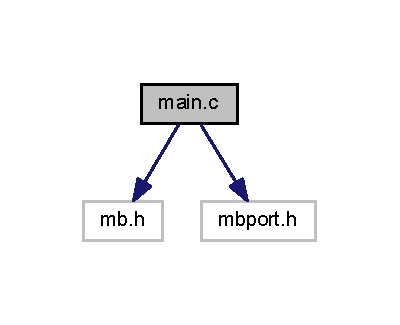
\includegraphics[width=192pt]{main_8c__incl}
\end{center}
\end{figure}
\subsection*{Macros}
\begin{DoxyCompactItemize}
\item 
\#define {\bfseries R\+E\+G\+\_\+\+I\+N\+P\+U\+T\+\_\+\+S\+T\+A\+RT}~1000\hypertarget{main_8c_a27bda6ca1eca28ed48c3fa6ada78ba5d}{}\label{main_8c_a27bda6ca1eca28ed48c3fa6ada78ba5d}

\item 
\#define {\bfseries R\+E\+G\+\_\+\+I\+N\+P\+U\+T\+\_\+\+N\+R\+E\+GS}~4\hypertarget{main_8c_ab2f42820482da2df43117b4dfe700eb2}{}\label{main_8c_ab2f42820482da2df43117b4dfe700eb2}

\item 
\#define {\bfseries S\+L\+A\+V\+E\+\_\+\+ID}~0x0A\hypertarget{main_8c_aed258e18fa2ea561f21f58d651a33cff}{}\label{main_8c_aed258e18fa2ea561f21f58d651a33cff}

\end{DoxyCompactItemize}
\subsection*{Functions}
\begin{DoxyCompactItemize}
\item 
int \hyperlink{main_8c_a840291bc02cba5474a4cb46a9b9566fe}{main} (void)
\item 
e\+M\+B\+Error\+Code \hyperlink{main_8c_a7816677520b1eb2ebecf15060a41bc81}{e\+M\+B\+Reg\+Input\+CB} (U\+C\+H\+AR $\ast$puc\+Reg\+Buffer, U\+S\+H\+O\+RT us\+Address, U\+S\+H\+O\+RT us\+N\+Regs)
\item 
e\+M\+B\+Error\+Code \hyperlink{main_8c_a10d37e1d80224bf3b1eeb9e246d7582e}{e\+M\+B\+Reg\+Holding\+CB} (U\+C\+H\+AR $\ast$puc\+Reg\+Buffer, U\+S\+H\+O\+RT us\+Address, U\+S\+H\+O\+RT us\+N\+Regs, e\+M\+B\+Register\+Mode e\+Mode)
\item 
e\+M\+B\+Error\+Code \hyperlink{main_8c_a88d9b719291515c60eee1bf9ffa1dd02}{e\+M\+B\+Reg\+Coils\+CB} (U\+C\+H\+AR $\ast$puc\+Reg\+Buffer, U\+S\+H\+O\+RT us\+Address, U\+S\+H\+O\+RT us\+N\+Coils, e\+M\+B\+Register\+Mode e\+Mode)
\item 
e\+M\+B\+Error\+Code \hyperlink{main_8c_a38101f5da54af137e210a3b8b9fa3887}{e\+M\+B\+Reg\+Discrete\+CB} (U\+C\+H\+AR $\ast$puc\+Reg\+Buffer, U\+S\+H\+O\+RT us\+Address, U\+S\+H\+O\+RT us\+N\+Discrete)
\end{DoxyCompactItemize}


\subsection{Detailed Description}
Free\+Modbus Libary\+: B\+A\+RE Demo Application Copyright (C) 2006 Christian Walter \href{mailto:wolti@sil.at}{\tt wolti@sil.\+at}

This program is free software; you can redistribute it and/or modify it under the terms of the G\+NU General Public License as published by the Free Software Foundation; either version 2 of the License, or (at your option) any later version.

This program is distributed in the hope that it will be useful, but W\+I\+T\+H\+O\+UT A\+NY W\+A\+R\+R\+A\+N\+TY; without even the implied warranty of M\+E\+R\+C\+H\+A\+N\+T\+A\+B\+I\+L\+I\+TY or F\+I\+T\+N\+E\+SS F\+OR A P\+A\+R\+T\+I\+C\+U\+L\+AR P\+U\+R\+P\+O\+SE. See the G\+NU General Public License for more details.

You should have received a copy of the G\+NU General Public License along with this program; if not, write to the Free Software Foundation, Inc., 51 Franklin St, Fifth Floor, Boston, MA 02110-\/1301 U\+SA

File\+: \begin{DoxyParagraph}{Id}
demo.\+c,v 1.\+1 2006/08/22 21\+:35\+:13 wolti Exp 
\end{DoxyParagraph}


\subsection{Function Documentation}
\index{main.\+c@{main.\+c}!main@{main}}
\index{main@{main}!main.\+c@{main.\+c}}
\subsubsection[{\texorpdfstring{main(void)}{main(void)}}]{\setlength{\rightskip}{0pt plus 5cm}int main (
\begin{DoxyParamCaption}
\item[{void}]{}
\end{DoxyParamCaption}
)}\hypertarget{main_8c_a840291bc02cba5474a4cb46a9b9566fe}{}\label{main_8c_a840291bc02cba5474a4cb46a9b9566fe}


 \subsubsection*{main }

Event Handler for G\+PI module \begin{DoxyVerb} @date                           DEC/02/2013
 @author                         FW_DEV_2
 @pre                            None
 @return                         None\end{DoxyVerb}
 

Definition at line 53 of file main.\+c.



Here is the call graph for this function\+:
\nopagebreak
\begin{figure}[H]
\begin{center}
\leavevmode
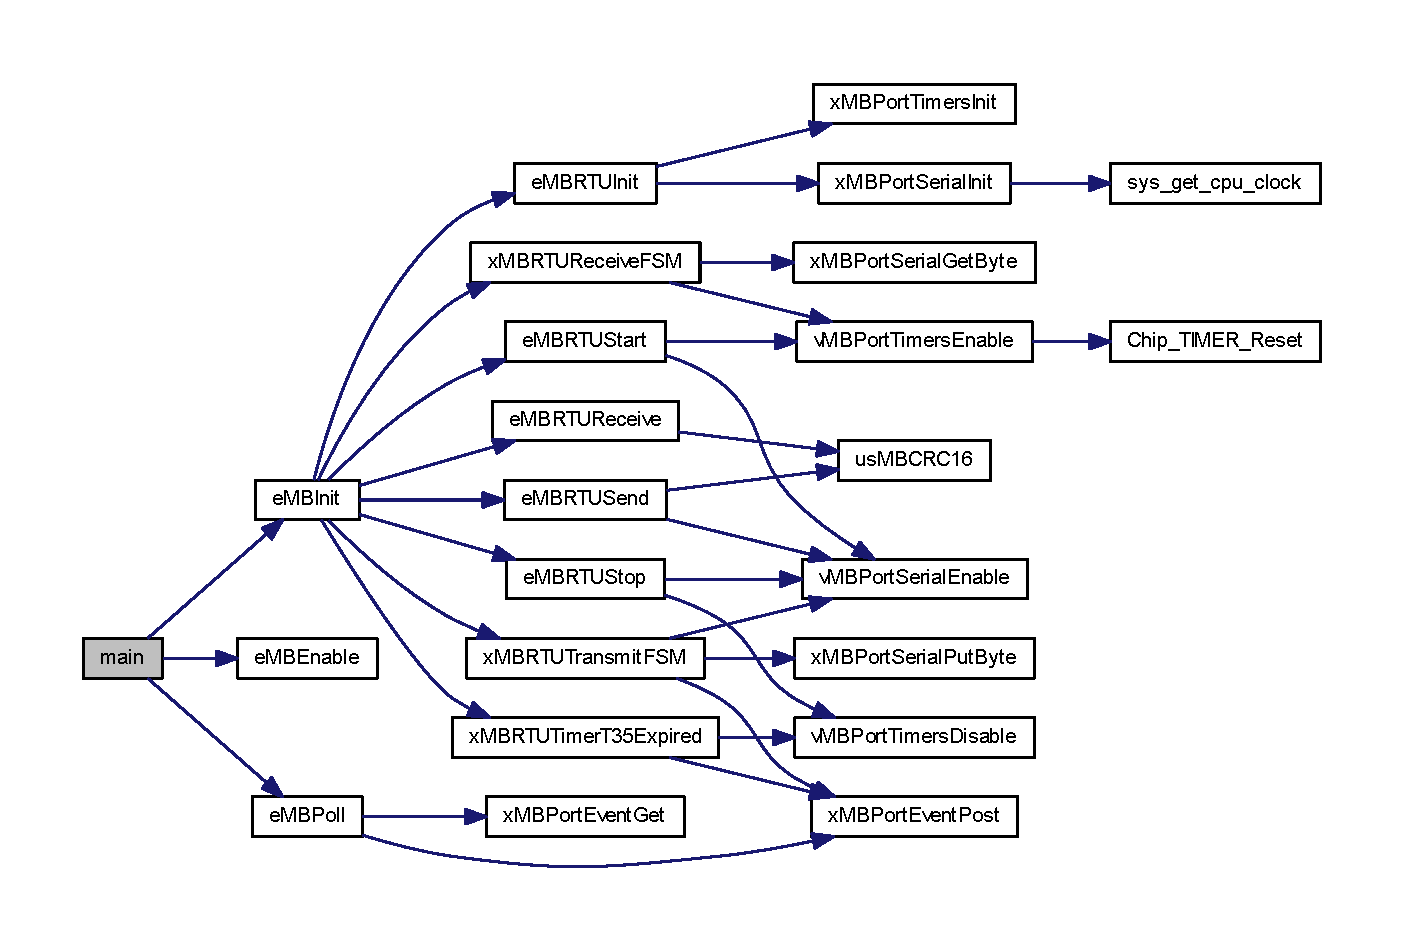
\includegraphics[width=350pt]{main_8c_a840291bc02cba5474a4cb46a9b9566fe_cgraph}
\end{center}
\end{figure}


\index{main.\+c@{main.\+c}!e\+M\+B\+Reg\+Input\+CB@{e\+M\+B\+Reg\+Input\+CB}}
\index{e\+M\+B\+Reg\+Input\+CB@{e\+M\+B\+Reg\+Input\+CB}!main.\+c@{main.\+c}}
\subsubsection[{\texorpdfstring{e\+M\+B\+Reg\+Input\+C\+B(\+U\+C\+H\+A\+R $\ast$puc\+Reg\+Buffer, U\+S\+H\+O\+R\+T us\+Address, U\+S\+H\+O\+R\+T us\+N\+Regs)}{eMBRegInputCB(UCHAR *pucRegBuffer, USHORT usAddress, USHORT usNRegs)}}]{\setlength{\rightskip}{0pt plus 5cm}e\+M\+B\+Error\+Code e\+M\+B\+Reg\+Input\+CB (
\begin{DoxyParamCaption}
\item[{U\+C\+H\+AR $\ast$}]{puc\+Reg\+Buffer, }
\item[{U\+S\+H\+O\+RT}]{us\+Address, }
\item[{U\+S\+H\+O\+RT}]{us\+N\+Regs}
\end{DoxyParamCaption}
)}\hypertarget{main_8c_a7816677520b1eb2ebecf15060a41bc81}{}\label{main_8c_a7816677520b1eb2ebecf15060a41bc81}


 \subsubsection*{e\+M\+B\+Reg\+Input\+CB }

Event Handler for G\+PI module \begin{DoxyVerb} @date                           DEC/02/2013
 @author                         FW_DEV_2
 @pre                            None
 @return                         None\end{DoxyVerb}
 

Definition at line 88 of file main.\+c.

\index{main.\+c@{main.\+c}!e\+M\+B\+Reg\+Holding\+CB@{e\+M\+B\+Reg\+Holding\+CB}}
\index{e\+M\+B\+Reg\+Holding\+CB@{e\+M\+B\+Reg\+Holding\+CB}!main.\+c@{main.\+c}}
\subsubsection[{\texorpdfstring{e\+M\+B\+Reg\+Holding\+C\+B(\+U\+C\+H\+A\+R $\ast$puc\+Reg\+Buffer, U\+S\+H\+O\+R\+T us\+Address, U\+S\+H\+O\+R\+T us\+N\+Regs, e\+M\+B\+Register\+Mode e\+Mode)}{eMBRegHoldingCB(UCHAR *pucRegBuffer, USHORT usAddress, USHORT usNRegs, eMBRegisterMode eMode)}}]{\setlength{\rightskip}{0pt plus 5cm}e\+M\+B\+Error\+Code e\+M\+B\+Reg\+Holding\+CB (
\begin{DoxyParamCaption}
\item[{U\+C\+H\+AR $\ast$}]{puc\+Reg\+Buffer, }
\item[{U\+S\+H\+O\+RT}]{us\+Address, }
\item[{U\+S\+H\+O\+RT}]{us\+N\+Regs, }
\item[{e\+M\+B\+Register\+Mode}]{e\+Mode}
\end{DoxyParamCaption}
)}\hypertarget{main_8c_a10d37e1d80224bf3b1eeb9e246d7582e}{}\label{main_8c_a10d37e1d80224bf3b1eeb9e246d7582e}


 \subsubsection*{e\+M\+B\+Reg\+Holding\+CB }

Event Handler for G\+PI module \begin{DoxyVerb} @date                           DEC/02/2013
 @author                         FW_DEV_2
 @pre                            None
 @return                         None\end{DoxyVerb}
 

Definition at line 126 of file main.\+c.

\index{main.\+c@{main.\+c}!e\+M\+B\+Reg\+Coils\+CB@{e\+M\+B\+Reg\+Coils\+CB}}
\index{e\+M\+B\+Reg\+Coils\+CB@{e\+M\+B\+Reg\+Coils\+CB}!main.\+c@{main.\+c}}
\subsubsection[{\texorpdfstring{e\+M\+B\+Reg\+Coils\+C\+B(\+U\+C\+H\+A\+R $\ast$puc\+Reg\+Buffer, U\+S\+H\+O\+R\+T us\+Address, U\+S\+H\+O\+R\+T us\+N\+Coils, e\+M\+B\+Register\+Mode e\+Mode)}{eMBRegCoilsCB(UCHAR *pucRegBuffer, USHORT usAddress, USHORT usNCoils, eMBRegisterMode eMode)}}]{\setlength{\rightskip}{0pt plus 5cm}e\+M\+B\+Error\+Code e\+M\+B\+Reg\+Coils\+CB (
\begin{DoxyParamCaption}
\item[{U\+C\+H\+AR $\ast$}]{puc\+Reg\+Buffer, }
\item[{U\+S\+H\+O\+RT}]{us\+Address, }
\item[{U\+S\+H\+O\+RT}]{us\+N\+Coils, }
\item[{e\+M\+B\+Register\+Mode}]{e\+Mode}
\end{DoxyParamCaption}
)}\hypertarget{main_8c_a88d9b719291515c60eee1bf9ffa1dd02}{}\label{main_8c_a88d9b719291515c60eee1bf9ffa1dd02}


 \subsubsection*{e\+M\+B\+Reg\+Coils\+CB }

Event Handler for G\+PI module \begin{DoxyVerb} @date                           DEC/02/2013
 @author                         FW_DEV_2
 @pre                            None
 @return                         None\end{DoxyVerb}
 

Definition at line 178 of file main.\+c.

\index{main.\+c@{main.\+c}!e\+M\+B\+Reg\+Discrete\+CB@{e\+M\+B\+Reg\+Discrete\+CB}}
\index{e\+M\+B\+Reg\+Discrete\+CB@{e\+M\+B\+Reg\+Discrete\+CB}!main.\+c@{main.\+c}}
\subsubsection[{\texorpdfstring{e\+M\+B\+Reg\+Discrete\+C\+B(\+U\+C\+H\+A\+R $\ast$puc\+Reg\+Buffer, U\+S\+H\+O\+R\+T us\+Address, U\+S\+H\+O\+R\+T us\+N\+Discrete)}{eMBRegDiscreteCB(UCHAR *pucRegBuffer, USHORT usAddress, USHORT usNDiscrete)}}]{\setlength{\rightskip}{0pt plus 5cm}e\+M\+B\+Error\+Code e\+M\+B\+Reg\+Discrete\+CB (
\begin{DoxyParamCaption}
\item[{U\+C\+H\+AR $\ast$}]{puc\+Reg\+Buffer, }
\item[{U\+S\+H\+O\+RT}]{us\+Address, }
\item[{U\+S\+H\+O\+RT}]{us\+N\+Discrete}
\end{DoxyParamCaption}
)}\hypertarget{main_8c_a38101f5da54af137e210a3b8b9fa3887}{}\label{main_8c_a38101f5da54af137e210a3b8b9fa3887}


 \subsubsection*{e\+M\+B\+Reg\+Discrete\+CB }

Event Handler for G\+PI module \begin{DoxyVerb} @date                           DEC/02/2013
 @author                         FW_DEV_2
 @pre                            None
 @return                         None\end{DoxyVerb}
 

Definition at line 195 of file main.\+c.


\hypertarget{mb_8c}{}\section{mb.\+c File Reference}
\label{mb_8c}\index{mb.\+c@{mb.\+c}}


This is main source file for G\+PI Module.  


{\ttfamily \#include \char`\"{}stdlib.\+h\char`\"{}}\\*
{\ttfamily \#include \char`\"{}string.\+h\char`\"{}}\\*
{\ttfamily \#include \char`\"{}port.\+h\char`\"{}}\\*
{\ttfamily \#include \char`\"{}mb.\+h\char`\"{}}\\*
{\ttfamily \#include \char`\"{}mbconfig.\+h\char`\"{}}\\*
{\ttfamily \#include \char`\"{}mbframe.\+h\char`\"{}}\\*
{\ttfamily \#include \char`\"{}mbproto.\+h\char`\"{}}\\*
{\ttfamily \#include \char`\"{}mbfunc.\+h\char`\"{}}\\*
{\ttfamily \#include \char`\"{}mbport.\+h\char`\"{}}\\*
Include dependency graph for mb.\+c\+:\nopagebreak
\begin{figure}[H]
\begin{center}
\leavevmode
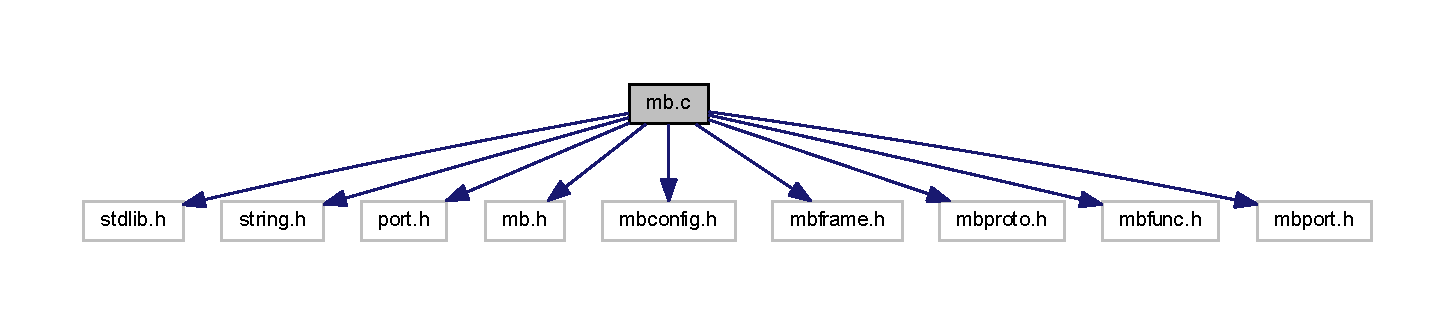
\includegraphics[width=350pt]{mb_8c__incl}
\end{center}
\end{figure}
\subsection*{Macros}
\begin{DoxyCompactItemize}
\item 
\#define {\bfseries M\+B\+\_\+\+P\+O\+R\+T\+\_\+\+H\+A\+S\+\_\+\+C\+L\+O\+SE}~0\hypertarget{mb_8c_a63c1fbefc04d96d29ef84407e22c4e3e}{}\label{mb_8c_a63c1fbefc04d96d29ef84407e22c4e3e}

\end{DoxyCompactItemize}
\subsection*{Enumerations}
\begin{DoxyCompactItemize}
\item 
enum \{ \\*
{\bfseries S\+T\+A\+T\+E\+\_\+\+E\+N\+A\+B\+L\+ED}, 
\\*
{\bfseries S\+T\+A\+T\+E\+\_\+\+D\+I\+S\+A\+B\+L\+ED}, 
\\*
{\bfseries S\+T\+A\+T\+E\+\_\+\+N\+O\+T\+\_\+\+I\+N\+I\+T\+I\+A\+L\+I\+Z\+ED}
 \}\hypertarget{mb_8c_a06fc87d81c62e9abb8790b6e5713c55b}{}\label{mb_8c_a06fc87d81c62e9abb8790b6e5713c55b}

\end{DoxyCompactItemize}
\subsection*{Functions}
\begin{DoxyCompactItemize}
\item 
e\+M\+B\+Error\+Code \hyperlink{mb_8c_a622dbe6b38ff1d255523d4736fa3da26}{e\+M\+B\+Init} (e\+M\+B\+Mode e\+Mode, U\+C\+H\+AR uc\+Slave\+Address, U\+C\+H\+AR uc\+Port, U\+L\+O\+NG ul\+Baud\+Rate, e\+M\+B\+Parity e\+Parity)
\item 
e\+M\+B\+Error\+Code \hyperlink{mb_8c_a5f6e66893b2388a602ac453253a00784}{e\+M\+B\+Register\+CB} (U\+C\+H\+AR uc\+Function\+Code, px\+M\+B\+Function\+Handler px\+Handler)
\item 
e\+M\+B\+Error\+Code \hyperlink{mb_8c_ac20080d92be2934456e2a5d27cd36310}{e\+M\+B\+Close} (void)
\item 
e\+M\+B\+Error\+Code \hyperlink{mb_8c_ab697be370833d562e6b016626d996132}{e\+M\+B\+Enable} (void)
\item 
e\+M\+B\+Error\+Code \hyperlink{mb_8c_abcc2a31ec41fc276ab3c3ac705defdf3}{e\+M\+B\+Disable} (void)
\item 
e\+M\+B\+Error\+Code \hyperlink{mb_8c_a12648c98d45f768ba878fbcee46caca5}{e\+M\+B\+Poll} (void)
\end{DoxyCompactItemize}
\subsection*{Variables}
\begin{DoxyCompactItemize}
\item 
B\+O\+OL($\ast$ {\bfseries px\+M\+B\+Frame\+C\+B\+Byte\+Received} )(void)\hypertarget{mb_8c_a4d1633f4b1d60cace408738c04fce911}{}\label{mb_8c_a4d1633f4b1d60cace408738c04fce911}

\item 
B\+O\+OL($\ast$ {\bfseries px\+M\+B\+Frame\+C\+B\+Transmitter\+Empty} )(void)\hypertarget{mb_8c_a019be320e5b288e526d4540b8f3b72fa}{}\label{mb_8c_a019be320e5b288e526d4540b8f3b72fa}

\item 
B\+O\+OL($\ast$ {\bfseries px\+M\+B\+Port\+C\+B\+Timer\+Expired} )(void)\hypertarget{mb_8c_a3b5983cb09b81183b03bea267a817980}{}\label{mb_8c_a3b5983cb09b81183b03bea267a817980}

\item 
B\+O\+OL($\ast$ {\bfseries px\+M\+B\+Frame\+C\+B\+Receive\+F\+S\+M\+Cur} )(void)\hypertarget{mb_8c_a3f01b620e5050996ae85dd49a1060ecb}{}\label{mb_8c_a3f01b620e5050996ae85dd49a1060ecb}

\item 
B\+O\+OL($\ast$ {\bfseries px\+M\+B\+Frame\+C\+B\+Transmit\+F\+S\+M\+Cur} )(void)\hypertarget{mb_8c_a78d9c464d5735a51451e8cc2a18e8568}{}\label{mb_8c_a78d9c464d5735a51451e8cc2a18e8568}

\end{DoxyCompactItemize}


\subsection{Detailed Description}
This is main source file for G\+PI Module. 

Free\+Modbus Libary\+: A portable Modbus implementation for Modbus A\+S\+C\+I\+I/\+R\+TU. Copyright (c) 2006 Christian Walter \href{mailto:wolti@sil.at}{\tt wolti@sil.\+at} All rights reserved.

Redistribution and use in source and binary forms, with or without modification, are permitted provided that the following conditions are met\+:
\begin{DoxyEnumerate}
\item Redistributions of source code must retain the above copyright notice, this list of conditions and the following disclaimer.
\item Redistributions in binary form must reproduce the above copyright notice, this list of conditions and the following disclaimer in the documentation and/or other materials provided with the distribution.
\item The name of the author may not be used to endorse or promote products derived from this software without specific prior written permission.
\end{DoxyEnumerate}

T\+H\+IS S\+O\+F\+T\+W\+A\+RE IS P\+R\+O\+V\+I\+D\+ED BY T\+HE A\+U\+T\+H\+OR ``\+AS IS\textquotesingle{}\textquotesingle{} A\+ND A\+NY E\+X\+P\+R\+E\+SS OR I\+M\+P\+L\+I\+ED W\+A\+R\+R\+A\+N\+T\+I\+ES, I\+N\+C\+L\+U\+D\+I\+NG, B\+UT N\+OT L\+I\+M\+I\+T\+ED TO, T\+HE I\+M\+P\+L\+I\+ED W\+A\+R\+R\+A\+N\+T\+I\+ES OF M\+E\+R\+C\+H\+A\+N\+T\+A\+B\+I\+L\+I\+TY A\+ND F\+I\+T\+N\+E\+SS F\+OR A P\+A\+R\+T\+I\+C\+U\+L\+AR P\+U\+R\+P\+O\+SE A\+RE D\+I\+S\+C\+L\+A\+I\+M\+ED. IN NO E\+V\+E\+NT S\+H\+A\+LL T\+HE A\+U\+T\+H\+OR BE L\+I\+A\+B\+LE F\+OR A\+NY D\+I\+R\+E\+CT, I\+N\+D\+I\+R\+E\+CT, I\+N\+C\+I\+D\+E\+N\+T\+AL, S\+P\+E\+C\+I\+AL, E\+X\+E\+M\+P\+L\+A\+RY, OR C\+O\+N\+S\+E\+Q\+U\+E\+N\+T\+I\+AL D\+A\+M\+A\+G\+ES (I\+N\+C\+L\+U\+D\+I\+NG, B\+UT N\+OT L\+I\+M\+I\+T\+ED TO, P\+R\+O\+C\+U\+R\+E\+M\+E\+NT OF S\+U\+B\+S\+T\+I\+T\+U\+TE G\+O\+O\+DS OR S\+E\+R\+V\+I\+C\+ES; L\+O\+SS OF U\+SE, D\+A\+TA, OR P\+R\+O\+F\+I\+TS; OR B\+U\+S\+I\+N\+E\+SS I\+N\+T\+E\+R\+R\+U\+P\+T\+I\+ON) H\+O\+W\+E\+V\+ER C\+A\+U\+S\+ED A\+ND ON A\+NY T\+H\+E\+O\+RY OF L\+I\+A\+B\+I\+L\+I\+TY, W\+H\+E\+T\+H\+ER IN C\+O\+N\+T\+R\+A\+CT, S\+T\+R\+I\+CT L\+I\+A\+B\+I\+L\+I\+TY, OR T\+O\+RT (I\+N\+C\+L\+U\+D\+I\+NG N\+E\+G\+L\+I\+G\+E\+N\+CE OR O\+T\+H\+E\+R\+W\+I\+SE) A\+R\+I\+S\+I\+NG IN A\+NY W\+AY O\+UT OF T\+HE U\+SE OF T\+H\+IS S\+O\+F\+T\+W\+A\+RE, E\+V\+EN IF A\+D\+V\+I\+S\+ED OF T\+HE P\+O\+S\+S\+I\+B\+I\+L\+I\+TY OF S\+U\+CH D\+A\+M\+A\+GE.

File\+: \begin{DoxyParagraph}{Id}
\hyperlink{mb_8c}{mb.\+c},v 1.\+27 2007/02/18 23\+:45\+:41 wolti Exp 
\end{DoxyParagraph}


\subsection{Function Documentation}
\index{mb.\+c@{mb.\+c}!e\+M\+B\+Init@{e\+M\+B\+Init}}
\index{e\+M\+B\+Init@{e\+M\+B\+Init}!mb.\+c@{mb.\+c}}
\subsubsection[{\texorpdfstring{e\+M\+B\+Init(e\+M\+B\+Mode e\+Mode, U\+C\+H\+A\+R uc\+Slave\+Address, U\+C\+H\+A\+R uc\+Port, U\+L\+O\+N\+G ul\+Baud\+Rate, e\+M\+B\+Parity e\+Parity)}{eMBInit(eMBMode eMode, UCHAR ucSlaveAddress, UCHAR ucPort, ULONG ulBaudRate, eMBParity eParity)}}]{\setlength{\rightskip}{0pt plus 5cm}e\+M\+B\+Error\+Code e\+M\+B\+Init (
\begin{DoxyParamCaption}
\item[{e\+M\+B\+Mode}]{e\+Mode, }
\item[{U\+C\+H\+AR}]{uc\+Slave\+Address, }
\item[{U\+C\+H\+AR}]{uc\+Port, }
\item[{U\+L\+O\+NG}]{ul\+Baud\+Rate, }
\item[{e\+M\+B\+Parity}]{e\+Parity}
\end{DoxyParamCaption}
)}\hypertarget{mb_8c_a622dbe6b38ff1d255523d4736fa3da26}{}\label{mb_8c_a622dbe6b38ff1d255523d4736fa3da26}


 \subsubsection*{e\+M\+B\+Init }

Event Handler for G\+PI module \begin{DoxyVerb} @date                           DEC/02/2013
 @author                         FW_DEV_2
 @pre                            None
 @return                         None\end{DoxyVerb}
 

Definition at line 143 of file mb.\+c.



Here is the call graph for this function\+:
\nopagebreak
\begin{figure}[H]
\begin{center}
\leavevmode
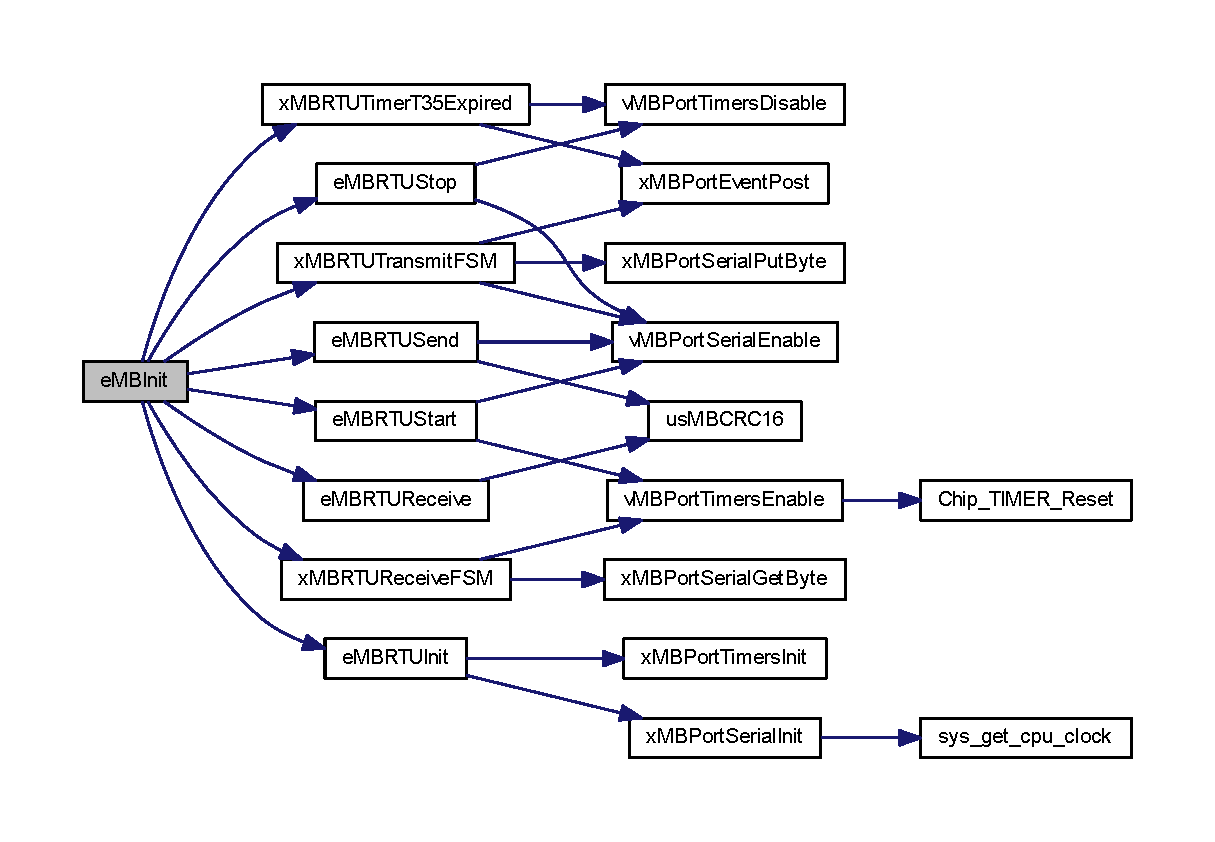
\includegraphics[width=350pt]{mb_8c_a622dbe6b38ff1d255523d4736fa3da26_cgraph}
\end{center}
\end{figure}




Here is the caller graph for this function\+:
\nopagebreak
\begin{figure}[H]
\begin{center}
\leavevmode
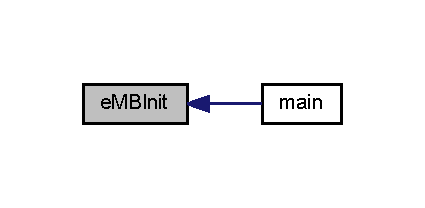
\includegraphics[width=204pt]{mb_8c_a622dbe6b38ff1d255523d4736fa3da26_icgraph}
\end{center}
\end{figure}


\index{mb.\+c@{mb.\+c}!e\+M\+B\+Register\+CB@{e\+M\+B\+Register\+CB}}
\index{e\+M\+B\+Register\+CB@{e\+M\+B\+Register\+CB}!mb.\+c@{mb.\+c}}
\subsubsection[{\texorpdfstring{e\+M\+B\+Register\+C\+B(\+U\+C\+H\+A\+R uc\+Function\+Code, px\+M\+B\+Function\+Handler px\+Handler)}{eMBRegisterCB(UCHAR ucFunctionCode, pxMBFunctionHandler pxHandler)}}]{\setlength{\rightskip}{0pt plus 5cm}e\+M\+B\+Error\+Code e\+M\+B\+Register\+CB (
\begin{DoxyParamCaption}
\item[{U\+C\+H\+AR}]{uc\+Function\+Code, }
\item[{px\+M\+B\+Function\+Handler}]{px\+Handler}
\end{DoxyParamCaption}
)}\hypertarget{mb_8c_a5f6e66893b2388a602ac453253a00784}{}\label{mb_8c_a5f6e66893b2388a602ac453253a00784}


 \subsubsection*{e\+M\+B\+Register\+CB }

Event Handler for G\+PI module \begin{DoxyVerb} @date                           DEC/02/2013
 @author                         FW_DEV_2
 @pre                            None
 @return                         None\end{DoxyVerb}
 

Definition at line 244 of file mb.\+c.

\index{mb.\+c@{mb.\+c}!e\+M\+B\+Close@{e\+M\+B\+Close}}
\index{e\+M\+B\+Close@{e\+M\+B\+Close}!mb.\+c@{mb.\+c}}
\subsubsection[{\texorpdfstring{e\+M\+B\+Close(void)}{eMBClose(void)}}]{\setlength{\rightskip}{0pt plus 5cm}e\+M\+B\+Error\+Code e\+M\+B\+Close (
\begin{DoxyParamCaption}
\item[{void}]{}
\end{DoxyParamCaption}
)}\hypertarget{mb_8c_ac20080d92be2934456e2a5d27cd36310}{}\label{mb_8c_ac20080d92be2934456e2a5d27cd36310}


 \subsubsection*{e\+M\+B\+Close }

Event Handler for G\+PI module \begin{DoxyVerb} @date                           DEC/02/2013
 @author                         FW_DEV_2
 @pre                            None
 @return                         None\end{DoxyVerb}
 

Definition at line 302 of file mb.\+c.

\index{mb.\+c@{mb.\+c}!e\+M\+B\+Enable@{e\+M\+B\+Enable}}
\index{e\+M\+B\+Enable@{e\+M\+B\+Enable}!mb.\+c@{mb.\+c}}
\subsubsection[{\texorpdfstring{e\+M\+B\+Enable(void)}{eMBEnable(void)}}]{\setlength{\rightskip}{0pt plus 5cm}e\+M\+B\+Error\+Code e\+M\+B\+Enable (
\begin{DoxyParamCaption}
\item[{void}]{}
\end{DoxyParamCaption}
)}\hypertarget{mb_8c_ab697be370833d562e6b016626d996132}{}\label{mb_8c_ab697be370833d562e6b016626d996132}


 \subsubsection*{e\+M\+B\+Enable }

Event Handler for G\+PI module \begin{DoxyVerb} @date                           DEC/02/2013
 @author                         FW_DEV_2
 @pre                            None
 @return                         None\end{DoxyVerb}
 

Definition at line 332 of file mb.\+c.



Here is the caller graph for this function\+:
\nopagebreak
\begin{figure}[H]
\begin{center}
\leavevmode
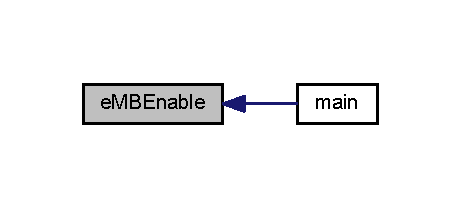
\includegraphics[width=221pt]{mb_8c_ab697be370833d562e6b016626d996132_icgraph}
\end{center}
\end{figure}


\index{mb.\+c@{mb.\+c}!e\+M\+B\+Disable@{e\+M\+B\+Disable}}
\index{e\+M\+B\+Disable@{e\+M\+B\+Disable}!mb.\+c@{mb.\+c}}
\subsubsection[{\texorpdfstring{e\+M\+B\+Disable(void)}{eMBDisable(void)}}]{\setlength{\rightskip}{0pt plus 5cm}e\+M\+B\+Error\+Code e\+M\+B\+Disable (
\begin{DoxyParamCaption}
\item[{void}]{}
\end{DoxyParamCaption}
)}\hypertarget{mb_8c_abcc2a31ec41fc276ab3c3ac705defdf3}{}\label{mb_8c_abcc2a31ec41fc276ab3c3ac705defdf3}


 \subsubsection*{e\+M\+B\+Disable }

Event Handler for G\+PI module \begin{DoxyVerb} @date                           DEC/02/2013
 @author                         FW_DEV_2
 @pre                            None
 @return                         None\end{DoxyVerb}
 

Definition at line 361 of file mb.\+c.

\index{mb.\+c@{mb.\+c}!e\+M\+B\+Poll@{e\+M\+B\+Poll}}
\index{e\+M\+B\+Poll@{e\+M\+B\+Poll}!mb.\+c@{mb.\+c}}
\subsubsection[{\texorpdfstring{e\+M\+B\+Poll(void)}{eMBPoll(void)}}]{\setlength{\rightskip}{0pt plus 5cm}e\+M\+B\+Error\+Code e\+M\+B\+Poll (
\begin{DoxyParamCaption}
\item[{void}]{}
\end{DoxyParamCaption}
)}\hypertarget{mb_8c_a12648c98d45f768ba878fbcee46caca5}{}\label{mb_8c_a12648c98d45f768ba878fbcee46caca5}


 \subsubsection*{e\+M\+B\+Poll }

Event Handler for G\+PI module \begin{DoxyVerb} @date                           DEC/02/2013
 @author                         FW_DEV_2
 @pre                            None
 @return                         None\end{DoxyVerb}
 

Definition at line 394 of file mb.\+c.



Here is the call graph for this function\+:
\nopagebreak
\begin{figure}[H]
\begin{center}
\leavevmode
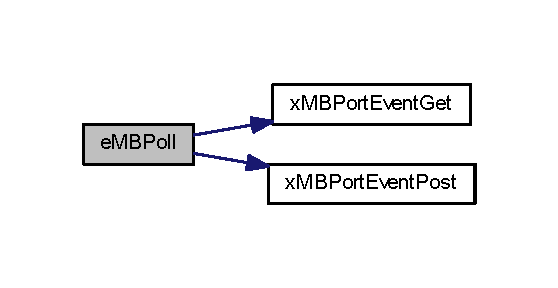
\includegraphics[width=268pt]{mb_8c_a12648c98d45f768ba878fbcee46caca5_cgraph}
\end{center}
\end{figure}




Here is the caller graph for this function\+:
\nopagebreak
\begin{figure}[H]
\begin{center}
\leavevmode
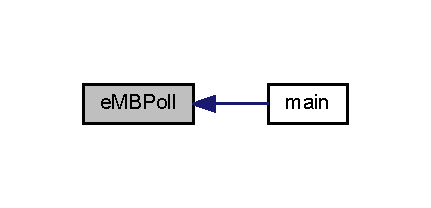
\includegraphics[width=207pt]{mb_8c_a12648c98d45f768ba878fbcee46caca5_icgraph}
\end{center}
\end{figure}



\hypertarget{mbcrc_8c}{}\section{mbcrc.\+c File Reference}
\label{mbcrc_8c}\index{mbcrc.\+c@{mbcrc.\+c}}
{\ttfamily \#include \char`\"{}port.\+h\char`\"{}}\\*
Include dependency graph for mbcrc.\+c\+:
\nopagebreak
\begin{figure}[H]
\begin{center}
\leavevmode
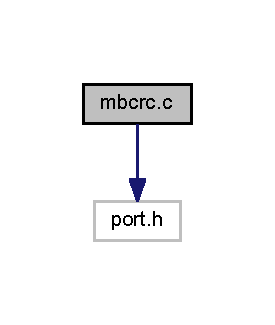
\includegraphics[width=132pt]{mbcrc_8c__incl}
\end{center}
\end{figure}
\subsection*{Functions}
\begin{DoxyCompactItemize}
\item 
U\+S\+H\+O\+RT \hyperlink{mbcrc_8c_abc48f359fd99e303016c8b74cc82c3ff}{us\+M\+B\+C\+R\+C16} (U\+C\+H\+AR $\ast$puc\+Frame, U\+S\+H\+O\+RT us\+Len)
\end{DoxyCompactItemize}


\subsection{Detailed Description}
Free\+Modbus Libary\+: A portable Modbus implementation for Modbus A\+S\+C\+I\+I/\+R\+TU. Copyright (c) 2006 Christian Walter \href{mailto:wolti@sil.at}{\tt wolti@sil.\+at} All rights reserved.

Redistribution and use in source and binary forms, with or without modification, are permitted provided that the following conditions are met\+:
\begin{DoxyEnumerate}
\item Redistributions of source code must retain the above copyright notice, this list of conditions and the following disclaimer.
\item Redistributions in binary form must reproduce the above copyright notice, this list of conditions and the following disclaimer in the documentation and/or other materials provided with the distribution.
\item The name of the author may not be used to endorse or promote products derived from this software without specific prior written permission.
\end{DoxyEnumerate}

T\+H\+IS S\+O\+F\+T\+W\+A\+RE IS P\+R\+O\+V\+I\+D\+ED BY T\+HE A\+U\+T\+H\+OR ``\+AS IS\textquotesingle{}\textquotesingle{} A\+ND A\+NY E\+X\+P\+R\+E\+SS OR I\+M\+P\+L\+I\+ED W\+A\+R\+R\+A\+N\+T\+I\+ES, I\+N\+C\+L\+U\+D\+I\+NG, B\+UT N\+OT L\+I\+M\+I\+T\+ED TO, T\+HE I\+M\+P\+L\+I\+ED W\+A\+R\+R\+A\+N\+T\+I\+ES OF M\+E\+R\+C\+H\+A\+N\+T\+A\+B\+I\+L\+I\+TY A\+ND F\+I\+T\+N\+E\+SS F\+OR A P\+A\+R\+T\+I\+C\+U\+L\+AR P\+U\+R\+P\+O\+SE A\+RE D\+I\+S\+C\+L\+A\+I\+M\+ED. IN NO E\+V\+E\+NT S\+H\+A\+LL T\+HE A\+U\+T\+H\+OR BE L\+I\+A\+B\+LE F\+OR A\+NY D\+I\+R\+E\+CT, I\+N\+D\+I\+R\+E\+CT, I\+N\+C\+I\+D\+E\+N\+T\+AL, S\+P\+E\+C\+I\+AL, E\+X\+E\+M\+P\+L\+A\+RY, OR C\+O\+N\+S\+E\+Q\+U\+E\+N\+T\+I\+AL D\+A\+M\+A\+G\+ES (I\+N\+C\+L\+U\+D\+I\+NG, B\+UT N\+OT L\+I\+M\+I\+T\+ED TO, P\+R\+O\+C\+U\+R\+E\+M\+E\+NT OF S\+U\+B\+S\+T\+I\+T\+U\+TE G\+O\+O\+DS OR S\+E\+R\+V\+I\+C\+ES; L\+O\+SS OF U\+SE, D\+A\+TA, OR P\+R\+O\+F\+I\+TS; OR B\+U\+S\+I\+N\+E\+SS I\+N\+T\+E\+R\+R\+U\+P\+T\+I\+ON) H\+O\+W\+E\+V\+ER C\+A\+U\+S\+ED A\+ND ON A\+NY T\+H\+E\+O\+RY OF L\+I\+A\+B\+I\+L\+I\+TY, W\+H\+E\+T\+H\+ER IN C\+O\+N\+T\+R\+A\+CT, S\+T\+R\+I\+CT L\+I\+A\+B\+I\+L\+I\+TY, OR T\+O\+RT (I\+N\+C\+L\+U\+D\+I\+NG N\+E\+G\+L\+I\+G\+E\+N\+CE OR O\+T\+H\+E\+R\+W\+I\+SE) A\+R\+I\+S\+I\+NG IN A\+NY W\+AY O\+UT OF T\+HE U\+SE OF T\+H\+IS S\+O\+F\+T\+W\+A\+RE, E\+V\+EN IF A\+D\+V\+I\+S\+ED OF T\+HE P\+O\+S\+S\+I\+B\+I\+L\+I\+TY OF S\+U\+CH D\+A\+M\+A\+GE.

File\+: \begin{DoxyParagraph}{Id}
\hyperlink{mbcrc_8c}{mbcrc.\+c},v 1.\+7 2007/02/18 23\+:50\+:27 wolti Exp 
\end{DoxyParagraph}


\subsection{Function Documentation}
\index{mbcrc.\+c@{mbcrc.\+c}!us\+M\+B\+C\+R\+C16@{us\+M\+B\+C\+R\+C16}}
\index{us\+M\+B\+C\+R\+C16@{us\+M\+B\+C\+R\+C16}!mbcrc.\+c@{mbcrc.\+c}}
\subsubsection[{\texorpdfstring{us\+M\+B\+C\+R\+C16(\+U\+C\+H\+A\+R $\ast$puc\+Frame, U\+S\+H\+O\+R\+T us\+Len)}{usMBCRC16(UCHAR *pucFrame, USHORT usLen)}}]{\setlength{\rightskip}{0pt plus 5cm}U\+S\+H\+O\+RT us\+M\+B\+C\+R\+C16 (
\begin{DoxyParamCaption}
\item[{U\+C\+H\+AR $\ast$}]{puc\+Frame, }
\item[{U\+S\+H\+O\+RT}]{us\+Len}
\end{DoxyParamCaption}
)}\hypertarget{mbcrc_8c_abc48f359fd99e303016c8b74cc82c3ff}{}\label{mbcrc_8c_abc48f359fd99e303016c8b74cc82c3ff}


 \subsubsection*{us\+M\+B\+C\+R\+C16 }

Event Handler for G\+PI module \begin{DoxyVerb} @date                           DEC/02/2013
 @author                         FW_DEV_2
 @pre                            None
 @return                         None\end{DoxyVerb}
 

Definition at line 97 of file mbcrc.\+c.



Here is the caller graph for this function\+:
\nopagebreak
\begin{figure}[H]
\begin{center}
\leavevmode
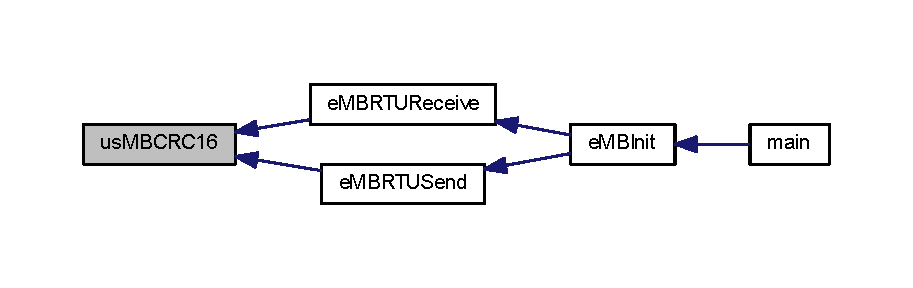
\includegraphics[width=350pt]{mbcrc_8c_abc48f359fd99e303016c8b74cc82c3ff_icgraph}
\end{center}
\end{figure}



\hypertarget{mbfunccoils_8c}{}\section{mbfunccoils.\+c File Reference}
\label{mbfunccoils_8c}\index{mbfunccoils.\+c@{mbfunccoils.\+c}}
{\ttfamily \#include \char`\"{}stdlib.\+h\char`\"{}}\\*
{\ttfamily \#include \char`\"{}string.\+h\char`\"{}}\\*
{\ttfamily \#include \char`\"{}port.\+h\char`\"{}}\\*
{\ttfamily \#include \char`\"{}mb.\+h\char`\"{}}\\*
{\ttfamily \#include \char`\"{}mbframe.\+h\char`\"{}}\\*
{\ttfamily \#include \char`\"{}mbproto.\+h\char`\"{}}\\*
{\ttfamily \#include \char`\"{}mbconfig.\+h\char`\"{}}\\*
Include dependency graph for mbfunccoils.\+c\+:
\nopagebreak
\begin{figure}[H]
\begin{center}
\leavevmode
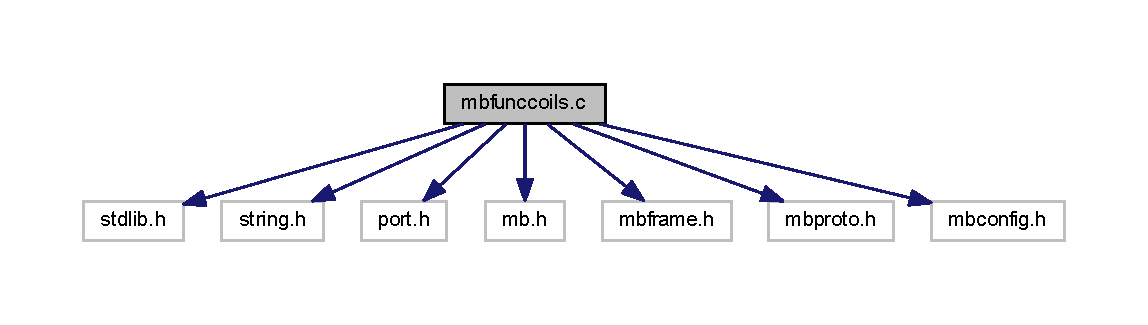
\includegraphics[width=350pt]{mbfunccoils_8c__incl}
\end{center}
\end{figure}
\subsection*{Macros}
\begin{DoxyCompactItemize}
\item 
\#define {\bfseries M\+B\+\_\+\+P\+D\+U\+\_\+\+F\+U\+N\+C\+\_\+\+R\+E\+A\+D\+\_\+\+A\+D\+D\+R\+\_\+\+O\+FF}~( M\+B\+\_\+\+P\+D\+U\+\_\+\+D\+A\+T\+A\+\_\+\+O\+FF )\hypertarget{mbfunccoils_8c_ab3c4b5bd48b2160671541e4026f2caae}{}\label{mbfunccoils_8c_ab3c4b5bd48b2160671541e4026f2caae}

\item 
\#define {\bfseries M\+B\+\_\+\+P\+D\+U\+\_\+\+F\+U\+N\+C\+\_\+\+R\+E\+A\+D\+\_\+\+C\+O\+I\+L\+C\+N\+T\+\_\+\+O\+FF}~( M\+B\+\_\+\+P\+D\+U\+\_\+\+D\+A\+T\+A\+\_\+\+O\+FF + 2 )\hypertarget{mbfunccoils_8c_aa5c2152c1dedaf85596395824b7ca7a9}{}\label{mbfunccoils_8c_aa5c2152c1dedaf85596395824b7ca7a9}

\item 
\#define {\bfseries M\+B\+\_\+\+P\+D\+U\+\_\+\+F\+U\+N\+C\+\_\+\+R\+E\+A\+D\+\_\+\+S\+I\+ZE}~( 4 )\hypertarget{mbfunccoils_8c_a968555f75801294753a5b2da91bea764}{}\label{mbfunccoils_8c_a968555f75801294753a5b2da91bea764}

\item 
\#define {\bfseries M\+B\+\_\+\+P\+D\+U\+\_\+\+F\+U\+N\+C\+\_\+\+R\+E\+A\+D\+\_\+\+C\+O\+I\+L\+C\+N\+T\+\_\+\+M\+AX}~( 0x07\+D0 )\hypertarget{mbfunccoils_8c_a76ddc47804210a5c6a7cd159d4f851e1}{}\label{mbfunccoils_8c_a76ddc47804210a5c6a7cd159d4f851e1}

\item 
\#define {\bfseries M\+B\+\_\+\+P\+D\+U\+\_\+\+F\+U\+N\+C\+\_\+\+W\+R\+I\+T\+E\+\_\+\+A\+D\+D\+R\+\_\+\+O\+FF}~( M\+B\+\_\+\+P\+D\+U\+\_\+\+D\+A\+T\+A\+\_\+\+O\+FF )\hypertarget{mbfunccoils_8c_a7e062d894a248db85a8270050f94e97e}{}\label{mbfunccoils_8c_a7e062d894a248db85a8270050f94e97e}

\item 
\#define {\bfseries M\+B\+\_\+\+P\+D\+U\+\_\+\+F\+U\+N\+C\+\_\+\+W\+R\+I\+T\+E\+\_\+\+V\+A\+L\+U\+E\+\_\+\+O\+FF}~( M\+B\+\_\+\+P\+D\+U\+\_\+\+D\+A\+T\+A\+\_\+\+O\+FF + 2 )\hypertarget{mbfunccoils_8c_a3366487f1f94813dbf7e118146fe0698}{}\label{mbfunccoils_8c_a3366487f1f94813dbf7e118146fe0698}

\item 
\#define {\bfseries M\+B\+\_\+\+P\+D\+U\+\_\+\+F\+U\+N\+C\+\_\+\+W\+R\+I\+T\+E\+\_\+\+S\+I\+ZE}~( 4 )\hypertarget{mbfunccoils_8c_a740439a1794d2f5be18109f38be50862}{}\label{mbfunccoils_8c_a740439a1794d2f5be18109f38be50862}

\item 
\#define {\bfseries M\+B\+\_\+\+P\+D\+U\+\_\+\+F\+U\+N\+C\+\_\+\+W\+R\+I\+T\+E\+\_\+\+M\+U\+L\+\_\+\+A\+D\+D\+R\+\_\+\+O\+FF}~( M\+B\+\_\+\+P\+D\+U\+\_\+\+D\+A\+T\+A\+\_\+\+O\+FF )\hypertarget{mbfunccoils_8c_ac28b968f1b4bbba124a7576e89a4ee96}{}\label{mbfunccoils_8c_ac28b968f1b4bbba124a7576e89a4ee96}

\item 
\#define {\bfseries M\+B\+\_\+\+P\+D\+U\+\_\+\+F\+U\+N\+C\+\_\+\+W\+R\+I\+T\+E\+\_\+\+M\+U\+L\+\_\+\+C\+O\+I\+L\+C\+N\+T\+\_\+\+O\+FF}~( M\+B\+\_\+\+P\+D\+U\+\_\+\+D\+A\+T\+A\+\_\+\+O\+FF + 2 )\hypertarget{mbfunccoils_8c_a68b2c3c056ee85f7c00030fe7500724a}{}\label{mbfunccoils_8c_a68b2c3c056ee85f7c00030fe7500724a}

\item 
\#define {\bfseries M\+B\+\_\+\+P\+D\+U\+\_\+\+F\+U\+N\+C\+\_\+\+W\+R\+I\+T\+E\+\_\+\+M\+U\+L\+\_\+\+B\+Y\+T\+E\+C\+N\+T\+\_\+\+O\+FF}~( M\+B\+\_\+\+P\+D\+U\+\_\+\+D\+A\+T\+A\+\_\+\+O\+FF + 4 )\hypertarget{mbfunccoils_8c_ad40dd5916e0b4785402f5f583a288035}{}\label{mbfunccoils_8c_ad40dd5916e0b4785402f5f583a288035}

\item 
\#define {\bfseries M\+B\+\_\+\+P\+D\+U\+\_\+\+F\+U\+N\+C\+\_\+\+W\+R\+I\+T\+E\+\_\+\+M\+U\+L\+\_\+\+V\+A\+L\+U\+E\+S\+\_\+\+O\+FF}~( M\+B\+\_\+\+P\+D\+U\+\_\+\+D\+A\+T\+A\+\_\+\+O\+FF + 5 )\hypertarget{mbfunccoils_8c_a712155f8f2d0babedfa33f63a07e875b}{}\label{mbfunccoils_8c_a712155f8f2d0babedfa33f63a07e875b}

\item 
\#define {\bfseries M\+B\+\_\+\+P\+D\+U\+\_\+\+F\+U\+N\+C\+\_\+\+W\+R\+I\+T\+E\+\_\+\+M\+U\+L\+\_\+\+S\+I\+Z\+E\+\_\+\+M\+IN}~( 5 )\hypertarget{mbfunccoils_8c_a2e813e9e8d7743a9ae3f57bed67d0f64}{}\label{mbfunccoils_8c_a2e813e9e8d7743a9ae3f57bed67d0f64}

\item 
\#define {\bfseries M\+B\+\_\+\+P\+D\+U\+\_\+\+F\+U\+N\+C\+\_\+\+W\+R\+I\+T\+E\+\_\+\+M\+U\+L\+\_\+\+C\+O\+I\+L\+C\+N\+T\+\_\+\+M\+AX}~( 0x07\+B0 )\hypertarget{mbfunccoils_8c_aab9b5eb819556c0dbd8d0077cd167cc2}{}\label{mbfunccoils_8c_aab9b5eb819556c0dbd8d0077cd167cc2}

\end{DoxyCompactItemize}
\subsection*{Functions}
\begin{DoxyCompactItemize}
\item 
e\+M\+B\+Exception \hyperlink{mbfunccoils_8c_ad5d2cc07a83fa7ea723ed734c905bc55}{prve\+M\+B\+Error2\+Exception} (e\+M\+B\+Error\+Code e\+Error\+Code)
\end{DoxyCompactItemize}


\subsection{Detailed Description}
Free\+Modbus Libary\+: A portable Modbus implementation for Modbus A\+S\+C\+I\+I/\+R\+TU. Copyright (c) 2006 Christian Walter \href{mailto:wolti@sil.at}{\tt wolti@sil.\+at} All rights reserved.

Redistribution and use in source and binary forms, with or without modification, are permitted provided that the following conditions are met\+:
\begin{DoxyEnumerate}
\item Redistributions of source code must retain the above copyright notice, this list of conditions and the following disclaimer.
\item Redistributions in binary form must reproduce the above copyright notice, this list of conditions and the following disclaimer in the documentation and/or other materials provided with the distribution.
\item The name of the author may not be used to endorse or promote products derived from this software without specific prior written permission.
\end{DoxyEnumerate}

T\+H\+IS S\+O\+F\+T\+W\+A\+RE IS P\+R\+O\+V\+I\+D\+ED BY T\+HE A\+U\+T\+H\+OR ``\+AS IS\textquotesingle{}\textquotesingle{} A\+ND A\+NY E\+X\+P\+R\+E\+SS OR I\+M\+P\+L\+I\+ED W\+A\+R\+R\+A\+N\+T\+I\+ES, I\+N\+C\+L\+U\+D\+I\+NG, B\+UT N\+OT L\+I\+M\+I\+T\+ED TO, T\+HE I\+M\+P\+L\+I\+ED W\+A\+R\+R\+A\+N\+T\+I\+ES OF M\+E\+R\+C\+H\+A\+N\+T\+A\+B\+I\+L\+I\+TY A\+ND F\+I\+T\+N\+E\+SS F\+OR A P\+A\+R\+T\+I\+C\+U\+L\+AR P\+U\+R\+P\+O\+SE A\+RE D\+I\+S\+C\+L\+A\+I\+M\+ED. IN NO E\+V\+E\+NT S\+H\+A\+LL T\+HE A\+U\+T\+H\+OR BE L\+I\+A\+B\+LE F\+OR A\+NY D\+I\+R\+E\+CT, I\+N\+D\+I\+R\+E\+CT, I\+N\+C\+I\+D\+E\+N\+T\+AL, S\+P\+E\+C\+I\+AL, E\+X\+E\+M\+P\+L\+A\+RY, OR C\+O\+N\+S\+E\+Q\+U\+E\+N\+T\+I\+AL D\+A\+M\+A\+G\+ES (I\+N\+C\+L\+U\+D\+I\+NG, B\+UT N\+OT L\+I\+M\+I\+T\+ED TO, P\+R\+O\+C\+U\+R\+E\+M\+E\+NT OF S\+U\+B\+S\+T\+I\+T\+U\+TE G\+O\+O\+DS OR S\+E\+R\+V\+I\+C\+ES; L\+O\+SS OF U\+SE, D\+A\+TA, OR P\+R\+O\+F\+I\+TS; OR B\+U\+S\+I\+N\+E\+SS I\+N\+T\+E\+R\+R\+U\+P\+T\+I\+ON) H\+O\+W\+E\+V\+ER C\+A\+U\+S\+ED A\+ND ON A\+NY T\+H\+E\+O\+RY OF L\+I\+A\+B\+I\+L\+I\+TY, W\+H\+E\+T\+H\+ER IN C\+O\+N\+T\+R\+A\+CT, S\+T\+R\+I\+CT L\+I\+A\+B\+I\+L\+I\+TY, OR T\+O\+RT (I\+N\+C\+L\+U\+D\+I\+NG N\+E\+G\+L\+I\+G\+E\+N\+CE OR O\+T\+H\+E\+R\+W\+I\+SE) A\+R\+I\+S\+I\+NG IN A\+NY W\+AY O\+UT OF T\+HE U\+SE OF T\+H\+IS S\+O\+F\+T\+W\+A\+RE, E\+V\+EN IF A\+D\+V\+I\+S\+ED OF T\+HE P\+O\+S\+S\+I\+B\+I\+L\+I\+TY OF S\+U\+CH D\+A\+M\+A\+GE.

File\+: \begin{DoxyParagraph}{Id}
\hyperlink{mbfunccoils_8c}{mbfunccoils.\+c},v 1.\+8 2007/02/18 23\+:47\+:16 wolti Exp 
\end{DoxyParagraph}


\subsection{Function Documentation}
\index{mbfunccoils.\+c@{mbfunccoils.\+c}!prve\+M\+B\+Error2\+Exception@{prve\+M\+B\+Error2\+Exception}}
\index{prve\+M\+B\+Error2\+Exception@{prve\+M\+B\+Error2\+Exception}!mbfunccoils.\+c@{mbfunccoils.\+c}}
\subsubsection[{\texorpdfstring{prve\+M\+B\+Error2\+Exception(e\+M\+B\+Error\+Code e\+Error\+Code)}{prveMBError2Exception(eMBErrorCode eErrorCode)}}]{\setlength{\rightskip}{0pt plus 5cm}e\+M\+B\+Exception prve\+M\+B\+Error2\+Exception (
\begin{DoxyParamCaption}
\item[{e\+M\+B\+Error\+Code}]{e\+Error\+Code}
\end{DoxyParamCaption}
)}\hypertarget{mbfunccoils_8c_ad5d2cc07a83fa7ea723ed734c905bc55}{}\label{mbfunccoils_8c_ad5d2cc07a83fa7ea723ed734c905bc55}


 \subsubsection*{prve\+M\+B\+Error2\+Exception }

Event Handler for G\+PI module \begin{DoxyVerb} @date                           DEC/02/2013
 @author                         FW_DEV_2
 @pre                            None
 @return                         None\end{DoxyVerb}
 

Definition at line 249 of file mbutils.\+c.


\hypertarget{mbfuncdisc_8c}{}\section{mbfuncdisc.\+c File Reference}
\label{mbfuncdisc_8c}\index{mbfuncdisc.\+c@{mbfuncdisc.\+c}}
{\ttfamily \#include \char`\"{}stdlib.\+h\char`\"{}}\\*
{\ttfamily \#include \char`\"{}string.\+h\char`\"{}}\\*
{\ttfamily \#include \char`\"{}port.\+h\char`\"{}}\\*
{\ttfamily \#include \char`\"{}mb.\+h\char`\"{}}\\*
{\ttfamily \#include \char`\"{}mbframe.\+h\char`\"{}}\\*
{\ttfamily \#include \char`\"{}mbproto.\+h\char`\"{}}\\*
{\ttfamily \#include \char`\"{}mbconfig.\+h\char`\"{}}\\*
Include dependency graph for mbfuncdisc.\+c\+:
\nopagebreak
\begin{figure}[H]
\begin{center}
\leavevmode
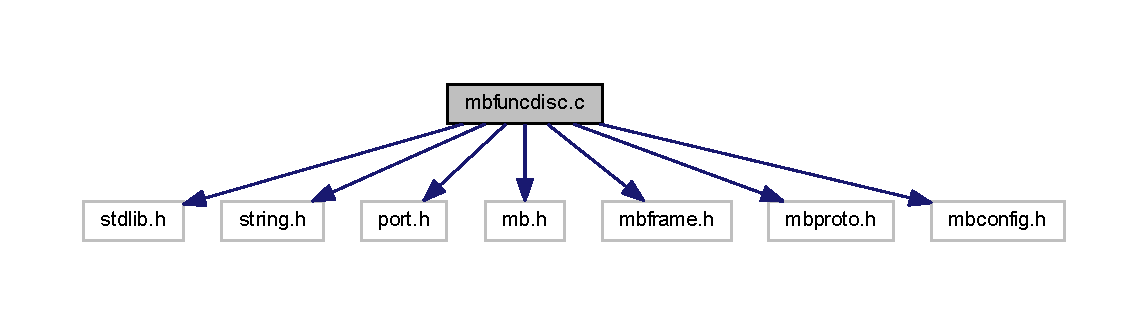
\includegraphics[width=350pt]{mbfuncdisc_8c__incl}
\end{center}
\end{figure}
\subsection*{Macros}
\begin{DoxyCompactItemize}
\item 
\#define {\bfseries M\+B\+\_\+\+P\+D\+U\+\_\+\+F\+U\+N\+C\+\_\+\+R\+E\+A\+D\+\_\+\+A\+D\+D\+R\+\_\+\+O\+FF}~( M\+B\+\_\+\+P\+D\+U\+\_\+\+D\+A\+T\+A\+\_\+\+O\+FF )\hypertarget{mbfuncdisc_8c_ab3c4b5bd48b2160671541e4026f2caae}{}\label{mbfuncdisc_8c_ab3c4b5bd48b2160671541e4026f2caae}

\item 
\#define {\bfseries M\+B\+\_\+\+P\+D\+U\+\_\+\+F\+U\+N\+C\+\_\+\+R\+E\+A\+D\+\_\+\+D\+I\+S\+C\+C\+N\+T\+\_\+\+O\+FF}~( M\+B\+\_\+\+P\+D\+U\+\_\+\+D\+A\+T\+A\+\_\+\+O\+FF + 2 )\hypertarget{mbfuncdisc_8c_a30dc5368359d0e3dcf168ba33ea65676}{}\label{mbfuncdisc_8c_a30dc5368359d0e3dcf168ba33ea65676}

\item 
\#define {\bfseries M\+B\+\_\+\+P\+D\+U\+\_\+\+F\+U\+N\+C\+\_\+\+R\+E\+A\+D\+\_\+\+S\+I\+ZE}~( 4 )\hypertarget{mbfuncdisc_8c_a968555f75801294753a5b2da91bea764}{}\label{mbfuncdisc_8c_a968555f75801294753a5b2da91bea764}

\item 
\#define {\bfseries M\+B\+\_\+\+P\+D\+U\+\_\+\+F\+U\+N\+C\+\_\+\+R\+E\+A\+D\+\_\+\+D\+I\+S\+C\+C\+N\+T\+\_\+\+M\+AX}~( 0x07\+D0 )\hypertarget{mbfuncdisc_8c_a01189d363bad2bce08666420491796ad}{}\label{mbfuncdisc_8c_a01189d363bad2bce08666420491796ad}

\end{DoxyCompactItemize}
\subsection*{Functions}
\begin{DoxyCompactItemize}
\item 
e\+M\+B\+Exception \hyperlink{mbfuncdisc_8c_ad5d2cc07a83fa7ea723ed734c905bc55}{prve\+M\+B\+Error2\+Exception} (e\+M\+B\+Error\+Code e\+Error\+Code)
\end{DoxyCompactItemize}


\subsection{Detailed Description}
Free\+R\+T\+OS Modbus Libary\+: A Modbus serial implementation for Free\+R\+T\+OS Copyright (C) 2006 Christian Walter \href{mailto:wolti@sil.at}{\tt wolti@sil.\+at}

This library is free software; you can redistribute it and/or modify it under the terms of the G\+NU Lesser General Public License as published by the Free Software Foundation; either version 2.\+1 of the License, or (at your option) any later version.

This library is distributed in the hope that it will be useful, but W\+I\+T\+H\+O\+UT A\+NY W\+A\+R\+R\+A\+N\+TY; without even the implied warranty of M\+E\+R\+C\+H\+A\+N\+T\+A\+B\+I\+L\+I\+TY or F\+I\+T\+N\+E\+SS F\+OR A P\+A\+R\+T\+I\+C\+U\+L\+AR P\+U\+R\+P\+O\+SE. See the G\+NU Lesser General Public License for more details.

You should have received a copy of the G\+NU Lesser General Public License along with this library; if not, write to the Free Software Foundation, Inc., 51 Franklin St, Fifth Floor, Boston, MA 02110-\/1301 U\+SA 

\subsection{Function Documentation}
\index{mbfuncdisc.\+c@{mbfuncdisc.\+c}!prve\+M\+B\+Error2\+Exception@{prve\+M\+B\+Error2\+Exception}}
\index{prve\+M\+B\+Error2\+Exception@{prve\+M\+B\+Error2\+Exception}!mbfuncdisc.\+c@{mbfuncdisc.\+c}}
\subsubsection[{\texorpdfstring{prve\+M\+B\+Error2\+Exception(e\+M\+B\+Error\+Code e\+Error\+Code)}{prveMBError2Exception(eMBErrorCode eErrorCode)}}]{\setlength{\rightskip}{0pt plus 5cm}e\+M\+B\+Exception prve\+M\+B\+Error2\+Exception (
\begin{DoxyParamCaption}
\item[{e\+M\+B\+Error\+Code}]{e\+Error\+Code}
\end{DoxyParamCaption}
)}\hypertarget{mbfuncdisc_8c_ad5d2cc07a83fa7ea723ed734c905bc55}{}\label{mbfuncdisc_8c_ad5d2cc07a83fa7ea723ed734c905bc55}


 \subsubsection*{prve\+M\+B\+Error2\+Exception }

Event Handler for G\+PI module \begin{DoxyVerb} @date                           DEC/02/2013
 @author                         FW_DEV_2
 @pre                            None
 @return                         None\end{DoxyVerb}
 

Definition at line 249 of file mbutils.\+c.


\hypertarget{mbfuncholding_8c}{}\section{mbfuncholding.\+c File Reference}
\label{mbfuncholding_8c}\index{mbfuncholding.\+c@{mbfuncholding.\+c}}
{\ttfamily \#include \char`\"{}stdlib.\+h\char`\"{}}\\*
{\ttfamily \#include \char`\"{}string.\+h\char`\"{}}\\*
{\ttfamily \#include \char`\"{}port.\+h\char`\"{}}\\*
{\ttfamily \#include \char`\"{}mb.\+h\char`\"{}}\\*
{\ttfamily \#include \char`\"{}mbframe.\+h\char`\"{}}\\*
{\ttfamily \#include \char`\"{}mbproto.\+h\char`\"{}}\\*
{\ttfamily \#include \char`\"{}mbconfig.\+h\char`\"{}}\\*
Include dependency graph for mbfuncholding.\+c\+:
\nopagebreak
\begin{figure}[H]
\begin{center}
\leavevmode
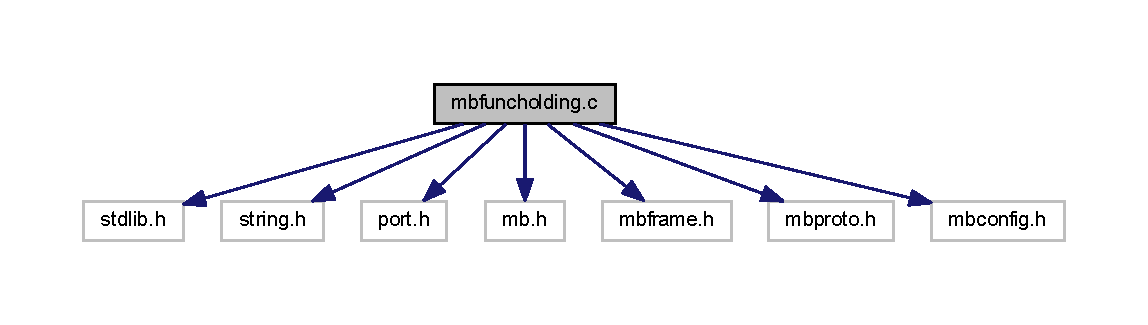
\includegraphics[width=350pt]{mbfuncholding_8c__incl}
\end{center}
\end{figure}
\subsection*{Macros}
\begin{DoxyCompactItemize}
\item 
\#define {\bfseries M\+B\+\_\+\+P\+D\+U\+\_\+\+F\+U\+N\+C\+\_\+\+R\+E\+A\+D\+\_\+\+A\+D\+D\+R\+\_\+\+O\+FF}~( M\+B\+\_\+\+P\+D\+U\+\_\+\+D\+A\+T\+A\+\_\+\+O\+FF + 0)\hypertarget{mbfuncholding_8c_ab3c4b5bd48b2160671541e4026f2caae}{}\label{mbfuncholding_8c_ab3c4b5bd48b2160671541e4026f2caae}

\item 
\#define {\bfseries M\+B\+\_\+\+P\+D\+U\+\_\+\+F\+U\+N\+C\+\_\+\+R\+E\+A\+D\+\_\+\+R\+E\+G\+C\+N\+T\+\_\+\+O\+FF}~( M\+B\+\_\+\+P\+D\+U\+\_\+\+D\+A\+T\+A\+\_\+\+O\+FF + 2 )\hypertarget{mbfuncholding_8c_ae5f5bb2d34c79141f425774b00ddd63b}{}\label{mbfuncholding_8c_ae5f5bb2d34c79141f425774b00ddd63b}

\item 
\#define {\bfseries M\+B\+\_\+\+P\+D\+U\+\_\+\+F\+U\+N\+C\+\_\+\+R\+E\+A\+D\+\_\+\+S\+I\+ZE}~( 4 )\hypertarget{mbfuncholding_8c_a968555f75801294753a5b2da91bea764}{}\label{mbfuncholding_8c_a968555f75801294753a5b2da91bea764}

\item 
\#define {\bfseries M\+B\+\_\+\+P\+D\+U\+\_\+\+F\+U\+N\+C\+\_\+\+R\+E\+A\+D\+\_\+\+R\+E\+G\+C\+N\+T\+\_\+\+M\+AX}~( 0x007\+D )\hypertarget{mbfuncholding_8c_ac66f1588a8138771b7ba2ec39319ae50}{}\label{mbfuncholding_8c_ac66f1588a8138771b7ba2ec39319ae50}

\item 
\#define {\bfseries M\+B\+\_\+\+P\+D\+U\+\_\+\+F\+U\+N\+C\+\_\+\+W\+R\+I\+T\+E\+\_\+\+A\+D\+D\+R\+\_\+\+O\+FF}~( M\+B\+\_\+\+P\+D\+U\+\_\+\+D\+A\+T\+A\+\_\+\+O\+FF + 0)\hypertarget{mbfuncholding_8c_a7e062d894a248db85a8270050f94e97e}{}\label{mbfuncholding_8c_a7e062d894a248db85a8270050f94e97e}

\item 
\#define {\bfseries M\+B\+\_\+\+P\+D\+U\+\_\+\+F\+U\+N\+C\+\_\+\+W\+R\+I\+T\+E\+\_\+\+V\+A\+L\+U\+E\+\_\+\+O\+FF}~( M\+B\+\_\+\+P\+D\+U\+\_\+\+D\+A\+T\+A\+\_\+\+O\+FF + 2 )\hypertarget{mbfuncholding_8c_a3366487f1f94813dbf7e118146fe0698}{}\label{mbfuncholding_8c_a3366487f1f94813dbf7e118146fe0698}

\item 
\#define {\bfseries M\+B\+\_\+\+P\+D\+U\+\_\+\+F\+U\+N\+C\+\_\+\+W\+R\+I\+T\+E\+\_\+\+S\+I\+ZE}~( 4 )\hypertarget{mbfuncholding_8c_a740439a1794d2f5be18109f38be50862}{}\label{mbfuncholding_8c_a740439a1794d2f5be18109f38be50862}

\item 
\#define {\bfseries M\+B\+\_\+\+P\+D\+U\+\_\+\+F\+U\+N\+C\+\_\+\+W\+R\+I\+T\+E\+\_\+\+M\+U\+L\+\_\+\+A\+D\+D\+R\+\_\+\+O\+FF}~( M\+B\+\_\+\+P\+D\+U\+\_\+\+D\+A\+T\+A\+\_\+\+O\+FF + 0 )\hypertarget{mbfuncholding_8c_ac28b968f1b4bbba124a7576e89a4ee96}{}\label{mbfuncholding_8c_ac28b968f1b4bbba124a7576e89a4ee96}

\item 
\#define {\bfseries M\+B\+\_\+\+P\+D\+U\+\_\+\+F\+U\+N\+C\+\_\+\+W\+R\+I\+T\+E\+\_\+\+M\+U\+L\+\_\+\+R\+E\+G\+C\+N\+T\+\_\+\+O\+FF}~( M\+B\+\_\+\+P\+D\+U\+\_\+\+D\+A\+T\+A\+\_\+\+O\+FF + 2 )\hypertarget{mbfuncholding_8c_afca29db54dc0ae16cdd93bb45ef7d4a3}{}\label{mbfuncholding_8c_afca29db54dc0ae16cdd93bb45ef7d4a3}

\item 
\#define {\bfseries M\+B\+\_\+\+P\+D\+U\+\_\+\+F\+U\+N\+C\+\_\+\+W\+R\+I\+T\+E\+\_\+\+M\+U\+L\+\_\+\+B\+Y\+T\+E\+C\+N\+T\+\_\+\+O\+FF}~( M\+B\+\_\+\+P\+D\+U\+\_\+\+D\+A\+T\+A\+\_\+\+O\+FF + 4 )\hypertarget{mbfuncholding_8c_ad40dd5916e0b4785402f5f583a288035}{}\label{mbfuncholding_8c_ad40dd5916e0b4785402f5f583a288035}

\item 
\#define {\bfseries M\+B\+\_\+\+P\+D\+U\+\_\+\+F\+U\+N\+C\+\_\+\+W\+R\+I\+T\+E\+\_\+\+M\+U\+L\+\_\+\+V\+A\+L\+U\+E\+S\+\_\+\+O\+FF}~( M\+B\+\_\+\+P\+D\+U\+\_\+\+D\+A\+T\+A\+\_\+\+O\+FF + 5 )\hypertarget{mbfuncholding_8c_a712155f8f2d0babedfa33f63a07e875b}{}\label{mbfuncholding_8c_a712155f8f2d0babedfa33f63a07e875b}

\item 
\#define {\bfseries M\+B\+\_\+\+P\+D\+U\+\_\+\+F\+U\+N\+C\+\_\+\+W\+R\+I\+T\+E\+\_\+\+M\+U\+L\+\_\+\+S\+I\+Z\+E\+\_\+\+M\+IN}~( 5 )\hypertarget{mbfuncholding_8c_a2e813e9e8d7743a9ae3f57bed67d0f64}{}\label{mbfuncholding_8c_a2e813e9e8d7743a9ae3f57bed67d0f64}

\item 
\#define {\bfseries M\+B\+\_\+\+P\+D\+U\+\_\+\+F\+U\+N\+C\+\_\+\+W\+R\+I\+T\+E\+\_\+\+M\+U\+L\+\_\+\+R\+E\+G\+C\+N\+T\+\_\+\+M\+AX}~( 0x0078 )\hypertarget{mbfuncholding_8c_a800fa95c7f048301acb5b8279693871f}{}\label{mbfuncholding_8c_a800fa95c7f048301acb5b8279693871f}

\item 
\#define {\bfseries M\+B\+\_\+\+P\+D\+U\+\_\+\+F\+U\+N\+C\+\_\+\+R\+E\+A\+D\+W\+R\+I\+T\+E\+\_\+\+R\+E\+A\+D\+\_\+\+A\+D\+D\+R\+\_\+\+O\+FF}~( M\+B\+\_\+\+P\+D\+U\+\_\+\+D\+A\+T\+A\+\_\+\+O\+FF + 0 )\hypertarget{mbfuncholding_8c_a73c8682fb51eaf5761a356af0361b4fb}{}\label{mbfuncholding_8c_a73c8682fb51eaf5761a356af0361b4fb}

\item 
\#define {\bfseries M\+B\+\_\+\+P\+D\+U\+\_\+\+F\+U\+N\+C\+\_\+\+R\+E\+A\+D\+W\+R\+I\+T\+E\+\_\+\+R\+E\+A\+D\+\_\+\+R\+E\+G\+C\+N\+T\+\_\+\+O\+FF}~( M\+B\+\_\+\+P\+D\+U\+\_\+\+D\+A\+T\+A\+\_\+\+O\+FF + 2 )\hypertarget{mbfuncholding_8c_aa52d7699dabfe567af4e0658772f36a0}{}\label{mbfuncholding_8c_aa52d7699dabfe567af4e0658772f36a0}

\item 
\#define {\bfseries M\+B\+\_\+\+P\+D\+U\+\_\+\+F\+U\+N\+C\+\_\+\+R\+E\+A\+D\+W\+R\+I\+T\+E\+\_\+\+W\+R\+I\+T\+E\+\_\+\+A\+D\+D\+R\+\_\+\+O\+FF}~( M\+B\+\_\+\+P\+D\+U\+\_\+\+D\+A\+T\+A\+\_\+\+O\+FF + 4 )\hypertarget{mbfuncholding_8c_a919f8364404198ac2ed92be74bec4655}{}\label{mbfuncholding_8c_a919f8364404198ac2ed92be74bec4655}

\item 
\#define {\bfseries M\+B\+\_\+\+P\+D\+U\+\_\+\+F\+U\+N\+C\+\_\+\+R\+E\+A\+D\+W\+R\+I\+T\+E\+\_\+\+W\+R\+I\+T\+E\+\_\+\+R\+E\+G\+C\+N\+T\+\_\+\+O\+FF}~( M\+B\+\_\+\+P\+D\+U\+\_\+\+D\+A\+T\+A\+\_\+\+O\+FF + 6 )\hypertarget{mbfuncholding_8c_a1551f9a31d4bb7a9d6942740ebbd0286}{}\label{mbfuncholding_8c_a1551f9a31d4bb7a9d6942740ebbd0286}

\item 
\#define {\bfseries M\+B\+\_\+\+P\+D\+U\+\_\+\+F\+U\+N\+C\+\_\+\+R\+E\+A\+D\+W\+R\+I\+T\+E\+\_\+\+B\+Y\+T\+E\+C\+N\+T\+\_\+\+O\+FF}~( M\+B\+\_\+\+P\+D\+U\+\_\+\+D\+A\+T\+A\+\_\+\+O\+FF + 8 )\hypertarget{mbfuncholding_8c_a0bb331fcae41846bf075898c9b7a93c6}{}\label{mbfuncholding_8c_a0bb331fcae41846bf075898c9b7a93c6}

\item 
\#define {\bfseries M\+B\+\_\+\+P\+D\+U\+\_\+\+F\+U\+N\+C\+\_\+\+R\+E\+A\+D\+W\+R\+I\+T\+E\+\_\+\+W\+R\+I\+T\+E\+\_\+\+V\+A\+L\+U\+E\+S\+\_\+\+O\+FF}~( M\+B\+\_\+\+P\+D\+U\+\_\+\+D\+A\+T\+A\+\_\+\+O\+FF + 9 )\hypertarget{mbfuncholding_8c_a491ef64901a1d102c45267a07dab2f1f}{}\label{mbfuncholding_8c_a491ef64901a1d102c45267a07dab2f1f}

\item 
\#define {\bfseries M\+B\+\_\+\+P\+D\+U\+\_\+\+F\+U\+N\+C\+\_\+\+R\+E\+A\+D\+W\+R\+I\+T\+E\+\_\+\+S\+I\+Z\+E\+\_\+\+M\+IN}~( 9 )\hypertarget{mbfuncholding_8c_a18562933be8dd65c5ac854fcb90af8b8}{}\label{mbfuncholding_8c_a18562933be8dd65c5ac854fcb90af8b8}

\end{DoxyCompactItemize}
\subsection*{Functions}
\begin{DoxyCompactItemize}
\item 
e\+M\+B\+Exception \hyperlink{mbfuncholding_8c_ad5d2cc07a83fa7ea723ed734c905bc55}{prve\+M\+B\+Error2\+Exception} (e\+M\+B\+Error\+Code e\+Error\+Code)
\end{DoxyCompactItemize}


\subsection{Detailed Description}
Free\+Modbus Libary\+: A portable Modbus implementation for Modbus A\+S\+C\+I\+I/\+R\+TU. Copyright (c) 2006 Christian Walter \href{mailto:wolti@sil.at}{\tt wolti@sil.\+at} All rights reserved.

Redistribution and use in source and binary forms, with or without modification, are permitted provided that the following conditions are met\+:
\begin{DoxyEnumerate}
\item Redistributions of source code must retain the above copyright notice, this list of conditions and the following disclaimer.
\item Redistributions in binary form must reproduce the above copyright notice, this list of conditions and the following disclaimer in the documentation and/or other materials provided with the distribution.
\item The name of the author may not be used to endorse or promote products derived from this software without specific prior written permission.
\end{DoxyEnumerate}

T\+H\+IS S\+O\+F\+T\+W\+A\+RE IS P\+R\+O\+V\+I\+D\+ED BY T\+HE A\+U\+T\+H\+OR ``\+AS IS\textquotesingle{}\textquotesingle{} A\+ND A\+NY E\+X\+P\+R\+E\+SS OR I\+M\+P\+L\+I\+ED W\+A\+R\+R\+A\+N\+T\+I\+ES, I\+N\+C\+L\+U\+D\+I\+NG, B\+UT N\+OT L\+I\+M\+I\+T\+ED TO, T\+HE I\+M\+P\+L\+I\+ED W\+A\+R\+R\+A\+N\+T\+I\+ES OF M\+E\+R\+C\+H\+A\+N\+T\+A\+B\+I\+L\+I\+TY A\+ND F\+I\+T\+N\+E\+SS F\+OR A P\+A\+R\+T\+I\+C\+U\+L\+AR P\+U\+R\+P\+O\+SE A\+RE D\+I\+S\+C\+L\+A\+I\+M\+ED. IN NO E\+V\+E\+NT S\+H\+A\+LL T\+HE A\+U\+T\+H\+OR BE L\+I\+A\+B\+LE F\+OR A\+NY D\+I\+R\+E\+CT, I\+N\+D\+I\+R\+E\+CT, I\+N\+C\+I\+D\+E\+N\+T\+AL, S\+P\+E\+C\+I\+AL, E\+X\+E\+M\+P\+L\+A\+RY, OR C\+O\+N\+S\+E\+Q\+U\+E\+N\+T\+I\+AL D\+A\+M\+A\+G\+ES (I\+N\+C\+L\+U\+D\+I\+NG, B\+UT N\+OT L\+I\+M\+I\+T\+ED TO, P\+R\+O\+C\+U\+R\+E\+M\+E\+NT OF S\+U\+B\+S\+T\+I\+T\+U\+TE G\+O\+O\+DS OR S\+E\+R\+V\+I\+C\+ES; L\+O\+SS OF U\+SE, D\+A\+TA, OR P\+R\+O\+F\+I\+TS; OR B\+U\+S\+I\+N\+E\+SS I\+N\+T\+E\+R\+R\+U\+P\+T\+I\+ON) H\+O\+W\+E\+V\+ER C\+A\+U\+S\+ED A\+ND ON A\+NY T\+H\+E\+O\+RY OF L\+I\+A\+B\+I\+L\+I\+TY, W\+H\+E\+T\+H\+ER IN C\+O\+N\+T\+R\+A\+CT, S\+T\+R\+I\+CT L\+I\+A\+B\+I\+L\+I\+TY, OR T\+O\+RT (I\+N\+C\+L\+U\+D\+I\+NG N\+E\+G\+L\+I\+G\+E\+N\+CE OR O\+T\+H\+E\+R\+W\+I\+SE) A\+R\+I\+S\+I\+NG IN A\+NY W\+AY O\+UT OF T\+HE U\+SE OF T\+H\+IS S\+O\+F\+T\+W\+A\+RE, E\+V\+EN IF A\+D\+V\+I\+S\+ED OF T\+HE P\+O\+S\+S\+I\+B\+I\+L\+I\+TY OF S\+U\+CH D\+A\+M\+A\+GE.

File\+: \begin{DoxyParagraph}{Id}
\hyperlink{mbfuncholding_8c}{mbfuncholding.\+c},v 1.\+12 2007/02/18 23\+:48\+:22 wolti Exp 
\end{DoxyParagraph}


\subsection{Function Documentation}
\index{mbfuncholding.\+c@{mbfuncholding.\+c}!prve\+M\+B\+Error2\+Exception@{prve\+M\+B\+Error2\+Exception}}
\index{prve\+M\+B\+Error2\+Exception@{prve\+M\+B\+Error2\+Exception}!mbfuncholding.\+c@{mbfuncholding.\+c}}
\subsubsection[{\texorpdfstring{prve\+M\+B\+Error2\+Exception(e\+M\+B\+Error\+Code e\+Error\+Code)}{prveMBError2Exception(eMBErrorCode eErrorCode)}}]{\setlength{\rightskip}{0pt plus 5cm}e\+M\+B\+Exception prve\+M\+B\+Error2\+Exception (
\begin{DoxyParamCaption}
\item[{e\+M\+B\+Error\+Code}]{e\+Error\+Code}
\end{DoxyParamCaption}
)}\hypertarget{mbfuncholding_8c_ad5d2cc07a83fa7ea723ed734c905bc55}{}\label{mbfuncholding_8c_ad5d2cc07a83fa7ea723ed734c905bc55}


 \subsubsection*{prve\+M\+B\+Error2\+Exception }

Event Handler for G\+PI module \begin{DoxyVerb} @date                           DEC/02/2013
 @author                         FW_DEV_2
 @pre                            None
 @return                         None\end{DoxyVerb}
 

Definition at line 249 of file mbutils.\+c.


\hypertarget{mbfuncinput_8c}{}\section{mbfuncinput.\+c File Reference}
\label{mbfuncinput_8c}\index{mbfuncinput.\+c@{mbfuncinput.\+c}}
{\ttfamily \#include \char`\"{}stdlib.\+h\char`\"{}}\\*
{\ttfamily \#include \char`\"{}string.\+h\char`\"{}}\\*
{\ttfamily \#include \char`\"{}port.\+h\char`\"{}}\\*
{\ttfamily \#include \char`\"{}mb.\+h\char`\"{}}\\*
{\ttfamily \#include \char`\"{}mbframe.\+h\char`\"{}}\\*
{\ttfamily \#include \char`\"{}mbproto.\+h\char`\"{}}\\*
{\ttfamily \#include \char`\"{}mbconfig.\+h\char`\"{}}\\*
Include dependency graph for mbfuncinput.\+c\+:
\nopagebreak
\begin{figure}[H]
\begin{center}
\leavevmode
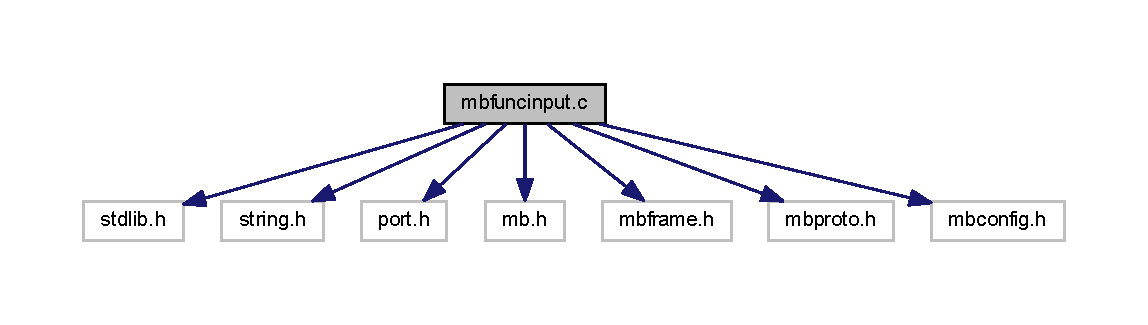
\includegraphics[width=350pt]{mbfuncinput_8c__incl}
\end{center}
\end{figure}
\subsection*{Macros}
\begin{DoxyCompactItemize}
\item 
\#define {\bfseries M\+B\+\_\+\+P\+D\+U\+\_\+\+F\+U\+N\+C\+\_\+\+R\+E\+A\+D\+\_\+\+A\+D\+D\+R\+\_\+\+O\+FF}~( M\+B\+\_\+\+P\+D\+U\+\_\+\+D\+A\+T\+A\+\_\+\+O\+FF )\hypertarget{mbfuncinput_8c_ab3c4b5bd48b2160671541e4026f2caae}{}\label{mbfuncinput_8c_ab3c4b5bd48b2160671541e4026f2caae}

\item 
\#define {\bfseries M\+B\+\_\+\+P\+D\+U\+\_\+\+F\+U\+N\+C\+\_\+\+R\+E\+A\+D\+\_\+\+R\+E\+G\+C\+N\+T\+\_\+\+O\+FF}~( M\+B\+\_\+\+P\+D\+U\+\_\+\+D\+A\+T\+A\+\_\+\+O\+FF + 2 )\hypertarget{mbfuncinput_8c_ae5f5bb2d34c79141f425774b00ddd63b}{}\label{mbfuncinput_8c_ae5f5bb2d34c79141f425774b00ddd63b}

\item 
\#define {\bfseries M\+B\+\_\+\+P\+D\+U\+\_\+\+F\+U\+N\+C\+\_\+\+R\+E\+A\+D\+\_\+\+S\+I\+ZE}~( 4 )\hypertarget{mbfuncinput_8c_a968555f75801294753a5b2da91bea764}{}\label{mbfuncinput_8c_a968555f75801294753a5b2da91bea764}

\item 
\#define {\bfseries M\+B\+\_\+\+P\+D\+U\+\_\+\+F\+U\+N\+C\+\_\+\+R\+E\+A\+D\+\_\+\+R\+E\+G\+C\+N\+T\+\_\+\+M\+AX}~( 0x007\+D )\hypertarget{mbfuncinput_8c_ac66f1588a8138771b7ba2ec39319ae50}{}\label{mbfuncinput_8c_ac66f1588a8138771b7ba2ec39319ae50}

\item 
\#define {\bfseries M\+B\+\_\+\+P\+D\+U\+\_\+\+F\+U\+N\+C\+\_\+\+R\+E\+A\+D\+\_\+\+R\+S\+P\+\_\+\+B\+Y\+T\+E\+C\+N\+T\+\_\+\+O\+FF}~( M\+B\+\_\+\+P\+D\+U\+\_\+\+D\+A\+T\+A\+\_\+\+O\+FF )\hypertarget{mbfuncinput_8c_aed5d97217f5de85de9931062e875302a}{}\label{mbfuncinput_8c_aed5d97217f5de85de9931062e875302a}

\end{DoxyCompactItemize}
\subsection*{Functions}
\begin{DoxyCompactItemize}
\item 
e\+M\+B\+Exception \hyperlink{mbfuncinput_8c_ad5d2cc07a83fa7ea723ed734c905bc55}{prve\+M\+B\+Error2\+Exception} (e\+M\+B\+Error\+Code e\+Error\+Code)
\end{DoxyCompactItemize}


\subsection{Detailed Description}
Free\+Modbus Libary\+: A portable Modbus implementation for Modbus A\+S\+C\+I\+I/\+R\+TU. Copyright (c) 2006 Christian Walter \href{mailto:wolti@sil.at}{\tt wolti@sil.\+at} All rights reserved.

Redistribution and use in source and binary forms, with or without modification, are permitted provided that the following conditions are met\+:
\begin{DoxyEnumerate}
\item Redistributions of source code must retain the above copyright notice, this list of conditions and the following disclaimer.
\item Redistributions in binary form must reproduce the above copyright notice, this list of conditions and the following disclaimer in the documentation and/or other materials provided with the distribution.
\item The name of the author may not be used to endorse or promote products derived from this software without specific prior written permission.
\end{DoxyEnumerate}

T\+H\+IS S\+O\+F\+T\+W\+A\+RE IS P\+R\+O\+V\+I\+D\+ED BY T\+HE A\+U\+T\+H\+OR ``\+AS IS\textquotesingle{}\textquotesingle{} A\+ND A\+NY E\+X\+P\+R\+E\+SS OR I\+M\+P\+L\+I\+ED W\+A\+R\+R\+A\+N\+T\+I\+ES, I\+N\+C\+L\+U\+D\+I\+NG, B\+UT N\+OT L\+I\+M\+I\+T\+ED TO, T\+HE I\+M\+P\+L\+I\+ED W\+A\+R\+R\+A\+N\+T\+I\+ES OF M\+E\+R\+C\+H\+A\+N\+T\+A\+B\+I\+L\+I\+TY A\+ND F\+I\+T\+N\+E\+SS F\+OR A P\+A\+R\+T\+I\+C\+U\+L\+AR P\+U\+R\+P\+O\+SE A\+RE D\+I\+S\+C\+L\+A\+I\+M\+ED. IN NO E\+V\+E\+NT S\+H\+A\+LL T\+HE A\+U\+T\+H\+OR BE L\+I\+A\+B\+LE F\+OR A\+NY D\+I\+R\+E\+CT, I\+N\+D\+I\+R\+E\+CT, I\+N\+C\+I\+D\+E\+N\+T\+AL, S\+P\+E\+C\+I\+AL, E\+X\+E\+M\+P\+L\+A\+RY, OR C\+O\+N\+S\+E\+Q\+U\+E\+N\+T\+I\+AL D\+A\+M\+A\+G\+ES (I\+N\+C\+L\+U\+D\+I\+NG, B\+UT N\+OT L\+I\+M\+I\+T\+ED TO, P\+R\+O\+C\+U\+R\+E\+M\+E\+NT OF S\+U\+B\+S\+T\+I\+T\+U\+TE G\+O\+O\+DS OR S\+E\+R\+V\+I\+C\+ES; L\+O\+SS OF U\+SE, D\+A\+TA, OR P\+R\+O\+F\+I\+TS; OR B\+U\+S\+I\+N\+E\+SS I\+N\+T\+E\+R\+R\+U\+P\+T\+I\+ON) H\+O\+W\+E\+V\+ER C\+A\+U\+S\+ED A\+ND ON A\+NY T\+H\+E\+O\+RY OF L\+I\+A\+B\+I\+L\+I\+TY, W\+H\+E\+T\+H\+ER IN C\+O\+N\+T\+R\+A\+CT, S\+T\+R\+I\+CT L\+I\+A\+B\+I\+L\+I\+TY, OR T\+O\+RT (I\+N\+C\+L\+U\+D\+I\+NG N\+E\+G\+L\+I\+G\+E\+N\+CE OR O\+T\+H\+E\+R\+W\+I\+SE) A\+R\+I\+S\+I\+NG IN A\+NY W\+AY O\+UT OF T\+HE U\+SE OF T\+H\+IS S\+O\+F\+T\+W\+A\+RE, E\+V\+EN IF A\+D\+V\+I\+S\+ED OF T\+HE P\+O\+S\+S\+I\+B\+I\+L\+I\+TY OF S\+U\+CH D\+A\+M\+A\+GE.

File\+: \begin{DoxyParagraph}{Id}
\hyperlink{mbfuncinput_8c}{mbfuncinput.\+c},v 1.\+10 2007/09/12 10\+:15\+:56 wolti Exp 
\end{DoxyParagraph}


\subsection{Function Documentation}
\index{mbfuncinput.\+c@{mbfuncinput.\+c}!prve\+M\+B\+Error2\+Exception@{prve\+M\+B\+Error2\+Exception}}
\index{prve\+M\+B\+Error2\+Exception@{prve\+M\+B\+Error2\+Exception}!mbfuncinput.\+c@{mbfuncinput.\+c}}
\subsubsection[{\texorpdfstring{prve\+M\+B\+Error2\+Exception(e\+M\+B\+Error\+Code e\+Error\+Code)}{prveMBError2Exception(eMBErrorCode eErrorCode)}}]{\setlength{\rightskip}{0pt plus 5cm}e\+M\+B\+Exception prve\+M\+B\+Error2\+Exception (
\begin{DoxyParamCaption}
\item[{e\+M\+B\+Error\+Code}]{e\+Error\+Code}
\end{DoxyParamCaption}
)}\hypertarget{mbfuncinput_8c_ad5d2cc07a83fa7ea723ed734c905bc55}{}\label{mbfuncinput_8c_ad5d2cc07a83fa7ea723ed734c905bc55}


 \subsubsection*{prve\+M\+B\+Error2\+Exception }

Event Handler for G\+PI module \begin{DoxyVerb} @date                           DEC/02/2013
 @author                         FW_DEV_2
 @pre                            None
 @return                         None\end{DoxyVerb}
 

Definition at line 249 of file mbutils.\+c.


\hypertarget{mbfuncother_8c}{}\section{mbfuncother.\+c File Reference}
\label{mbfuncother_8c}\index{mbfuncother.\+c@{mbfuncother.\+c}}
{\ttfamily \#include \char`\"{}stdlib.\+h\char`\"{}}\\*
{\ttfamily \#include \char`\"{}string.\+h\char`\"{}}\\*
{\ttfamily \#include \char`\"{}port.\+h\char`\"{}}\\*
{\ttfamily \#include \char`\"{}mb.\+h\char`\"{}}\\*
{\ttfamily \#include \char`\"{}mbframe.\+h\char`\"{}}\\*
{\ttfamily \#include \char`\"{}mbproto.\+h\char`\"{}}\\*
{\ttfamily \#include \char`\"{}mbconfig.\+h\char`\"{}}\\*
Include dependency graph for mbfuncother.\+c\+:
\nopagebreak
\begin{figure}[H]
\begin{center}
\leavevmode
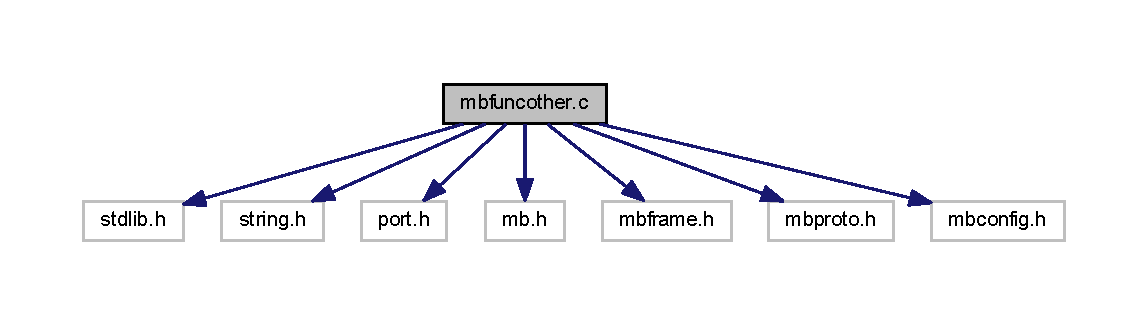
\includegraphics[width=350pt]{mbfuncother_8c__incl}
\end{center}
\end{figure}


\subsection{Detailed Description}
Free\+Modbus Libary\+: A portable Modbus implementation for Modbus A\+S\+C\+I\+I/\+R\+TU. Copyright (c) 2006 Christian Walter \href{mailto:wolti@sil.at}{\tt wolti@sil.\+at} All rights reserved.

Redistribution and use in source and binary forms, with or without modification, are permitted provided that the following conditions are met\+:
\begin{DoxyEnumerate}
\item Redistributions of source code must retain the above copyright notice, this list of conditions and the following disclaimer.
\item Redistributions in binary form must reproduce the above copyright notice, this list of conditions and the following disclaimer in the documentation and/or other materials provided with the distribution.
\item The name of the author may not be used to endorse or promote products derived from this software without specific prior written permission.
\end{DoxyEnumerate}

T\+H\+IS S\+O\+F\+T\+W\+A\+RE IS P\+R\+O\+V\+I\+D\+ED BY T\+HE A\+U\+T\+H\+OR ``\+AS IS\textquotesingle{}\textquotesingle{} A\+ND A\+NY E\+X\+P\+R\+E\+SS OR I\+M\+P\+L\+I\+ED W\+A\+R\+R\+A\+N\+T\+I\+ES, I\+N\+C\+L\+U\+D\+I\+NG, B\+UT N\+OT L\+I\+M\+I\+T\+ED TO, T\+HE I\+M\+P\+L\+I\+ED W\+A\+R\+R\+A\+N\+T\+I\+ES OF M\+E\+R\+C\+H\+A\+N\+T\+A\+B\+I\+L\+I\+TY A\+ND F\+I\+T\+N\+E\+SS F\+OR A P\+A\+R\+T\+I\+C\+U\+L\+AR P\+U\+R\+P\+O\+SE A\+RE D\+I\+S\+C\+L\+A\+I\+M\+ED. IN NO E\+V\+E\+NT S\+H\+A\+LL T\+HE A\+U\+T\+H\+OR BE L\+I\+A\+B\+LE F\+OR A\+NY D\+I\+R\+E\+CT, I\+N\+D\+I\+R\+E\+CT, I\+N\+C\+I\+D\+E\+N\+T\+AL, S\+P\+E\+C\+I\+AL, E\+X\+E\+M\+P\+L\+A\+RY, OR C\+O\+N\+S\+E\+Q\+U\+E\+N\+T\+I\+AL D\+A\+M\+A\+G\+ES (I\+N\+C\+L\+U\+D\+I\+NG, B\+UT N\+OT L\+I\+M\+I\+T\+ED TO, P\+R\+O\+C\+U\+R\+E\+M\+E\+NT OF S\+U\+B\+S\+T\+I\+T\+U\+TE G\+O\+O\+DS OR S\+E\+R\+V\+I\+C\+ES; L\+O\+SS OF U\+SE, D\+A\+TA, OR P\+R\+O\+F\+I\+TS; OR B\+U\+S\+I\+N\+E\+SS I\+N\+T\+E\+R\+R\+U\+P\+T\+I\+ON) H\+O\+W\+E\+V\+ER C\+A\+U\+S\+ED A\+ND ON A\+NY T\+H\+E\+O\+RY OF L\+I\+A\+B\+I\+L\+I\+TY, W\+H\+E\+T\+H\+ER IN C\+O\+N\+T\+R\+A\+CT, S\+T\+R\+I\+CT L\+I\+A\+B\+I\+L\+I\+TY, OR T\+O\+RT (I\+N\+C\+L\+U\+D\+I\+NG N\+E\+G\+L\+I\+G\+E\+N\+CE OR O\+T\+H\+E\+R\+W\+I\+SE) A\+R\+I\+S\+I\+NG IN A\+NY W\+AY O\+UT OF T\+HE U\+SE OF T\+H\+IS S\+O\+F\+T\+W\+A\+RE, E\+V\+EN IF A\+D\+V\+I\+S\+ED OF T\+HE P\+O\+S\+S\+I\+B\+I\+L\+I\+TY OF S\+U\+CH D\+A\+M\+A\+GE.

File\+: \begin{DoxyParagraph}{Id}
\hyperlink{mbfuncother_8c}{mbfuncother.\+c},v 1.\+8 2006/12/07 22\+:10\+:34 wolti Exp 
\end{DoxyParagraph}

\hypertarget{mbrtu_8c}{}\section{mbrtu.\+c File Reference}
\label{mbrtu_8c}\index{mbrtu.\+c@{mbrtu.\+c}}
{\ttfamily \#include \char`\"{}stdlib.\+h\char`\"{}}\\*
{\ttfamily \#include \char`\"{}string.\+h\char`\"{}}\\*
{\ttfamily \#include \char`\"{}port.\+h\char`\"{}}\\*
{\ttfamily \#include \char`\"{}mb.\+h\char`\"{}}\\*
{\ttfamily \#include \char`\"{}mbrtu.\+h\char`\"{}}\\*
{\ttfamily \#include \char`\"{}mbframe.\+h\char`\"{}}\\*
{\ttfamily \#include \char`\"{}mbcrc.\+h\char`\"{}}\\*
{\ttfamily \#include \char`\"{}mbport.\+h\char`\"{}}\\*
Include dependency graph for mbrtu.\+c\+:
\nopagebreak
\begin{figure}[H]
\begin{center}
\leavevmode
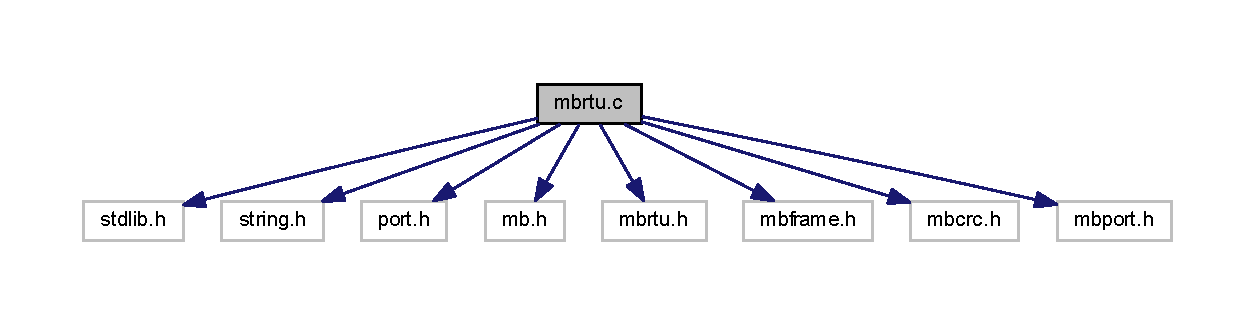
\includegraphics[width=350pt]{mbrtu_8c__incl}
\end{center}
\end{figure}
\subsection*{Macros}
\begin{DoxyCompactItemize}
\item 
\#define \hyperlink{mbrtu_8c_ae0dc27c9b034c5177638e9eef79d48a7}{M\+B\+\_\+\+S\+E\+R\+\_\+\+P\+D\+U\+\_\+\+S\+I\+Z\+E\+\_\+\+M\+IN}~4
\item 
\#define \hyperlink{mbrtu_8c_ad7e9cfdbd55413153a9a862d824a149f}{M\+B\+\_\+\+S\+E\+R\+\_\+\+P\+D\+U\+\_\+\+S\+I\+Z\+E\+\_\+\+M\+AX}~256
\item 
\#define \hyperlink{mbrtu_8c_afc5bf40f988e11036cdd8a44c1402d52}{M\+B\+\_\+\+S\+E\+R\+\_\+\+P\+D\+U\+\_\+\+S\+I\+Z\+E\+\_\+\+C\+RC}~2
\item 
\#define \hyperlink{mbrtu_8c_afd3d56d60a90ce4cb9858d305f446630}{M\+B\+\_\+\+S\+E\+R\+\_\+\+P\+D\+U\+\_\+\+A\+D\+D\+R\+\_\+\+O\+FF}~0
\item 
\#define \hyperlink{mbrtu_8c_ab20d539d6366275b4f75f181908ca207}{M\+B\+\_\+\+S\+E\+R\+\_\+\+P\+D\+U\+\_\+\+P\+D\+U\+\_\+\+O\+FF}~1
\end{DoxyCompactItemize}
\subsection*{Enumerations}
\begin{DoxyCompactItemize}
\item 
enum \hyperlink{mbrtu_8c_ada71af7b20c01523339e4f2ff95feefb}{e\+M\+B\+Rcv\+State} \{ \\*
\hyperlink{mbrtu_8c_ada71af7b20c01523339e4f2ff95feefba2b2395354f5e0566929bd52408265fb3}{S\+T\+A\+T\+E\+\_\+\+R\+X\+\_\+\+I\+N\+IT}, 
\\*
\hyperlink{mbrtu_8c_ada71af7b20c01523339e4f2ff95feefba516714125b01eae93e5cb693fdc3a9e0}{S\+T\+A\+T\+E\+\_\+\+R\+X\+\_\+\+I\+D\+LE}, 
\\*
\hyperlink{mbrtu_8c_ada71af7b20c01523339e4f2ff95feefba6489a66156527784ec30b45fc5ffe43b}{S\+T\+A\+T\+E\+\_\+\+R\+X\+\_\+\+R\+CV}, 
\\*
\hyperlink{mbrtu_8c_ada71af7b20c01523339e4f2ff95feefbafbb71fcd5e10dfbcc33a8f5a00df1f95}{S\+T\+A\+T\+E\+\_\+\+R\+X\+\_\+\+E\+R\+R\+OR}
 \}
\item 
enum \hyperlink{mbrtu_8c_ac877d5e834a5d5b2f80240c0a90d7fef}{e\+M\+B\+Snd\+State} \{ \\*
\hyperlink{mbrtu_8c_ac877d5e834a5d5b2f80240c0a90d7fefab1bd9fcf7cdb346f72d012adfca4767a}{S\+T\+A\+T\+E\+\_\+\+T\+X\+\_\+\+I\+D\+LE}, 
\\*
\hyperlink{mbrtu_8c_ac877d5e834a5d5b2f80240c0a90d7fefa99b8ef6f95d0035f9519dcb2889b3a83}{S\+T\+A\+T\+E\+\_\+\+T\+X\+\_\+\+X\+M\+IT}
 \}
\end{DoxyCompactItemize}
\subsection*{Functions}
\begin{DoxyCompactItemize}
\item 
e\+M\+B\+Error\+Code \hyperlink{mbrtu_8c_a52738b46d7f3be581582d30cfb2bfcb8}{e\+M\+B\+R\+T\+U\+Init} (U\+C\+H\+AR uc\+Slave\+Address, U\+C\+H\+AR uc\+Port, U\+L\+O\+NG ul\+Baud\+Rate, e\+M\+B\+Parity e\+Parity)
\item 
void \hyperlink{mbrtu_8c_ae342bae030ea291a6e8a2fe3d2d0abeb}{e\+M\+B\+R\+T\+U\+Start} (void)
\item 
void \hyperlink{mbrtu_8c_a3d44ef4747b7202d37142ef1aaea493b}{e\+M\+B\+R\+T\+U\+Stop} (void)
\item 
e\+M\+B\+Error\+Code \hyperlink{mbrtu_8c_a669fd79aadbd1cc49ac4f11382dc15d9}{e\+M\+B\+R\+T\+U\+Receive} (U\+C\+H\+AR $\ast$puc\+Rcv\+Address, U\+C\+H\+AR $\ast$$\ast$puc\+Frame, U\+S\+H\+O\+RT $\ast$pus\+Length)
\item 
e\+M\+B\+Error\+Code \hyperlink{mbrtu_8c_a6feb0c70f52d3ef74da1cfbdc10d1ab0}{e\+M\+B\+R\+T\+U\+Send} (U\+C\+H\+AR uc\+Slave\+Address, const U\+C\+H\+AR $\ast$puc\+Frame, U\+S\+H\+O\+RT us\+Length)
\item 
B\+O\+OL \hyperlink{mbrtu_8c_a447f45f582daab2600cad612b00120b0}{x\+M\+B\+R\+T\+U\+Receive\+F\+SM} (void)
\item 
B\+O\+OL \hyperlink{mbrtu_8c_a663e5daf0be0f2426a72c531c91d423f}{x\+M\+B\+R\+T\+U\+Transmit\+F\+SM} (void)
\item 
B\+O\+OL \hyperlink{mbrtu_8c_ac6302a8b67c6b82ae49e6c9d6a9795da}{x\+M\+B\+R\+T\+U\+Timer\+T35\+Expired} (void)
\end{DoxyCompactItemize}
\subsection*{Variables}
\begin{DoxyCompactItemize}
\item 
volatile U\+C\+H\+AR {\bfseries uc\+R\+T\+U\+Buf} \mbox{[}\hyperlink{mbrtu_8c_ad7e9cfdbd55413153a9a862d824a149f}{M\+B\+\_\+\+S\+E\+R\+\_\+\+P\+D\+U\+\_\+\+S\+I\+Z\+E\+\_\+\+M\+AX}\mbox{]}\hypertarget{mbrtu_8c_a0fa63f7bfbfea7ac20cce55d94cf3d53}{}\label{mbrtu_8c_a0fa63f7bfbfea7ac20cce55d94cf3d53}

\end{DoxyCompactItemize}


\subsection{Detailed Description}
Free\+Modbus Libary\+: A portable Modbus implementation for Modbus A\+S\+C\+I\+I/\+R\+TU. Copyright (c) 2006 Christian Walter \href{mailto:wolti@sil.at}{\tt wolti@sil.\+at} All rights reserved.

Redistribution and use in source and binary forms, with or without modification, are permitted provided that the following conditions are met\+:
\begin{DoxyEnumerate}
\item Redistributions of source code must retain the above copyright notice, this list of conditions and the following disclaimer.
\item Redistributions in binary form must reproduce the above copyright notice, this list of conditions and the following disclaimer in the documentation and/or other materials provided with the distribution.
\item The name of the author may not be used to endorse or promote products derived from this software without specific prior written permission.
\end{DoxyEnumerate}

T\+H\+IS S\+O\+F\+T\+W\+A\+RE IS P\+R\+O\+V\+I\+D\+ED BY T\+HE A\+U\+T\+H\+OR ``\+AS IS\textquotesingle{}\textquotesingle{} A\+ND A\+NY E\+X\+P\+R\+E\+SS OR I\+M\+P\+L\+I\+ED W\+A\+R\+R\+A\+N\+T\+I\+ES, I\+N\+C\+L\+U\+D\+I\+NG, B\+UT N\+OT L\+I\+M\+I\+T\+ED TO, T\+HE I\+M\+P\+L\+I\+ED W\+A\+R\+R\+A\+N\+T\+I\+ES OF M\+E\+R\+C\+H\+A\+N\+T\+A\+B\+I\+L\+I\+TY A\+ND F\+I\+T\+N\+E\+SS F\+OR A P\+A\+R\+T\+I\+C\+U\+L\+AR P\+U\+R\+P\+O\+SE A\+RE D\+I\+S\+C\+L\+A\+I\+M\+ED. IN NO E\+V\+E\+NT S\+H\+A\+LL T\+HE A\+U\+T\+H\+OR BE L\+I\+A\+B\+LE F\+OR A\+NY D\+I\+R\+E\+CT, I\+N\+D\+I\+R\+E\+CT, I\+N\+C\+I\+D\+E\+N\+T\+AL, S\+P\+E\+C\+I\+AL, E\+X\+E\+M\+P\+L\+A\+RY, OR C\+O\+N\+S\+E\+Q\+U\+E\+N\+T\+I\+AL D\+A\+M\+A\+G\+ES (I\+N\+C\+L\+U\+D\+I\+NG, B\+UT N\+OT L\+I\+M\+I\+T\+ED TO, P\+R\+O\+C\+U\+R\+E\+M\+E\+NT OF S\+U\+B\+S\+T\+I\+T\+U\+TE G\+O\+O\+DS OR S\+E\+R\+V\+I\+C\+ES; L\+O\+SS OF U\+SE, D\+A\+TA, OR P\+R\+O\+F\+I\+TS; OR B\+U\+S\+I\+N\+E\+SS I\+N\+T\+E\+R\+R\+U\+P\+T\+I\+ON) H\+O\+W\+E\+V\+ER C\+A\+U\+S\+ED A\+ND ON A\+NY T\+H\+E\+O\+RY OF L\+I\+A\+B\+I\+L\+I\+TY, W\+H\+E\+T\+H\+ER IN C\+O\+N\+T\+R\+A\+CT, S\+T\+R\+I\+CT L\+I\+A\+B\+I\+L\+I\+TY, OR T\+O\+RT (I\+N\+C\+L\+U\+D\+I\+NG N\+E\+G\+L\+I\+G\+E\+N\+CE OR O\+T\+H\+E\+R\+W\+I\+SE) A\+R\+I\+S\+I\+NG IN A\+NY W\+AY O\+UT OF T\+HE U\+SE OF T\+H\+IS S\+O\+F\+T\+W\+A\+RE, E\+V\+EN IF A\+D\+V\+I\+S\+ED OF T\+HE P\+O\+S\+S\+I\+B\+I\+L\+I\+TY OF S\+U\+CH D\+A\+M\+A\+GE.

File\+: \begin{DoxyParagraph}{Id}
\hyperlink{mbrtu_8c}{mbrtu.\+c},v 1.\+18 2007/09/12 10\+:15\+:56 wolti Exp 
\end{DoxyParagraph}


\subsection{Macro Definition Documentation}
\index{mbrtu.\+c@{mbrtu.\+c}!M\+B\+\_\+\+S\+E\+R\+\_\+\+P\+D\+U\+\_\+\+S\+I\+Z\+E\+\_\+\+M\+IN@{M\+B\+\_\+\+S\+E\+R\+\_\+\+P\+D\+U\+\_\+\+S\+I\+Z\+E\+\_\+\+M\+IN}}
\index{M\+B\+\_\+\+S\+E\+R\+\_\+\+P\+D\+U\+\_\+\+S\+I\+Z\+E\+\_\+\+M\+IN@{M\+B\+\_\+\+S\+E\+R\+\_\+\+P\+D\+U\+\_\+\+S\+I\+Z\+E\+\_\+\+M\+IN}!mbrtu.\+c@{mbrtu.\+c}}
\subsubsection[{\texorpdfstring{M\+B\+\_\+\+S\+E\+R\+\_\+\+P\+D\+U\+\_\+\+S\+I\+Z\+E\+\_\+\+M\+IN}{MB_SER_PDU_SIZE_MIN}}]{\setlength{\rightskip}{0pt plus 5cm}\#define M\+B\+\_\+\+S\+E\+R\+\_\+\+P\+D\+U\+\_\+\+S\+I\+Z\+E\+\_\+\+M\+IN~4}\hypertarget{mbrtu_8c_ae0dc27c9b034c5177638e9eef79d48a7}{}\label{mbrtu_8c_ae0dc27c9b034c5177638e9eef79d48a7}
Minimum size of a Modbus R\+TU frame. 

Definition at line 49 of file mbrtu.\+c.

\index{mbrtu.\+c@{mbrtu.\+c}!M\+B\+\_\+\+S\+E\+R\+\_\+\+P\+D\+U\+\_\+\+S\+I\+Z\+E\+\_\+\+M\+AX@{M\+B\+\_\+\+S\+E\+R\+\_\+\+P\+D\+U\+\_\+\+S\+I\+Z\+E\+\_\+\+M\+AX}}
\index{M\+B\+\_\+\+S\+E\+R\+\_\+\+P\+D\+U\+\_\+\+S\+I\+Z\+E\+\_\+\+M\+AX@{M\+B\+\_\+\+S\+E\+R\+\_\+\+P\+D\+U\+\_\+\+S\+I\+Z\+E\+\_\+\+M\+AX}!mbrtu.\+c@{mbrtu.\+c}}
\subsubsection[{\texorpdfstring{M\+B\+\_\+\+S\+E\+R\+\_\+\+P\+D\+U\+\_\+\+S\+I\+Z\+E\+\_\+\+M\+AX}{MB_SER_PDU_SIZE_MAX}}]{\setlength{\rightskip}{0pt plus 5cm}\#define M\+B\+\_\+\+S\+E\+R\+\_\+\+P\+D\+U\+\_\+\+S\+I\+Z\+E\+\_\+\+M\+AX~256}\hypertarget{mbrtu_8c_ad7e9cfdbd55413153a9a862d824a149f}{}\label{mbrtu_8c_ad7e9cfdbd55413153a9a862d824a149f}
Maximum size of a Modbus R\+TU frame. 

Definition at line 50 of file mbrtu.\+c.

\index{mbrtu.\+c@{mbrtu.\+c}!M\+B\+\_\+\+S\+E\+R\+\_\+\+P\+D\+U\+\_\+\+S\+I\+Z\+E\+\_\+\+C\+RC@{M\+B\+\_\+\+S\+E\+R\+\_\+\+P\+D\+U\+\_\+\+S\+I\+Z\+E\+\_\+\+C\+RC}}
\index{M\+B\+\_\+\+S\+E\+R\+\_\+\+P\+D\+U\+\_\+\+S\+I\+Z\+E\+\_\+\+C\+RC@{M\+B\+\_\+\+S\+E\+R\+\_\+\+P\+D\+U\+\_\+\+S\+I\+Z\+E\+\_\+\+C\+RC}!mbrtu.\+c@{mbrtu.\+c}}
\subsubsection[{\texorpdfstring{M\+B\+\_\+\+S\+E\+R\+\_\+\+P\+D\+U\+\_\+\+S\+I\+Z\+E\+\_\+\+C\+RC}{MB_SER_PDU_SIZE_CRC}}]{\setlength{\rightskip}{0pt plus 5cm}\#define M\+B\+\_\+\+S\+E\+R\+\_\+\+P\+D\+U\+\_\+\+S\+I\+Z\+E\+\_\+\+C\+RC~2}\hypertarget{mbrtu_8c_afc5bf40f988e11036cdd8a44c1402d52}{}\label{mbrtu_8c_afc5bf40f988e11036cdd8a44c1402d52}
Size of C\+RC field in P\+DU. 

Definition at line 51 of file mbrtu.\+c.

\index{mbrtu.\+c@{mbrtu.\+c}!M\+B\+\_\+\+S\+E\+R\+\_\+\+P\+D\+U\+\_\+\+A\+D\+D\+R\+\_\+\+O\+FF@{M\+B\+\_\+\+S\+E\+R\+\_\+\+P\+D\+U\+\_\+\+A\+D\+D\+R\+\_\+\+O\+FF}}
\index{M\+B\+\_\+\+S\+E\+R\+\_\+\+P\+D\+U\+\_\+\+A\+D\+D\+R\+\_\+\+O\+FF@{M\+B\+\_\+\+S\+E\+R\+\_\+\+P\+D\+U\+\_\+\+A\+D\+D\+R\+\_\+\+O\+FF}!mbrtu.\+c@{mbrtu.\+c}}
\subsubsection[{\texorpdfstring{M\+B\+\_\+\+S\+E\+R\+\_\+\+P\+D\+U\+\_\+\+A\+D\+D\+R\+\_\+\+O\+FF}{MB_SER_PDU_ADDR_OFF}}]{\setlength{\rightskip}{0pt plus 5cm}\#define M\+B\+\_\+\+S\+E\+R\+\_\+\+P\+D\+U\+\_\+\+A\+D\+D\+R\+\_\+\+O\+FF~0}\hypertarget{mbrtu_8c_afd3d56d60a90ce4cb9858d305f446630}{}\label{mbrtu_8c_afd3d56d60a90ce4cb9858d305f446630}
Offset of slave address in Ser-\/\+P\+DU. 

Definition at line 52 of file mbrtu.\+c.

\index{mbrtu.\+c@{mbrtu.\+c}!M\+B\+\_\+\+S\+E\+R\+\_\+\+P\+D\+U\+\_\+\+P\+D\+U\+\_\+\+O\+FF@{M\+B\+\_\+\+S\+E\+R\+\_\+\+P\+D\+U\+\_\+\+P\+D\+U\+\_\+\+O\+FF}}
\index{M\+B\+\_\+\+S\+E\+R\+\_\+\+P\+D\+U\+\_\+\+P\+D\+U\+\_\+\+O\+FF@{M\+B\+\_\+\+S\+E\+R\+\_\+\+P\+D\+U\+\_\+\+P\+D\+U\+\_\+\+O\+FF}!mbrtu.\+c@{mbrtu.\+c}}
\subsubsection[{\texorpdfstring{M\+B\+\_\+\+S\+E\+R\+\_\+\+P\+D\+U\+\_\+\+P\+D\+U\+\_\+\+O\+FF}{MB_SER_PDU_PDU_OFF}}]{\setlength{\rightskip}{0pt plus 5cm}\#define M\+B\+\_\+\+S\+E\+R\+\_\+\+P\+D\+U\+\_\+\+P\+D\+U\+\_\+\+O\+FF~1}\hypertarget{mbrtu_8c_ab20d539d6366275b4f75f181908ca207}{}\label{mbrtu_8c_ab20d539d6366275b4f75f181908ca207}
Offset of Modbus-\/\+P\+DU in Ser-\/\+P\+DU. 

Definition at line 53 of file mbrtu.\+c.



\subsection{Enumeration Type Documentation}
\index{mbrtu.\+c@{mbrtu.\+c}!e\+M\+B\+Rcv\+State@{e\+M\+B\+Rcv\+State}}
\index{e\+M\+B\+Rcv\+State@{e\+M\+B\+Rcv\+State}!mbrtu.\+c@{mbrtu.\+c}}
\subsubsection[{\texorpdfstring{e\+M\+B\+Rcv\+State}{eMBRcvState}}]{\setlength{\rightskip}{0pt plus 5cm}enum {\bf e\+M\+B\+Rcv\+State}}\hypertarget{mbrtu_8c_ada71af7b20c01523339e4f2ff95feefb}{}\label{mbrtu_8c_ada71af7b20c01523339e4f2ff95feefb}
\begin{Desc}
\item[Enumerator]\par
\begin{description}
\index{S\+T\+A\+T\+E\+\_\+\+R\+X\+\_\+\+I\+N\+IT@{S\+T\+A\+T\+E\+\_\+\+R\+X\+\_\+\+I\+N\+IT}!mbrtu.\+c@{mbrtu.\+c}}\index{mbrtu.\+c@{mbrtu.\+c}!S\+T\+A\+T\+E\+\_\+\+R\+X\+\_\+\+I\+N\+IT@{S\+T\+A\+T\+E\+\_\+\+R\+X\+\_\+\+I\+N\+IT}}\item[{\em 
S\+T\+A\+T\+E\+\_\+\+R\+X\+\_\+\+I\+N\+IT\hypertarget{mbrtu_8c_ada71af7b20c01523339e4f2ff95feefba2b2395354f5e0566929bd52408265fb3}{}\label{mbrtu_8c_ada71af7b20c01523339e4f2ff95feefba2b2395354f5e0566929bd52408265fb3}
}]Receiver is in initial state. \index{S\+T\+A\+T\+E\+\_\+\+R\+X\+\_\+\+I\+D\+LE@{S\+T\+A\+T\+E\+\_\+\+R\+X\+\_\+\+I\+D\+LE}!mbrtu.\+c@{mbrtu.\+c}}\index{mbrtu.\+c@{mbrtu.\+c}!S\+T\+A\+T\+E\+\_\+\+R\+X\+\_\+\+I\+D\+LE@{S\+T\+A\+T\+E\+\_\+\+R\+X\+\_\+\+I\+D\+LE}}\item[{\em 
S\+T\+A\+T\+E\+\_\+\+R\+X\+\_\+\+I\+D\+LE\hypertarget{mbrtu_8c_ada71af7b20c01523339e4f2ff95feefba516714125b01eae93e5cb693fdc3a9e0}{}\label{mbrtu_8c_ada71af7b20c01523339e4f2ff95feefba516714125b01eae93e5cb693fdc3a9e0}
}]Receiver is in idle state. \index{S\+T\+A\+T\+E\+\_\+\+R\+X\+\_\+\+R\+CV@{S\+T\+A\+T\+E\+\_\+\+R\+X\+\_\+\+R\+CV}!mbrtu.\+c@{mbrtu.\+c}}\index{mbrtu.\+c@{mbrtu.\+c}!S\+T\+A\+T\+E\+\_\+\+R\+X\+\_\+\+R\+CV@{S\+T\+A\+T\+E\+\_\+\+R\+X\+\_\+\+R\+CV}}\item[{\em 
S\+T\+A\+T\+E\+\_\+\+R\+X\+\_\+\+R\+CV\hypertarget{mbrtu_8c_ada71af7b20c01523339e4f2ff95feefba6489a66156527784ec30b45fc5ffe43b}{}\label{mbrtu_8c_ada71af7b20c01523339e4f2ff95feefba6489a66156527784ec30b45fc5ffe43b}
}]Frame is beeing received. \index{S\+T\+A\+T\+E\+\_\+\+R\+X\+\_\+\+E\+R\+R\+OR@{S\+T\+A\+T\+E\+\_\+\+R\+X\+\_\+\+E\+R\+R\+OR}!mbrtu.\+c@{mbrtu.\+c}}\index{mbrtu.\+c@{mbrtu.\+c}!S\+T\+A\+T\+E\+\_\+\+R\+X\+\_\+\+E\+R\+R\+OR@{S\+T\+A\+T\+E\+\_\+\+R\+X\+\_\+\+E\+R\+R\+OR}}\item[{\em 
S\+T\+A\+T\+E\+\_\+\+R\+X\+\_\+\+E\+R\+R\+OR\hypertarget{mbrtu_8c_ada71af7b20c01523339e4f2ff95feefbafbb71fcd5e10dfbcc33a8f5a00df1f95}{}\label{mbrtu_8c_ada71af7b20c01523339e4f2ff95feefbafbb71fcd5e10dfbcc33a8f5a00df1f95}
}]If the frame is invalid. \end{description}
\end{Desc}


Definition at line 56 of file mbrtu.\+c.

\index{mbrtu.\+c@{mbrtu.\+c}!e\+M\+B\+Snd\+State@{e\+M\+B\+Snd\+State}}
\index{e\+M\+B\+Snd\+State@{e\+M\+B\+Snd\+State}!mbrtu.\+c@{mbrtu.\+c}}
\subsubsection[{\texorpdfstring{e\+M\+B\+Snd\+State}{eMBSndState}}]{\setlength{\rightskip}{0pt plus 5cm}enum {\bf e\+M\+B\+Snd\+State}}\hypertarget{mbrtu_8c_ac877d5e834a5d5b2f80240c0a90d7fef}{}\label{mbrtu_8c_ac877d5e834a5d5b2f80240c0a90d7fef}
\begin{Desc}
\item[Enumerator]\par
\begin{description}
\index{S\+T\+A\+T\+E\+\_\+\+T\+X\+\_\+\+I\+D\+LE@{S\+T\+A\+T\+E\+\_\+\+T\+X\+\_\+\+I\+D\+LE}!mbrtu.\+c@{mbrtu.\+c}}\index{mbrtu.\+c@{mbrtu.\+c}!S\+T\+A\+T\+E\+\_\+\+T\+X\+\_\+\+I\+D\+LE@{S\+T\+A\+T\+E\+\_\+\+T\+X\+\_\+\+I\+D\+LE}}\item[{\em 
S\+T\+A\+T\+E\+\_\+\+T\+X\+\_\+\+I\+D\+LE\hypertarget{mbrtu_8c_ac877d5e834a5d5b2f80240c0a90d7fefab1bd9fcf7cdb346f72d012adfca4767a}{}\label{mbrtu_8c_ac877d5e834a5d5b2f80240c0a90d7fefab1bd9fcf7cdb346f72d012adfca4767a}
}]Transmitter is in idle state. \index{S\+T\+A\+T\+E\+\_\+\+T\+X\+\_\+\+X\+M\+IT@{S\+T\+A\+T\+E\+\_\+\+T\+X\+\_\+\+X\+M\+IT}!mbrtu.\+c@{mbrtu.\+c}}\index{mbrtu.\+c@{mbrtu.\+c}!S\+T\+A\+T\+E\+\_\+\+T\+X\+\_\+\+X\+M\+IT@{S\+T\+A\+T\+E\+\_\+\+T\+X\+\_\+\+X\+M\+IT}}\item[{\em 
S\+T\+A\+T\+E\+\_\+\+T\+X\+\_\+\+X\+M\+IT\hypertarget{mbrtu_8c_ac877d5e834a5d5b2f80240c0a90d7fefa99b8ef6f95d0035f9519dcb2889b3a83}{}\label{mbrtu_8c_ac877d5e834a5d5b2f80240c0a90d7fefa99b8ef6f95d0035f9519dcb2889b3a83}
}]Transmitter is in transfer state. \end{description}
\end{Desc}


Definition at line 64 of file mbrtu.\+c.



\subsection{Function Documentation}
\index{mbrtu.\+c@{mbrtu.\+c}!e\+M\+B\+R\+T\+U\+Init@{e\+M\+B\+R\+T\+U\+Init}}
\index{e\+M\+B\+R\+T\+U\+Init@{e\+M\+B\+R\+T\+U\+Init}!mbrtu.\+c@{mbrtu.\+c}}
\subsubsection[{\texorpdfstring{e\+M\+B\+R\+T\+U\+Init(\+U\+C\+H\+A\+R uc\+Slave\+Address, U\+C\+H\+A\+R uc\+Port, U\+L\+O\+N\+G ul\+Baud\+Rate, e\+M\+B\+Parity e\+Parity)}{eMBRTUInit(UCHAR ucSlaveAddress, UCHAR ucPort, ULONG ulBaudRate, eMBParity eParity)}}]{\setlength{\rightskip}{0pt plus 5cm}e\+M\+B\+Error\+Code e\+M\+B\+R\+T\+U\+Init (
\begin{DoxyParamCaption}
\item[{U\+C\+H\+AR}]{uc\+Slave\+Address, }
\item[{U\+C\+H\+AR}]{uc\+Port, }
\item[{U\+L\+O\+NG}]{ul\+Baud\+Rate, }
\item[{e\+M\+B\+Parity}]{e\+Parity}
\end{DoxyParamCaption}
)}\hypertarget{mbrtu_8c_a52738b46d7f3be581582d30cfb2bfcb8}{}\label{mbrtu_8c_a52738b46d7f3be581582d30cfb2bfcb8}


 \subsubsection*{e\+M\+B\+R\+T\+U\+Init }

Event Handler for G\+PI module \begin{DoxyVerb} @date                           DEC/02/2013
 @author                         FW_DEV_2
 @pre                            None
 @return                         None\end{DoxyVerb}
 

Definition at line 94 of file mbrtu.\+c.



Here is the call graph for this function\+:
\nopagebreak
\begin{figure}[H]
\begin{center}
\leavevmode
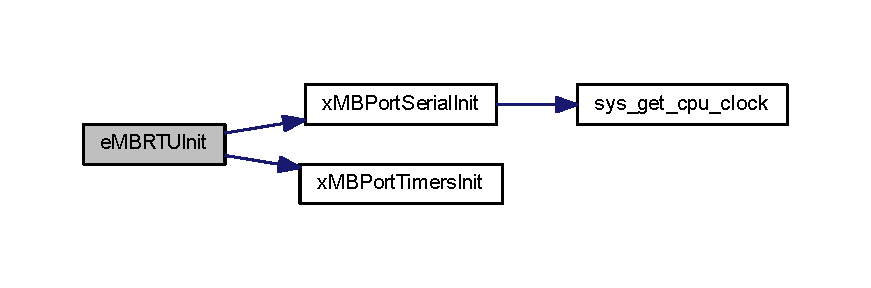
\includegraphics[width=350pt]{mbrtu_8c_a52738b46d7f3be581582d30cfb2bfcb8_cgraph}
\end{center}
\end{figure}




Here is the caller graph for this function\+:
\nopagebreak
\begin{figure}[H]
\begin{center}
\leavevmode
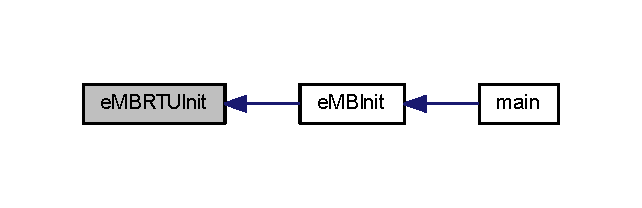
\includegraphics[width=308pt]{mbrtu_8c_a52738b46d7f3be581582d30cfb2bfcb8_icgraph}
\end{center}
\end{figure}


\index{mbrtu.\+c@{mbrtu.\+c}!e\+M\+B\+R\+T\+U\+Start@{e\+M\+B\+R\+T\+U\+Start}}
\index{e\+M\+B\+R\+T\+U\+Start@{e\+M\+B\+R\+T\+U\+Start}!mbrtu.\+c@{mbrtu.\+c}}
\subsubsection[{\texorpdfstring{e\+M\+B\+R\+T\+U\+Start(void)}{eMBRTUStart(void)}}]{\setlength{\rightskip}{0pt plus 5cm}void e\+M\+B\+R\+T\+U\+Start (
\begin{DoxyParamCaption}
\item[{void}]{}
\end{DoxyParamCaption}
)}\hypertarget{mbrtu_8c_ae342bae030ea291a6e8a2fe3d2d0abeb}{}\label{mbrtu_8c_ae342bae030ea291a6e8a2fe3d2d0abeb}


 \subsubsection*{e\+M\+B\+R\+T\+U\+Start }

Event Handler for G\+PI module \begin{DoxyVerb} @date                           DEC/02/2013
 @author                         FW_DEV_2
 @pre                            None
 @return                         None\end{DoxyVerb}
 

Definition at line 151 of file mbrtu.\+c.



Here is the call graph for this function\+:
\nopagebreak
\begin{figure}[H]
\begin{center}
\leavevmode
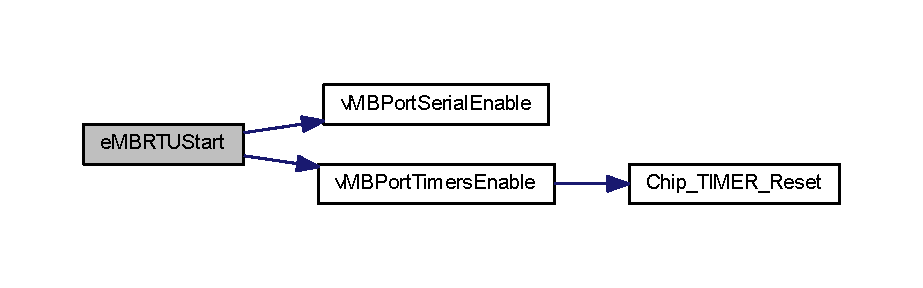
\includegraphics[width=350pt]{mbrtu_8c_ae342bae030ea291a6e8a2fe3d2d0abeb_cgraph}
\end{center}
\end{figure}




Here is the caller graph for this function\+:
\nopagebreak
\begin{figure}[H]
\begin{center}
\leavevmode
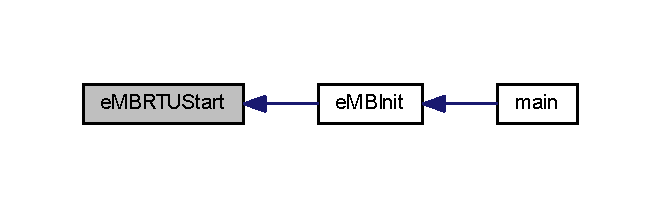
\includegraphics[width=317pt]{mbrtu_8c_ae342bae030ea291a6e8a2fe3d2d0abeb_icgraph}
\end{center}
\end{figure}


\index{mbrtu.\+c@{mbrtu.\+c}!e\+M\+B\+R\+T\+U\+Stop@{e\+M\+B\+R\+T\+U\+Stop}}
\index{e\+M\+B\+R\+T\+U\+Stop@{e\+M\+B\+R\+T\+U\+Stop}!mbrtu.\+c@{mbrtu.\+c}}
\subsubsection[{\texorpdfstring{e\+M\+B\+R\+T\+U\+Stop(void)}{eMBRTUStop(void)}}]{\setlength{\rightskip}{0pt plus 5cm}void e\+M\+B\+R\+T\+U\+Stop (
\begin{DoxyParamCaption}
\item[{void}]{}
\end{DoxyParamCaption}
)}\hypertarget{mbrtu_8c_a3d44ef4747b7202d37142ef1aaea493b}{}\label{mbrtu_8c_a3d44ef4747b7202d37142ef1aaea493b}


 \subsubsection*{e\+M\+B\+R\+T\+U\+Stop }

Event Handler for G\+PI module \begin{DoxyVerb} @date                           DEC/02/2013
 @author                         FW_DEV_2
 @pre                            None
 @return                         None\end{DoxyVerb}
 

Definition at line 179 of file mbrtu.\+c.



Here is the call graph for this function\+:
\nopagebreak
\begin{figure}[H]
\begin{center}
\leavevmode
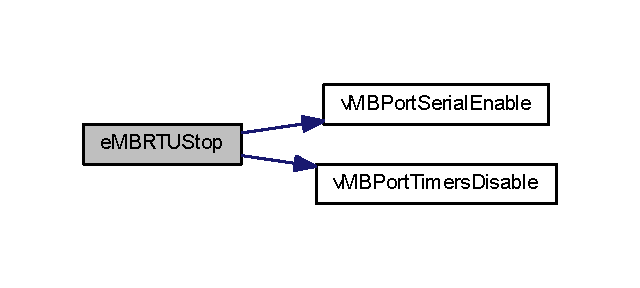
\includegraphics[width=307pt]{mbrtu_8c_a3d44ef4747b7202d37142ef1aaea493b_cgraph}
\end{center}
\end{figure}




Here is the caller graph for this function\+:
\nopagebreak
\begin{figure}[H]
\begin{center}
\leavevmode
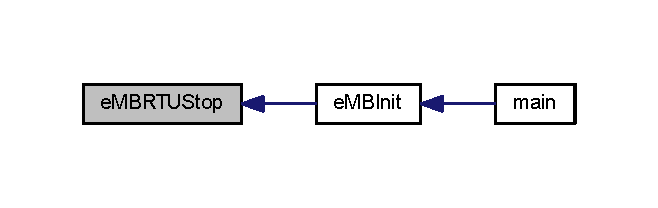
\includegraphics[width=316pt]{mbrtu_8c_a3d44ef4747b7202d37142ef1aaea493b_icgraph}
\end{center}
\end{figure}


\index{mbrtu.\+c@{mbrtu.\+c}!e\+M\+B\+R\+T\+U\+Receive@{e\+M\+B\+R\+T\+U\+Receive}}
\index{e\+M\+B\+R\+T\+U\+Receive@{e\+M\+B\+R\+T\+U\+Receive}!mbrtu.\+c@{mbrtu.\+c}}
\subsubsection[{\texorpdfstring{e\+M\+B\+R\+T\+U\+Receive(\+U\+C\+H\+A\+R $\ast$puc\+Rcv\+Address, U\+C\+H\+A\+R $\ast$$\ast$puc\+Frame, U\+S\+H\+O\+R\+T $\ast$pus\+Length)}{eMBRTUReceive(UCHAR *pucRcvAddress, UCHAR **pucFrame, USHORT *pusLength)}}]{\setlength{\rightskip}{0pt plus 5cm}e\+M\+B\+Error\+Code e\+M\+B\+R\+T\+U\+Receive (
\begin{DoxyParamCaption}
\item[{U\+C\+H\+AR $\ast$}]{puc\+Rcv\+Address, }
\item[{U\+C\+H\+AR $\ast$$\ast$}]{puc\+Frame, }
\item[{U\+S\+H\+O\+RT $\ast$}]{pus\+Length}
\end{DoxyParamCaption}
)}\hypertarget{mbrtu_8c_a669fd79aadbd1cc49ac4f11382dc15d9}{}\label{mbrtu_8c_a669fd79aadbd1cc49ac4f11382dc15d9}


 \subsubsection*{e\+M\+B\+R\+T\+U\+Receive }

Event Handler for G\+PI module \begin{DoxyVerb} @date                           DEC/02/2013
 @author                         FW_DEV_2
 @pre                            None
 @return                         None\end{DoxyVerb}
 

Definition at line 199 of file mbrtu.\+c.



Here is the call graph for this function\+:
\nopagebreak
\begin{figure}[H]
\begin{center}
\leavevmode
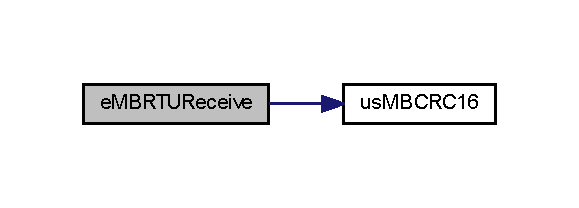
\includegraphics[width=278pt]{mbrtu_8c_a669fd79aadbd1cc49ac4f11382dc15d9_cgraph}
\end{center}
\end{figure}




Here is the caller graph for this function\+:
\nopagebreak
\begin{figure}[H]
\begin{center}
\leavevmode
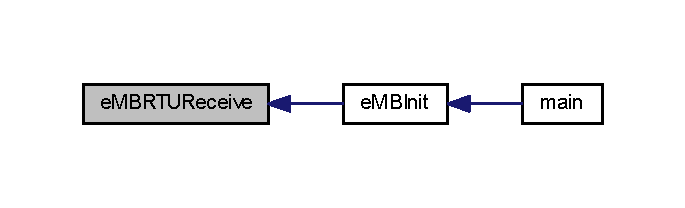
\includegraphics[width=329pt]{mbrtu_8c_a669fd79aadbd1cc49ac4f11382dc15d9_icgraph}
\end{center}
\end{figure}


\index{mbrtu.\+c@{mbrtu.\+c}!e\+M\+B\+R\+T\+U\+Send@{e\+M\+B\+R\+T\+U\+Send}}
\index{e\+M\+B\+R\+T\+U\+Send@{e\+M\+B\+R\+T\+U\+Send}!mbrtu.\+c@{mbrtu.\+c}}
\subsubsection[{\texorpdfstring{e\+M\+B\+R\+T\+U\+Send(\+U\+C\+H\+A\+R uc\+Slave\+Address, const U\+C\+H\+A\+R $\ast$puc\+Frame, U\+S\+H\+O\+R\+T us\+Length)}{eMBRTUSend(UCHAR ucSlaveAddress, const UCHAR *pucFrame, USHORT usLength)}}]{\setlength{\rightskip}{0pt plus 5cm}e\+M\+B\+Error\+Code e\+M\+B\+R\+T\+U\+Send (
\begin{DoxyParamCaption}
\item[{U\+C\+H\+AR}]{uc\+Slave\+Address, }
\item[{const U\+C\+H\+AR $\ast$}]{puc\+Frame, }
\item[{U\+S\+H\+O\+RT}]{us\+Length}
\end{DoxyParamCaption}
)}\hypertarget{mbrtu_8c_a6feb0c70f52d3ef74da1cfbdc10d1ab0}{}\label{mbrtu_8c_a6feb0c70f52d3ef74da1cfbdc10d1ab0}


 \subsubsection*{e\+M\+B\+R\+T\+U\+Send }

Event Handler for G\+PI module \begin{DoxyVerb} @date                           DEC/02/2013
 @author                         FW_DEV_2
 @pre                            None
 @return                         None\end{DoxyVerb}
 

Definition at line 252 of file mbrtu.\+c.



Here is the call graph for this function\+:
\nopagebreak
\begin{figure}[H]
\begin{center}
\leavevmode
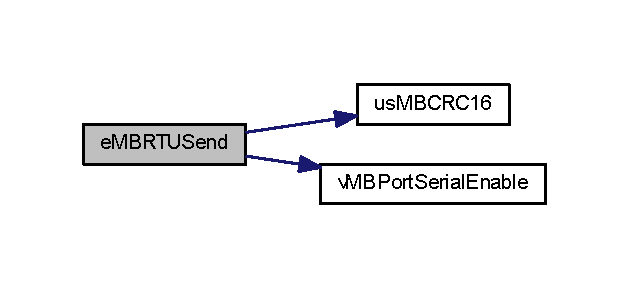
\includegraphics[width=302pt]{mbrtu_8c_a6feb0c70f52d3ef74da1cfbdc10d1ab0_cgraph}
\end{center}
\end{figure}




Here is the caller graph for this function\+:
\nopagebreak
\begin{figure}[H]
\begin{center}
\leavevmode
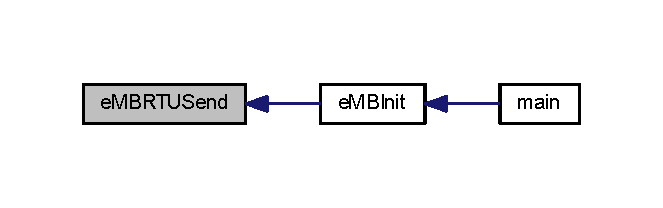
\includegraphics[width=318pt]{mbrtu_8c_a6feb0c70f52d3ef74da1cfbdc10d1ab0_icgraph}
\end{center}
\end{figure}


\index{mbrtu.\+c@{mbrtu.\+c}!x\+M\+B\+R\+T\+U\+Receive\+F\+SM@{x\+M\+B\+R\+T\+U\+Receive\+F\+SM}}
\index{x\+M\+B\+R\+T\+U\+Receive\+F\+SM@{x\+M\+B\+R\+T\+U\+Receive\+F\+SM}!mbrtu.\+c@{mbrtu.\+c}}
\subsubsection[{\texorpdfstring{x\+M\+B\+R\+T\+U\+Receive\+F\+S\+M(void)}{xMBRTUReceiveFSM(void)}}]{\setlength{\rightskip}{0pt plus 5cm}B\+O\+OL x\+M\+B\+R\+T\+U\+Receive\+F\+SM (
\begin{DoxyParamCaption}
\item[{void}]{}
\end{DoxyParamCaption}
)}\hypertarget{mbrtu_8c_a447f45f582daab2600cad612b00120b0}{}\label{mbrtu_8c_a447f45f582daab2600cad612b00120b0}


 \subsubsection*{x\+M\+B\+R\+T\+U\+Receive\+F\+SM }

Event Handler for G\+PI module \begin{DoxyVerb} @date                           DEC/02/2013
 @author                         FW_DEV_2
 @pre                            None
 @return                         None\end{DoxyVerb}
 

Definition at line 302 of file mbrtu.\+c.



Here is the call graph for this function\+:
\nopagebreak
\begin{figure}[H]
\begin{center}
\leavevmode
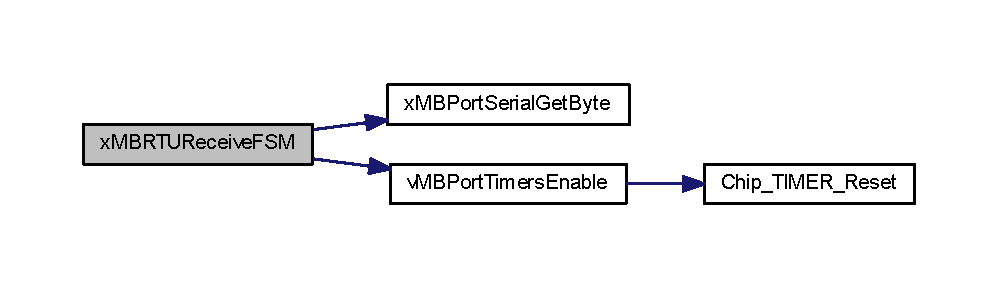
\includegraphics[width=350pt]{mbrtu_8c_a447f45f582daab2600cad612b00120b0_cgraph}
\end{center}
\end{figure}




Here is the caller graph for this function\+:
\nopagebreak
\begin{figure}[H]
\begin{center}
\leavevmode
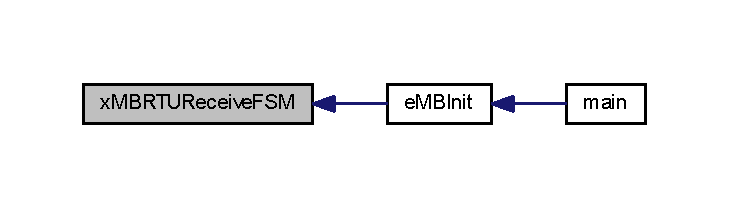
\includegraphics[width=350pt]{mbrtu_8c_a447f45f582daab2600cad612b00120b0_icgraph}
\end{center}
\end{figure}


\index{mbrtu.\+c@{mbrtu.\+c}!x\+M\+B\+R\+T\+U\+Transmit\+F\+SM@{x\+M\+B\+R\+T\+U\+Transmit\+F\+SM}}
\index{x\+M\+B\+R\+T\+U\+Transmit\+F\+SM@{x\+M\+B\+R\+T\+U\+Transmit\+F\+SM}!mbrtu.\+c@{mbrtu.\+c}}
\subsubsection[{\texorpdfstring{x\+M\+B\+R\+T\+U\+Transmit\+F\+S\+M(void)}{xMBRTUTransmitFSM(void)}}]{\setlength{\rightskip}{0pt plus 5cm}B\+O\+OL x\+M\+B\+R\+T\+U\+Transmit\+F\+SM (
\begin{DoxyParamCaption}
\item[{void}]{}
\end{DoxyParamCaption}
)}\hypertarget{mbrtu_8c_a663e5daf0be0f2426a72c531c91d423f}{}\label{mbrtu_8c_a663e5daf0be0f2426a72c531c91d423f}


 \subsubsection*{x\+M\+B\+R\+T\+U\+Transmit\+F\+SM }

Event Handler for G\+PI module \begin{DoxyVerb} @date                           DEC/02/2013
 @author                         FW_DEV_2
 @pre                            None
 @return                         None\end{DoxyVerb}
 

Definition at line 372 of file mbrtu.\+c.



Here is the call graph for this function\+:
\nopagebreak
\begin{figure}[H]
\begin{center}
\leavevmode
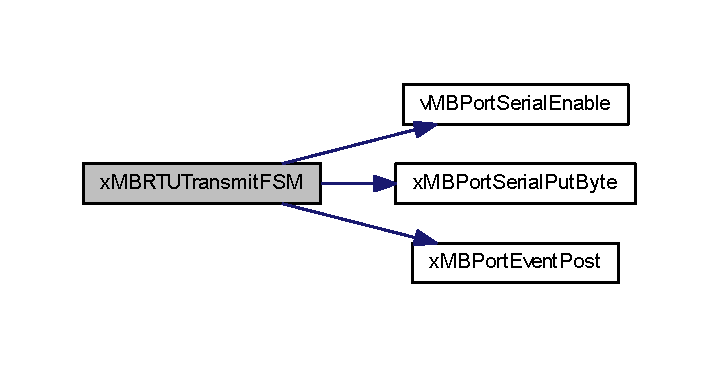
\includegraphics[width=345pt]{mbrtu_8c_a663e5daf0be0f2426a72c531c91d423f_cgraph}
\end{center}
\end{figure}




Here is the caller graph for this function\+:
\nopagebreak
\begin{figure}[H]
\begin{center}
\leavevmode
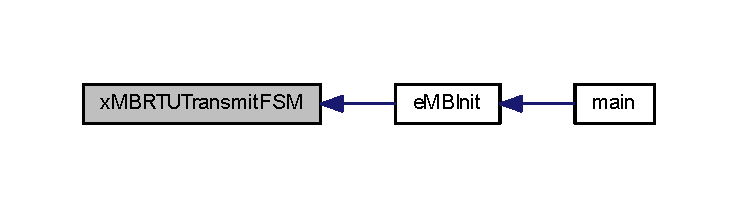
\includegraphics[width=350pt]{mbrtu_8c_a663e5daf0be0f2426a72c531c91d423f_icgraph}
\end{center}
\end{figure}


\index{mbrtu.\+c@{mbrtu.\+c}!x\+M\+B\+R\+T\+U\+Timer\+T35\+Expired@{x\+M\+B\+R\+T\+U\+Timer\+T35\+Expired}}
\index{x\+M\+B\+R\+T\+U\+Timer\+T35\+Expired@{x\+M\+B\+R\+T\+U\+Timer\+T35\+Expired}!mbrtu.\+c@{mbrtu.\+c}}
\subsubsection[{\texorpdfstring{x\+M\+B\+R\+T\+U\+Timer\+T35\+Expired(void)}{xMBRTUTimerT35Expired(void)}}]{\setlength{\rightskip}{0pt plus 5cm}B\+O\+OL x\+M\+B\+R\+T\+U\+Timer\+T35\+Expired (
\begin{DoxyParamCaption}
\item[{void}]{}
\end{DoxyParamCaption}
)}\hypertarget{mbrtu_8c_ac6302a8b67c6b82ae49e6c9d6a9795da}{}\label{mbrtu_8c_ac6302a8b67c6b82ae49e6c9d6a9795da}


 \subsubsection*{x\+M\+B\+R\+T\+U\+Timer\+T35\+Expired }

Event Handler for G\+PI module \begin{DoxyVerb} @date                           DEC/02/2013
 @author                         FW_DEV_2
 @pre                            None
 @return                         None\end{DoxyVerb}
 

Definition at line 420 of file mbrtu.\+c.



Here is the call graph for this function\+:
\nopagebreak
\begin{figure}[H]
\begin{center}
\leavevmode
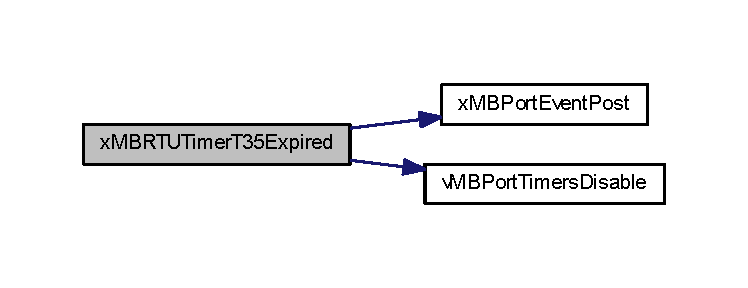
\includegraphics[width=350pt]{mbrtu_8c_ac6302a8b67c6b82ae49e6c9d6a9795da_cgraph}
\end{center}
\end{figure}




Here is the caller graph for this function\+:
\nopagebreak
\begin{figure}[H]
\begin{center}
\leavevmode
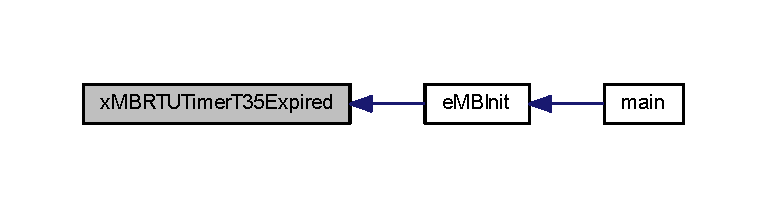
\includegraphics[width=350pt]{mbrtu_8c_ac6302a8b67c6b82ae49e6c9d6a9795da_icgraph}
\end{center}
\end{figure}



\hypertarget{mbutils_8c}{}\section{mbutils.\+c File Reference}
\label{mbutils_8c}\index{mbutils.\+c@{mbutils.\+c}}
{\ttfamily \#include \char`\"{}stdlib.\+h\char`\"{}}\\*
{\ttfamily \#include \char`\"{}string.\+h\char`\"{}}\\*
{\ttfamily \#include \char`\"{}port.\+h\char`\"{}}\\*
{\ttfamily \#include \char`\"{}mb.\+h\char`\"{}}\\*
{\ttfamily \#include \char`\"{}mbproto.\+h\char`\"{}}\\*
{\ttfamily \#include \char`\"{}L\+P\+C17xx.\+h\char`\"{}}\\*
Include dependency graph for mbutils.\+c\+:
\nopagebreak
\begin{figure}[H]
\begin{center}
\leavevmode
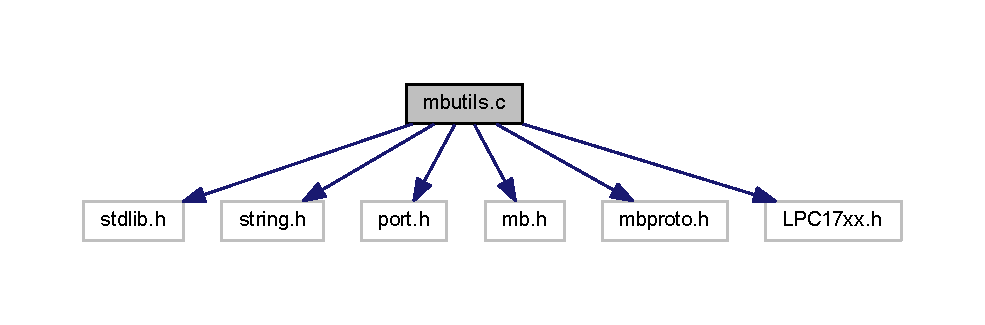
\includegraphics[width=350pt]{mbutils_8c__incl}
\end{center}
\end{figure}
\subsection*{Macros}
\begin{DoxyCompactItemize}
\item 
\#define {\bfseries B\+I\+T\+S\+\_\+\+U\+C\+H\+AR}~8U\hypertarget{mbutils_8c_aad9c8ffbfd788a2a6ba69ed38ea11983}{}\label{mbutils_8c_aad9c8ffbfd788a2a6ba69ed38ea11983}

\item 
\#define \hyperlink{mbutils_8c_a748a344fc38ce1f9469b536aa2663ba0}{I\+N\+T\+E\+R\+N\+A\+L\+\_\+\+C\+L\+O\+CK}~(4  $\ast$ 1000 $\ast$ 1000\+U\+L)\hypertarget{mbutils_8c_a748a344fc38ce1f9469b536aa2663ba0}{}\label{mbutils_8c_a748a344fc38ce1f9469b536aa2663ba0}

\begin{DoxyCompactList}\small\item\em Do not change, this is the same on all L\+P\+C17\+XX. \end{DoxyCompactList}\item 
\#define \hyperlink{mbutils_8c_ae9d5d3d0882e298dbe8f4d5c5152c960}{E\+X\+T\+E\+R\+N\+A\+L\+\_\+\+C\+L\+O\+CK}~(12 $\ast$ 1000 $\ast$ 1000\+U\+L)\hypertarget{mbutils_8c_ae9d5d3d0882e298dbe8f4d5c5152c960}{}\label{mbutils_8c_ae9d5d3d0882e298dbe8f4d5c5152c960}

\begin{DoxyCompactList}\small\item\em Change according to your board specification. \end{DoxyCompactList}\item 
\#define \hyperlink{mbutils_8c_ae359e5fa2f56eadc30656472ac53d174}{R\+T\+C\+\_\+\+C\+L\+O\+CK}~(32768\+U\+L)\hypertarget{mbutils_8c_ae359e5fa2f56eadc30656472ac53d174}{}\label{mbutils_8c_ae359e5fa2f56eadc30656472ac53d174}

\begin{DoxyCompactList}\small\item\em Do not change, this is the typical R\+TC crystal value. \end{DoxyCompactList}\item 
\#define {\bfseries config\+T\+I\+C\+K\+\_\+\+R\+A\+T\+E\+\_\+\+HZ}~( 1000 )\hypertarget{mbutils_8c_a2f0258dd1e3b877e5bc013be54c2db6a}{}\label{mbutils_8c_a2f0258dd1e3b877e5bc013be54c2db6a}

\item 
\#define \hyperlink{mbutils_8c_ab743eff669ae3062b0885a8e0315b641}{O\+S\+\_\+\+MS}(x)~( x / M\+S\+\_\+\+P\+E\+R\+\_\+\+T\+I\+CK() )\hypertarget{mbutils_8c_ab743eff669ae3062b0885a8e0315b641}{}\label{mbutils_8c_ab743eff669ae3062b0885a8e0315b641}

\begin{DoxyCompactList}\small\item\em Ticks to millisecond conversion. \end{DoxyCompactList}\item 
\#define \hyperlink{mbutils_8c_ab743eff669ae3062b0885a8e0315b641}{O\+S\+\_\+\+MS}(x)~( x / M\+S\+\_\+\+P\+E\+R\+\_\+\+T\+I\+CK() )\hypertarget{mbutils_8c_ab743eff669ae3062b0885a8e0315b641}{}\label{mbutils_8c_ab743eff669ae3062b0885a8e0315b641}

\begin{DoxyCompactList}\small\item\em Ticks to millisecond conversion. \end{DoxyCompactList}\end{DoxyCompactItemize}
\subsection*{Functions}
\begin{DoxyCompactItemize}
\item 
void \hyperlink{mbutils_8c_a5e9309bb72bdc5ba7967fd40ae3ca91a}{delay} (uint32\+\_\+t delay\+In\+Ms)
\item 
unsigned int \hyperlink{mbutils_8c_a6ac4b492b79ce75125ae13fd7715873b}{sys\+\_\+get\+\_\+cpu\+\_\+clock} ()
\item 
void \hyperlink{mbutils_8c_a48cf317a6fd966e09ad3afee42dbd866}{x\+M\+B\+Util\+Set\+Bits} (U\+C\+H\+AR $\ast$uc\+Byte\+Buf, U\+S\+H\+O\+RT us\+Bit\+Offset, U\+C\+H\+AR uc\+N\+Bits, U\+C\+H\+AR uc\+Value)
\item 
U\+C\+H\+AR \hyperlink{mbutils_8c_a94b3b43e1d2353e621748c79e2fb4dd5}{x\+M\+B\+Util\+Get\+Bits} (U\+C\+H\+AR $\ast$uc\+Byte\+Buf, U\+S\+H\+O\+RT us\+Bit\+Offset, U\+C\+H\+AR uc\+N\+Bits)
\item 
e\+M\+B\+Exception \hyperlink{mbutils_8c_ad5d2cc07a83fa7ea723ed734c905bc55}{prve\+M\+B\+Error2\+Exception} (e\+M\+B\+Error\+Code e\+Error\+Code)
\end{DoxyCompactItemize}


\subsection{Detailed Description}
Free\+Modbus Libary\+: A portable Modbus implementation for Modbus A\+S\+C\+I\+I/\+R\+TU. Copyright (c) 2006 Christian Walter \href{mailto:wolti@sil.at}{\tt wolti@sil.\+at} All rights reserved.

Redistribution and use in source and binary forms, with or without modification, are permitted provided that the following conditions are met\+:
\begin{DoxyEnumerate}
\item Redistributions of source code must retain the above copyright notice, this list of conditions and the following disclaimer.
\item Redistributions in binary form must reproduce the above copyright notice, this list of conditions and the following disclaimer in the documentation and/or other materials provided with the distribution.
\item The name of the author may not be used to endorse or promote products derived from this software without specific prior written permission.
\end{DoxyEnumerate}

T\+H\+IS S\+O\+F\+T\+W\+A\+RE IS P\+R\+O\+V\+I\+D\+ED BY T\+HE A\+U\+T\+H\+OR ``\+AS IS\textquotesingle{}\textquotesingle{} A\+ND A\+NY E\+X\+P\+R\+E\+SS OR I\+M\+P\+L\+I\+ED W\+A\+R\+R\+A\+N\+T\+I\+ES, I\+N\+C\+L\+U\+D\+I\+NG, B\+UT N\+OT L\+I\+M\+I\+T\+ED TO, T\+HE I\+M\+P\+L\+I\+ED W\+A\+R\+R\+A\+N\+T\+I\+ES OF M\+E\+R\+C\+H\+A\+N\+T\+A\+B\+I\+L\+I\+TY A\+ND F\+I\+T\+N\+E\+SS F\+OR A P\+A\+R\+T\+I\+C\+U\+L\+AR P\+U\+R\+P\+O\+SE A\+RE D\+I\+S\+C\+L\+A\+I\+M\+ED. IN NO E\+V\+E\+NT S\+H\+A\+LL T\+HE A\+U\+T\+H\+OR BE L\+I\+A\+B\+LE F\+OR A\+NY D\+I\+R\+E\+CT, I\+N\+D\+I\+R\+E\+CT, I\+N\+C\+I\+D\+E\+N\+T\+AL, S\+P\+E\+C\+I\+AL, E\+X\+E\+M\+P\+L\+A\+RY, OR C\+O\+N\+S\+E\+Q\+U\+E\+N\+T\+I\+AL D\+A\+M\+A\+G\+ES (I\+N\+C\+L\+U\+D\+I\+NG, B\+UT N\+OT L\+I\+M\+I\+T\+ED TO, P\+R\+O\+C\+U\+R\+E\+M\+E\+NT OF S\+U\+B\+S\+T\+I\+T\+U\+TE G\+O\+O\+DS OR S\+E\+R\+V\+I\+C\+ES; L\+O\+SS OF U\+SE, D\+A\+TA, OR P\+R\+O\+F\+I\+TS; OR B\+U\+S\+I\+N\+E\+SS I\+N\+T\+E\+R\+R\+U\+P\+T\+I\+ON) H\+O\+W\+E\+V\+ER C\+A\+U\+S\+ED A\+ND ON A\+NY T\+H\+E\+O\+RY OF L\+I\+A\+B\+I\+L\+I\+TY, W\+H\+E\+T\+H\+ER IN C\+O\+N\+T\+R\+A\+CT, S\+T\+R\+I\+CT L\+I\+A\+B\+I\+L\+I\+TY, OR T\+O\+RT (I\+N\+C\+L\+U\+D\+I\+NG N\+E\+G\+L\+I\+G\+E\+N\+CE OR O\+T\+H\+E\+R\+W\+I\+SE) A\+R\+I\+S\+I\+NG IN A\+NY W\+AY O\+UT OF T\+HE U\+SE OF T\+H\+IS S\+O\+F\+T\+W\+A\+RE, E\+V\+EN IF A\+D\+V\+I\+S\+ED OF T\+HE P\+O\+S\+S\+I\+B\+I\+L\+I\+TY OF S\+U\+CH D\+A\+M\+A\+GE.

File\+: \begin{DoxyParagraph}{Id}
\hyperlink{mbutils_8c}{mbutils.\+c},v 1.\+6 2007/02/18 23\+:49\+:07 wolti Exp 
\end{DoxyParagraph}


\subsection{Function Documentation}
\index{mbutils.\+c@{mbutils.\+c}!delay@{delay}}
\index{delay@{delay}!mbutils.\+c@{mbutils.\+c}}
\subsubsection[{\texorpdfstring{delay(uint32\+\_\+t delay\+In\+Ms)}{delay(uint32_t delayInMs)}}]{\setlength{\rightskip}{0pt plus 5cm}void delay (
\begin{DoxyParamCaption}
\item[{uint32\+\_\+t}]{delay\+In\+Ms}
\end{DoxyParamCaption}
)}\hypertarget{mbutils_8c_a5e9309bb72bdc5ba7967fd40ae3ca91a}{}\label{mbutils_8c_a5e9309bb72bdc5ba7967fd40ae3ca91a}


 \subsubsection*{delay }

Event Handler for G\+PI module \begin{DoxyVerb} @date                           DEC/02/2013
 @author                         FW_DEV_2
 @pre                            None
 @return                         None\end{DoxyVerb}
 

Definition at line 65 of file mbutils.\+c.

\index{mbutils.\+c@{mbutils.\+c}!sys\+\_\+get\+\_\+cpu\+\_\+clock@{sys\+\_\+get\+\_\+cpu\+\_\+clock}}
\index{sys\+\_\+get\+\_\+cpu\+\_\+clock@{sys\+\_\+get\+\_\+cpu\+\_\+clock}!mbutils.\+c@{mbutils.\+c}}
\subsubsection[{\texorpdfstring{sys\+\_\+get\+\_\+cpu\+\_\+clock()}{sys_get_cpu_clock()}}]{\setlength{\rightskip}{0pt plus 5cm}unsigned int sys\+\_\+get\+\_\+cpu\+\_\+clock (
\begin{DoxyParamCaption}
{}
\end{DoxyParamCaption}
)}\hypertarget{mbutils_8c_a6ac4b492b79ce75125ae13fd7715873b}{}\label{mbutils_8c_a6ac4b492b79ce75125ae13fd7715873b}


 \subsubsection*{sys\+\_\+get\+\_\+cpu\+\_\+clock }

Event Handler for G\+PI module \begin{DoxyVerb} @date                           DEC/02/2013
 @author                         FW_DEV_2
 @pre                            None
 @return                         None\end{DoxyVerb}
 

Definition at line 92 of file mbutils.\+c.



Here is the caller graph for this function\+:
\nopagebreak
\begin{figure}[H]
\begin{center}
\leavevmode
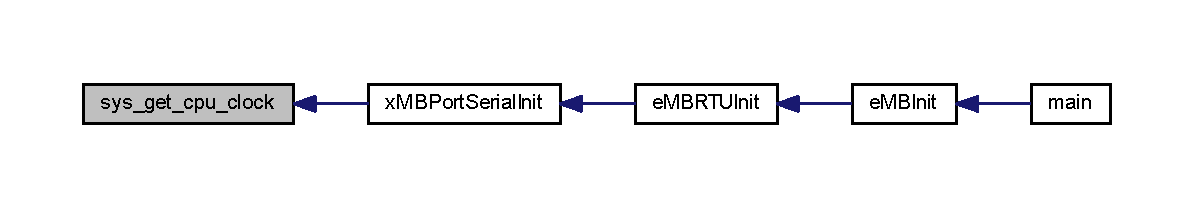
\includegraphics[width=350pt]{mbutils_8c_a6ac4b492b79ce75125ae13fd7715873b_icgraph}
\end{center}
\end{figure}


\index{mbutils.\+c@{mbutils.\+c}!x\+M\+B\+Util\+Set\+Bits@{x\+M\+B\+Util\+Set\+Bits}}
\index{x\+M\+B\+Util\+Set\+Bits@{x\+M\+B\+Util\+Set\+Bits}!mbutils.\+c@{mbutils.\+c}}
\subsubsection[{\texorpdfstring{x\+M\+B\+Util\+Set\+Bits(\+U\+C\+H\+A\+R $\ast$uc\+Byte\+Buf, U\+S\+H\+O\+R\+T us\+Bit\+Offset, U\+C\+H\+A\+R uc\+N\+Bits, U\+C\+H\+A\+R uc\+Value)}{xMBUtilSetBits(UCHAR *ucByteBuf, USHORT usBitOffset, UCHAR ucNBits, UCHAR ucValue)}}]{\setlength{\rightskip}{0pt plus 5cm}void x\+M\+B\+Util\+Set\+Bits (
\begin{DoxyParamCaption}
\item[{U\+C\+H\+AR $\ast$}]{uc\+Byte\+Buf, }
\item[{U\+S\+H\+O\+RT}]{us\+Bit\+Offset, }
\item[{U\+C\+H\+AR}]{uc\+N\+Bits, }
\item[{U\+C\+H\+AR}]{uc\+Value}
\end{DoxyParamCaption}
)}\hypertarget{mbutils_8c_a48cf317a6fd966e09ad3afee42dbd866}{}\label{mbutils_8c_a48cf317a6fd966e09ad3afee42dbd866}


 \subsubsection*{x\+M\+B\+Util\+Set\+Bits }

Event Handler for G\+PI module \begin{DoxyVerb} @date                           DEC/02/2013
 @author                         FW_DEV_2
 @pre                            None
 @return                         None\end{DoxyVerb}
 

Definition at line 158 of file mbutils.\+c.

\index{mbutils.\+c@{mbutils.\+c}!x\+M\+B\+Util\+Get\+Bits@{x\+M\+B\+Util\+Get\+Bits}}
\index{x\+M\+B\+Util\+Get\+Bits@{x\+M\+B\+Util\+Get\+Bits}!mbutils.\+c@{mbutils.\+c}}
\subsubsection[{\texorpdfstring{x\+M\+B\+Util\+Get\+Bits(\+U\+C\+H\+A\+R $\ast$uc\+Byte\+Buf, U\+S\+H\+O\+R\+T us\+Bit\+Offset, U\+C\+H\+A\+R uc\+N\+Bits)}{xMBUtilGetBits(UCHAR *ucByteBuf, USHORT usBitOffset, UCHAR ucNBits)}}]{\setlength{\rightskip}{0pt plus 5cm}U\+C\+H\+AR x\+M\+B\+Util\+Get\+Bits (
\begin{DoxyParamCaption}
\item[{U\+C\+H\+AR $\ast$}]{uc\+Byte\+Buf, }
\item[{U\+S\+H\+O\+RT}]{us\+Bit\+Offset, }
\item[{U\+C\+H\+AR}]{uc\+N\+Bits}
\end{DoxyParamCaption}
)}\hypertarget{mbutils_8c_a94b3b43e1d2353e621748c79e2fb4dd5}{}\label{mbutils_8c_a94b3b43e1d2353e621748c79e2fb4dd5}


 \subsubsection*{x\+M\+B\+Util\+Get\+Bits }

Event Handler for G\+PI module \begin{DoxyVerb} @date                           DEC/02/2013
 @author                         FW_DEV_2
 @pre                            None
 @return                         None\end{DoxyVerb}
 

Definition at line 208 of file mbutils.\+c.

\index{mbutils.\+c@{mbutils.\+c}!prve\+M\+B\+Error2\+Exception@{prve\+M\+B\+Error2\+Exception}}
\index{prve\+M\+B\+Error2\+Exception@{prve\+M\+B\+Error2\+Exception}!mbutils.\+c@{mbutils.\+c}}
\subsubsection[{\texorpdfstring{prve\+M\+B\+Error2\+Exception(e\+M\+B\+Error\+Code e\+Error\+Code)}{prveMBError2Exception(eMBErrorCode eErrorCode)}}]{\setlength{\rightskip}{0pt plus 5cm}e\+M\+B\+Exception prve\+M\+B\+Error2\+Exception (
\begin{DoxyParamCaption}
\item[{e\+M\+B\+Error\+Code}]{e\+Error\+Code}
\end{DoxyParamCaption}
)}\hypertarget{mbutils_8c_ad5d2cc07a83fa7ea723ed734c905bc55}{}\label{mbutils_8c_ad5d2cc07a83fa7ea723ed734c905bc55}


 \subsubsection*{prve\+M\+B\+Error2\+Exception }

Event Handler for G\+PI module \begin{DoxyVerb} @date                           DEC/02/2013
 @author                         FW_DEV_2
 @pre                            None
 @return                         None\end{DoxyVerb}
 

Definition at line 249 of file mbutils.\+c.


\hypertarget{modbus_8c}{}\section{modbus.\+c File Reference}
\label{modbus_8c}\index{modbus.\+c@{modbus.\+c}}
{\ttfamily \#include $<$cr\+\_\+section\+\_\+macros.\+h$>$}\\*
{\ttfamily \#include $<$stdio.\+h$>$}\\*
{\ttfamily \#include $<$stdlib.\+h$>$}\\*
{\ttfamily \#include $<$math.\+h$>$}\\*
{\ttfamily \#include \char`\"{}extint.\+h\char`\"{}}\\*
{\ttfamily \#include \char`\"{}timer.\+h\char`\"{}}\\*
{\ttfamily \#include \char`\"{}L\+P\+C17xx.\+h\char`\"{}}\\*
{\ttfamily \#include $<$string.\+h$>$}\\*
{\ttfamily \#include $<$stdbool.\+h$>$}\\*
Include dependency graph for modbus.\+c\+:
\nopagebreak
\begin{figure}[H]
\begin{center}
\leavevmode
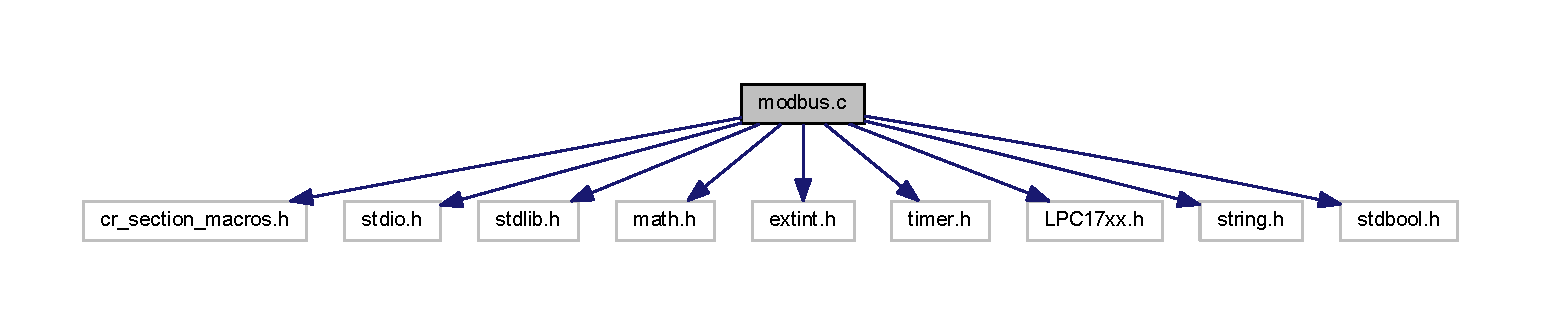
\includegraphics[width=350pt]{modbus_8c__incl}
\end{center}
\end{figure}
\subsection*{Macros}
\begin{DoxyCompactItemize}
\item 
\#define \hyperlink{modbus_8c_a748a344fc38ce1f9469b536aa2663ba0}{I\+N\+T\+E\+R\+N\+A\+L\+\_\+\+C\+L\+O\+CK}~(4  $\ast$ 1000 $\ast$ 1000\+U\+L)\hypertarget{modbus_8c_a748a344fc38ce1f9469b536aa2663ba0}{}\label{modbus_8c_a748a344fc38ce1f9469b536aa2663ba0}

\begin{DoxyCompactList}\small\item\em Do not change, this is the same on all L\+P\+C17\+XX. \end{DoxyCompactList}\item 
\#define \hyperlink{modbus_8c_ae9d5d3d0882e298dbe8f4d5c5152c960}{E\+X\+T\+E\+R\+N\+A\+L\+\_\+\+C\+L\+O\+CK}~(12 $\ast$ 1000 $\ast$ 1000\+U\+L)\hypertarget{modbus_8c_ae9d5d3d0882e298dbe8f4d5c5152c960}{}\label{modbus_8c_ae9d5d3d0882e298dbe8f4d5c5152c960}

\begin{DoxyCompactList}\small\item\em Change according to your board specification. \end{DoxyCompactList}\item 
\#define \hyperlink{modbus_8c_ae359e5fa2f56eadc30656472ac53d174}{R\+T\+C\+\_\+\+C\+L\+O\+CK}~(32768\+U\+L)\hypertarget{modbus_8c_ae359e5fa2f56eadc30656472ac53d174}{}\label{modbus_8c_ae359e5fa2f56eadc30656472ac53d174}

\begin{DoxyCompactList}\small\item\em Do not change, this is the typical R\+TC crystal value. \end{DoxyCompactList}\item 
\#define {\bfseries config\+T\+I\+C\+K\+\_\+\+R\+A\+T\+E\+\_\+\+HZ}~( 1000 )\hypertarget{modbus_8c_a2f0258dd1e3b877e5bc013be54c2db6a}{}\label{modbus_8c_a2f0258dd1e3b877e5bc013be54c2db6a}

\item 
\#define \hyperlink{modbus_8c_ab743eff669ae3062b0885a8e0315b641}{O\+S\+\_\+\+MS}(x)~( x / M\+S\+\_\+\+P\+E\+R\+\_\+\+T\+I\+CK() )\hypertarget{modbus_8c_ab743eff669ae3062b0885a8e0315b641}{}\label{modbus_8c_ab743eff669ae3062b0885a8e0315b641}

\begin{DoxyCompactList}\small\item\em Ticks to millisecond conversion. \end{DoxyCompactList}\item 
\#define \hyperlink{modbus_8c_ab743eff669ae3062b0885a8e0315b641}{O\+S\+\_\+\+MS}(x)~( x / M\+S\+\_\+\+P\+E\+R\+\_\+\+T\+I\+CK() )\hypertarget{modbus_8c_ab743eff669ae3062b0885a8e0315b641}{}\label{modbus_8c_ab743eff669ae3062b0885a8e0315b641}

\begin{DoxyCompactList}\small\item\em Ticks to millisecond conversion. \end{DoxyCompactList}\end{DoxyCompactItemize}
\subsection*{Variables}
\begin{DoxyCompactItemize}
\item 
char {\bfseries Read\+Char}\hypertarget{modbus_8c_a251e2c50e0ea1ca3a2b59c99348e8718}{}\label{modbus_8c_a251e2c50e0ea1ca3a2b59c99348e8718}

\end{DoxyCompactItemize}


\subsection{Detailed Description}
Author \+:  Version \+: Copyright \+:  \subsection*{Description \+: main definition }
\hypertarget{portevent_8c}{}\section{portevent.\+c File Reference}
\label{portevent_8c}\index{portevent.\+c@{portevent.\+c}}


This is main source file for G\+PI Module.  


{\ttfamily \#include \char`\"{}mb.\+h\char`\"{}}\\*
{\ttfamily \#include \char`\"{}mbport.\+h\char`\"{}}\\*
Include dependency graph for portevent.\+c\+:\nopagebreak
\begin{figure}[H]
\begin{center}
\leavevmode
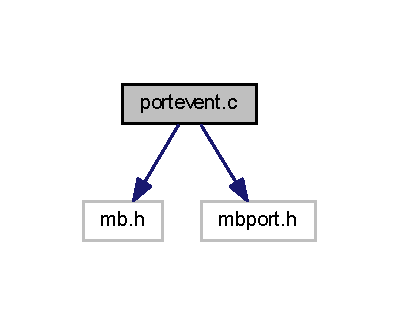
\includegraphics[width=192pt]{portevent_8c__incl}
\end{center}
\end{figure}
\subsection*{Functions}
\begin{DoxyCompactItemize}
\item 
B\+O\+OL {\bfseries x\+M\+B\+Port\+Event\+Init} (void)\hypertarget{portevent_8c_a23aa6afd41597f7aaf5d1a6e6831c718}{}\label{portevent_8c_a23aa6afd41597f7aaf5d1a6e6831c718}

\item 
B\+O\+OL \hyperlink{portevent_8c_a2cdfe42cd5ee37d5839081c636576e7c}{x\+M\+B\+Port\+Event\+Post} (e\+M\+B\+Event\+Type e\+Event)
\item 
B\+O\+OL \hyperlink{portevent_8c_ad61d350e63d0c41e7563ac0bc0fd346f}{x\+M\+B\+Port\+Event\+Get} (e\+M\+B\+Event\+Type $\ast$e\+Event)
\end{DoxyCompactItemize}


\subsection{Detailed Description}
This is main source file for G\+PI Module. 

===============================================================================

Free\+Modbus Libary\+: B\+A\+RE Port Copyright (C) 2006 Christian Walter \href{mailto:wolti@sil.at}{\tt wolti@sil.\+at}

This library is free software; you can redistribute it and/or modify it under the terms of the G\+NU Lesser General Public License as published by the Free Software Foundation; either version 2.\+1 of the License, or (at your option) any later version.

This library is distributed in the hope that it will be useful, but W\+I\+T\+H\+O\+UT A\+NY W\+A\+R\+R\+A\+N\+TY; without even the implied warranty of M\+E\+R\+C\+H\+A\+N\+T\+A\+B\+I\+L\+I\+TY or F\+I\+T\+N\+E\+SS F\+OR A P\+A\+R\+T\+I\+C\+U\+L\+AR P\+U\+R\+P\+O\+SE. See the G\+NU Lesser General Public License for more details.

You should have received a copy of the G\+NU Lesser General Public License along with this library; if not, write to the Free Software Foundation, Inc., 51 Franklin St, Fifth Floor, Boston, MA 02110-\/1301 U\+SA

File\+: \begin{DoxyParagraph}{Id}
\hyperlink{portevent_8c}{portevent.\+c},v 1.\+1 2006/08/22 21\+:35\+:13 wolti Exp 
\end{DoxyParagraph}


\subsection{Function Documentation}
\index{portevent.\+c@{portevent.\+c}!x\+M\+B\+Port\+Event\+Post@{x\+M\+B\+Port\+Event\+Post}}
\index{x\+M\+B\+Port\+Event\+Post@{x\+M\+B\+Port\+Event\+Post}!portevent.\+c@{portevent.\+c}}
\subsubsection[{\texorpdfstring{x\+M\+B\+Port\+Event\+Post(e\+M\+B\+Event\+Type e\+Event)}{xMBPortEventPost(eMBEventType eEvent)}}]{\setlength{\rightskip}{0pt plus 5cm}B\+O\+OL x\+M\+B\+Port\+Event\+Post (
\begin{DoxyParamCaption}
\item[{e\+M\+B\+Event\+Type}]{e\+Event}
\end{DoxyParamCaption}
)}\hypertarget{portevent_8c_a2cdfe42cd5ee37d5839081c636576e7c}{}\label{portevent_8c_a2cdfe42cd5ee37d5839081c636576e7c}


 \subsubsection*{x\+M\+B\+Port\+Event\+Post }

Event Handler for G\+PI module \begin{DoxyVerb} @date                           DEC/02/2013
 @author                         FW_DEV_2
 @pre                            None
 @return                         None\end{DoxyVerb}
 

Definition at line 52 of file portevent.\+c.



Here is the caller graph for this function\+:
\nopagebreak
\begin{figure}[H]
\begin{center}
\leavevmode
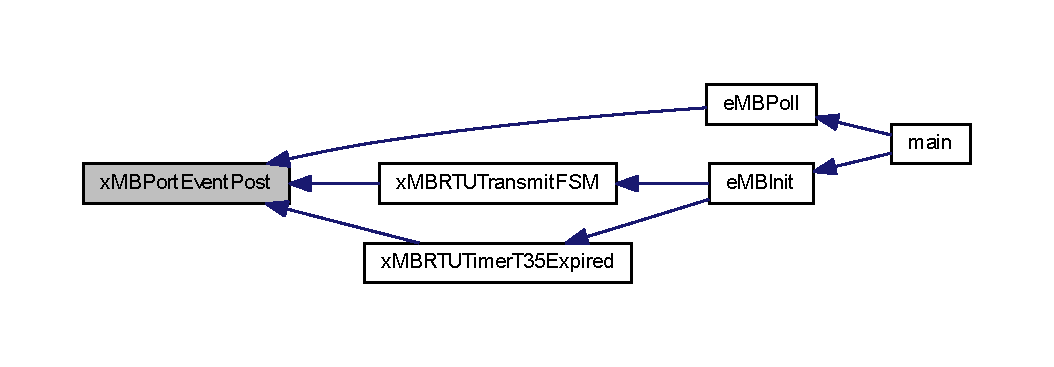
\includegraphics[width=350pt]{portevent_8c_a2cdfe42cd5ee37d5839081c636576e7c_icgraph}
\end{center}
\end{figure}


\index{portevent.\+c@{portevent.\+c}!x\+M\+B\+Port\+Event\+Get@{x\+M\+B\+Port\+Event\+Get}}
\index{x\+M\+B\+Port\+Event\+Get@{x\+M\+B\+Port\+Event\+Get}!portevent.\+c@{portevent.\+c}}
\subsubsection[{\texorpdfstring{x\+M\+B\+Port\+Event\+Get(e\+M\+B\+Event\+Type $\ast$e\+Event)}{xMBPortEventGet(eMBEventType *eEvent)}}]{\setlength{\rightskip}{0pt plus 5cm}B\+O\+OL x\+M\+B\+Port\+Event\+Get (
\begin{DoxyParamCaption}
\item[{e\+M\+B\+Event\+Type $\ast$}]{e\+Event}
\end{DoxyParamCaption}
)}\hypertarget{portevent_8c_ad61d350e63d0c41e7563ac0bc0fd346f}{}\label{portevent_8c_ad61d350e63d0c41e7563ac0bc0fd346f}


 \subsubsection*{x\+M\+B\+Port\+Event\+Get }

Event Handler for G\+PI module \begin{DoxyVerb} @date                           DEC/02/2013
 @author                         FW_DEV_2
 @pre                            None
 @return                         None\end{DoxyVerb}
 

Definition at line 71 of file portevent.\+c.



Here is the caller graph for this function\+:
\nopagebreak
\begin{figure}[H]
\begin{center}
\leavevmode
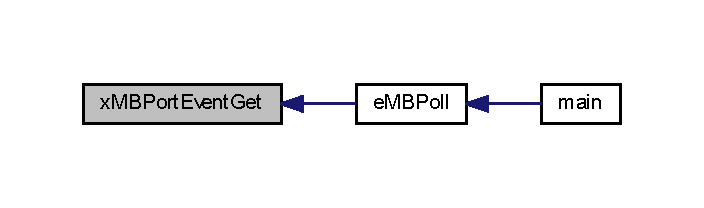
\includegraphics[width=338pt]{portevent_8c_ad61d350e63d0c41e7563ac0bc0fd346f_icgraph}
\end{center}
\end{figure}



\hypertarget{portserial_8c}{}\section{portserial.\+c File Reference}
\label{portserial_8c}\index{portserial.\+c@{portserial.\+c}}
{\ttfamily \#include \char`\"{}port.\+h\char`\"{}}\\*
{\ttfamily \#include \char`\"{}mb.\+h\char`\"{}}\\*
{\ttfamily \#include \char`\"{}mbport.\+h\char`\"{}}\\*
{\ttfamily \#include \char`\"{}L\+P\+C17xx.\+h\char`\"{}}\\*
{\ttfamily \#include \char`\"{}portserial.\+h\char`\"{}}\\*
{\ttfamily \#include \char`\"{}mbutils.\+h\char`\"{}}\\*
Include dependency graph for portserial.\+c\+:
\nopagebreak
\begin{figure}[H]
\begin{center}
\leavevmode
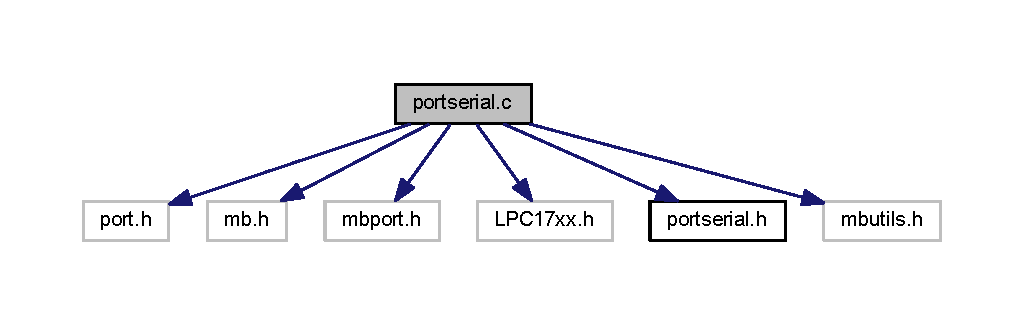
\includegraphics[width=350pt]{portserial_8c__incl}
\end{center}
\end{figure}
\subsection*{Functions}
\begin{DoxyCompactItemize}
\item 
void \hyperlink{portserial_8c_a4bf68bda6b5ed6c341d27d439a6c03df}{v\+M\+B\+Port\+Serial\+Enable} (B\+O\+OL x\+Rx\+Enable, B\+O\+OL x\+Tx\+Enable)
\item 
B\+O\+OL \hyperlink{portserial_8c_a34627006710d0ea50c9215afad55ed55}{x\+M\+B\+Port\+Serial\+Init} (U\+C\+H\+AR uc\+P\+O\+RT, U\+L\+O\+NG ul\+Baud\+Rate, U\+C\+H\+AR uc\+Data\+Bits, e\+M\+B\+Parity e\+Parity)
\item 
B\+O\+OL \hyperlink{portserial_8c_a5ca95563c25eb239a4c51f3ce35f5cc8}{x\+M\+B\+Port\+Serial\+Put\+Byte} (C\+H\+AR uc\+Byte)
\item 
B\+O\+OL \hyperlink{portserial_8c_a4a4724e9dc26b2d2d1cc2a6d41c24770}{x\+M\+B\+Port\+Serial\+Get\+Byte} (C\+H\+AR $\ast$puc\+Byte)
\end{DoxyCompactItemize}


\subsection{Detailed Description}
Free\+Modbus Libary\+: B\+A\+RE Port Copyright (C) 2006 Christian Walter \href{mailto:wolti@sil.at}{\tt wolti@sil.\+at}

This library is free software; you can redistribute it and/or modify it under the terms of the G\+NU Lesser General Public License as published by the Free Software Foundation; either version 2.\+1 of the License, or (at your option) any later version.

This library is distributed in the hope that it will be useful, but W\+I\+T\+H\+O\+UT A\+NY W\+A\+R\+R\+A\+N\+TY; without even the implied warranty of M\+E\+R\+C\+H\+A\+N\+T\+A\+B\+I\+L\+I\+TY or F\+I\+T\+N\+E\+SS F\+OR A P\+A\+R\+T\+I\+C\+U\+L\+AR P\+U\+R\+P\+O\+SE. See the G\+NU Lesser General Public License for more details.

You should have received a copy of the G\+NU Lesser General Public License along with this library; if not, write to the Free Software Foundation, Inc., 51 Franklin St, Fifth Floor, Boston, MA 02110-\/1301 U\+SA

File\+: \begin{DoxyParagraph}{Id}
\hyperlink{portserial_8c}{portserial.\+c},v 1.\+1 2006/08/22 21\+:35\+:13 wolti Exp 
\end{DoxyParagraph}


\subsection{Function Documentation}
\index{portserial.\+c@{portserial.\+c}!v\+M\+B\+Port\+Serial\+Enable@{v\+M\+B\+Port\+Serial\+Enable}}
\index{v\+M\+B\+Port\+Serial\+Enable@{v\+M\+B\+Port\+Serial\+Enable}!portserial.\+c@{portserial.\+c}}
\subsubsection[{\texorpdfstring{v\+M\+B\+Port\+Serial\+Enable(\+B\+O\+O\+L x\+Rx\+Enable, B\+O\+O\+L x\+Tx\+Enable)}{vMBPortSerialEnable(BOOL xRxEnable, BOOL xTxEnable)}}]{\setlength{\rightskip}{0pt plus 5cm}void v\+M\+B\+Port\+Serial\+Enable (
\begin{DoxyParamCaption}
\item[{B\+O\+OL}]{x\+Rx\+Enable, }
\item[{B\+O\+OL}]{x\+Tx\+Enable}
\end{DoxyParamCaption}
)}\hypertarget{portserial_8c_a4bf68bda6b5ed6c341d27d439a6c03df}{}\label{portserial_8c_a4bf68bda6b5ed6c341d27d439a6c03df}


 \subsubsection*{v\+M\+B\+Port\+Serial\+Enable }

Event Handler for G\+PI module \begin{DoxyVerb} @date                           DEC/02/2013
 @author                         FW_DEV_2
 @pre                            None
 @return                         None\end{DoxyVerb}
 

Definition at line 99 of file portserial.\+c.



Here is the caller graph for this function\+:
\nopagebreak
\begin{figure}[H]
\begin{center}
\leavevmode
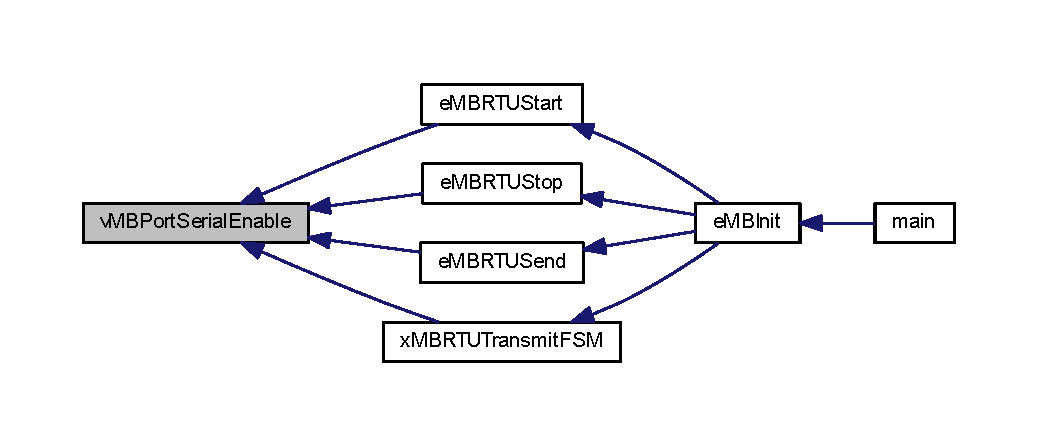
\includegraphics[width=350pt]{portserial_8c_a4bf68bda6b5ed6c341d27d439a6c03df_icgraph}
\end{center}
\end{figure}


\index{portserial.\+c@{portserial.\+c}!x\+M\+B\+Port\+Serial\+Init@{x\+M\+B\+Port\+Serial\+Init}}
\index{x\+M\+B\+Port\+Serial\+Init@{x\+M\+B\+Port\+Serial\+Init}!portserial.\+c@{portserial.\+c}}
\subsubsection[{\texorpdfstring{x\+M\+B\+Port\+Serial\+Init(\+U\+C\+H\+A\+R uc\+P\+O\+R\+T, U\+L\+O\+N\+G ul\+Baud\+Rate, U\+C\+H\+A\+R uc\+Data\+Bits, e\+M\+B\+Parity e\+Parity)}{xMBPortSerialInit(UCHAR ucPORT, ULONG ulBaudRate, UCHAR ucDataBits, eMBParity eParity)}}]{\setlength{\rightskip}{0pt plus 5cm}B\+O\+OL x\+M\+B\+Port\+Serial\+Init (
\begin{DoxyParamCaption}
\item[{U\+C\+H\+AR}]{uc\+P\+O\+RT, }
\item[{U\+L\+O\+NG}]{ul\+Baud\+Rate, }
\item[{U\+C\+H\+AR}]{uc\+Data\+Bits, }
\item[{e\+M\+B\+Parity}]{e\+Parity}
\end{DoxyParamCaption}
)}\hypertarget{portserial_8c_a34627006710d0ea50c9215afad55ed55}{}\label{portserial_8c_a34627006710d0ea50c9215afad55ed55}


 \subsubsection*{x\+M\+B\+Port\+Serial\+Init }

Event Handler for G\+PI module \begin{DoxyVerb} @date                           DEC/02/2013
 @author                         FW_DEV_2
 @pre                            None
 @return                         None\end{DoxyVerb}
 

Definition at line 120 of file portserial.\+c.



Here is the call graph for this function\+:
\nopagebreak
\begin{figure}[H]
\begin{center}
\leavevmode
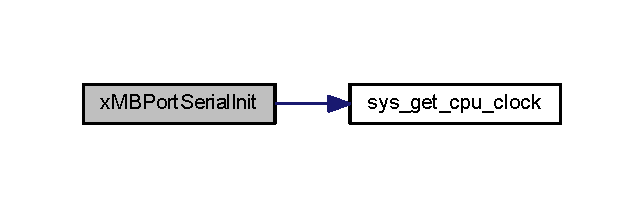
\includegraphics[width=309pt]{portserial_8c_a34627006710d0ea50c9215afad55ed55_cgraph}
\end{center}
\end{figure}




Here is the caller graph for this function\+:
\nopagebreak
\begin{figure}[H]
\begin{center}
\leavevmode
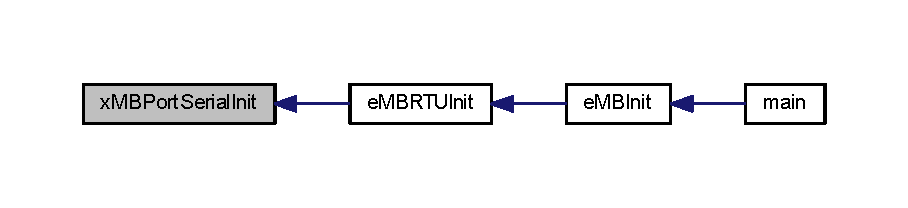
\includegraphics[width=350pt]{portserial_8c_a34627006710d0ea50c9215afad55ed55_icgraph}
\end{center}
\end{figure}


\index{portserial.\+c@{portserial.\+c}!x\+M\+B\+Port\+Serial\+Put\+Byte@{x\+M\+B\+Port\+Serial\+Put\+Byte}}
\index{x\+M\+B\+Port\+Serial\+Put\+Byte@{x\+M\+B\+Port\+Serial\+Put\+Byte}!portserial.\+c@{portserial.\+c}}
\subsubsection[{\texorpdfstring{x\+M\+B\+Port\+Serial\+Put\+Byte(\+C\+H\+A\+R uc\+Byte)}{xMBPortSerialPutByte(CHAR ucByte)}}]{\setlength{\rightskip}{0pt plus 5cm}B\+O\+OL x\+M\+B\+Port\+Serial\+Put\+Byte (
\begin{DoxyParamCaption}
\item[{C\+H\+AR}]{uc\+Byte}
\end{DoxyParamCaption}
)}\hypertarget{portserial_8c_a5ca95563c25eb239a4c51f3ce35f5cc8}{}\label{portserial_8c_a5ca95563c25eb239a4c51f3ce35f5cc8}


 \subsubsection*{x\+M\+B\+Port\+Serial\+Put\+Byte }

Event Handler for G\+PI module \begin{DoxyVerb} @date                           DEC/02/2013
 @author                         FW_DEV_2
 @pre                            None
 @return                         None\end{DoxyVerb}
 

Definition at line 185 of file portserial.\+c.



Here is the caller graph for this function\+:
\nopagebreak
\begin{figure}[H]
\begin{center}
\leavevmode
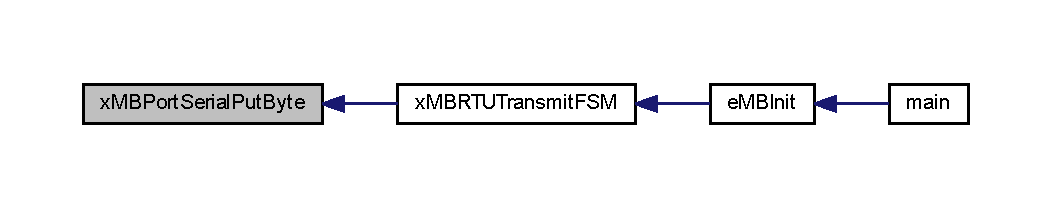
\includegraphics[width=350pt]{portserial_8c_a5ca95563c25eb239a4c51f3ce35f5cc8_icgraph}
\end{center}
\end{figure}


\index{portserial.\+c@{portserial.\+c}!x\+M\+B\+Port\+Serial\+Get\+Byte@{x\+M\+B\+Port\+Serial\+Get\+Byte}}
\index{x\+M\+B\+Port\+Serial\+Get\+Byte@{x\+M\+B\+Port\+Serial\+Get\+Byte}!portserial.\+c@{portserial.\+c}}
\subsubsection[{\texorpdfstring{x\+M\+B\+Port\+Serial\+Get\+Byte(\+C\+H\+A\+R $\ast$puc\+Byte)}{xMBPortSerialGetByte(CHAR *pucByte)}}]{\setlength{\rightskip}{0pt plus 5cm}B\+O\+OL x\+M\+B\+Port\+Serial\+Get\+Byte (
\begin{DoxyParamCaption}
\item[{C\+H\+AR $\ast$}]{puc\+Byte}
\end{DoxyParamCaption}
)}\hypertarget{portserial_8c_a4a4724e9dc26b2d2d1cc2a6d41c24770}{}\label{portserial_8c_a4a4724e9dc26b2d2d1cc2a6d41c24770}


 \subsubsection*{x\+M\+B\+Port\+Serial\+Get\+Byte }

Event Handler for G\+PI module \begin{DoxyVerb} @date                           DEC/02/2013
 @author                         FW_DEV_2
 @pre                            None
 @return                         None\end{DoxyVerb}
 

Definition at line 209 of file portserial.\+c.



Here is the caller graph for this function\+:
\nopagebreak
\begin{figure}[H]
\begin{center}
\leavevmode
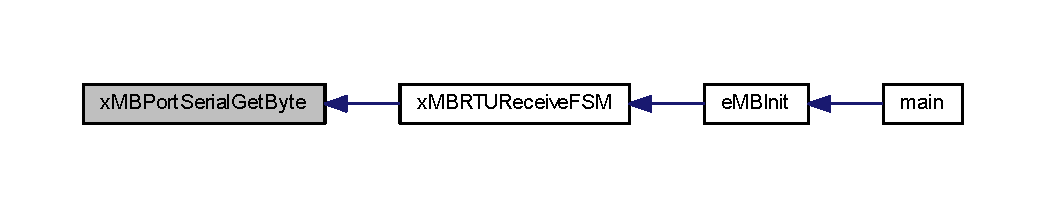
\includegraphics[width=350pt]{portserial_8c_a4a4724e9dc26b2d2d1cc2a6d41c24770_icgraph}
\end{center}
\end{figure}



\hypertarget{portserial_8h}{}\section{portserial.\+h File Reference}
\label{portserial_8h}\index{portserial.\+h@{portserial.\+h}}
This graph shows which files directly or indirectly include this file\+:
\nopagebreak
\begin{figure}[H]
\begin{center}
\leavevmode
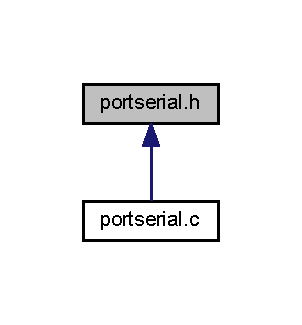
\includegraphics[width=145pt]{portserial_8h__dep__incl}
\end{center}
\end{figure}
\subsection*{Macros}
\begin{DoxyCompactItemize}
\item 
\#define \hyperlink{portserial_8h_a1592b78e87967ae6a06756679cfc855e}{U\+A\+R\+T\+\_\+\+T\+H\+R\+\_\+\+M\+A\+S\+K\+B\+IT}~((uint8\+\_\+t)0x\+F\+F)
\item 
\#define \hyperlink{portserial_8h_ab5fadcd32fca709aece83c05f8be1901}{U\+A\+R\+T\+\_\+\+I\+I\+R\+\_\+\+I\+N\+T\+S\+T\+A\+T\+\_\+\+P\+E\+ND}~((uint32\+\_\+t)(1$<$$<$0))
\item 
\#define \hyperlink{portserial_8h_a4441660d2a99f6b17a79eafbfb0424dd}{U\+A\+R\+T\+\_\+\+I\+I\+R\+\_\+\+I\+N\+T\+I\+D\+\_\+\+R\+LS}~((uint32\+\_\+t)(3$<$$<$1))
\item 
\#define \hyperlink{portserial_8h_ac646d8f797f3e71e01f4361997fc581b}{U\+A\+R\+T\+\_\+\+I\+I\+R\+\_\+\+I\+N\+T\+I\+D\+\_\+\+R\+DA}~((uint32\+\_\+t)(2$<$$<$1))
\item 
\#define \hyperlink{portserial_8h_a965ba229214955385f11277549b7ecce}{U\+A\+R\+T\+\_\+\+I\+I\+R\+\_\+\+I\+N\+T\+I\+D\+\_\+\+C\+TI}~((uint32\+\_\+t)(6$<$$<$1))
\item 
\#define \hyperlink{portserial_8h_afb93160677afbc9c90f7a0baa917a435}{U\+A\+R\+T\+\_\+\+I\+I\+R\+\_\+\+I\+N\+T\+I\+D\+\_\+\+T\+H\+RE}~((uint32\+\_\+t)(1$<$$<$1))
\item 
\#define \hyperlink{portserial_8h_a0496801d1096f782e06e6d394836db91}{U\+A\+R\+T1\+\_\+\+I\+I\+R\+\_\+\+I\+N\+T\+I\+D\+\_\+\+M\+O\+D\+EM}~((uint32\+\_\+t)(0$<$$<$1))
\item 
\#define \hyperlink{portserial_8h_a6f78952aec5835ac753718323b681910}{U\+A\+R\+T\+\_\+\+I\+I\+R\+\_\+\+I\+N\+T\+I\+D\+\_\+\+M\+A\+SK}~((uint32\+\_\+t)(7$<$$<$1))
\item 
\#define \hyperlink{portserial_8h_a29b20e73585acb416f112502d29554d7}{U\+A\+R\+T\+\_\+\+I\+I\+R\+\_\+\+F\+I\+F\+O\+\_\+\+EN}~((uint32\+\_\+t)(3$<$$<$6))
\item 
\#define \hyperlink{portserial_8h_a6ce7f02b02e196d84ef8f6066dd2b9d4}{U\+A\+R\+T\+\_\+\+I\+I\+R\+\_\+\+A\+B\+E\+O\+\_\+\+I\+NT}~((uint32\+\_\+t)(1$<$$<$8))
\item 
\#define \hyperlink{portserial_8h_a29486c78b0afdb4b3943defe36d5404c}{U\+A\+R\+T\+\_\+\+I\+I\+R\+\_\+\+A\+B\+T\+O\+\_\+\+I\+NT}~((uint32\+\_\+t)(1$<$$<$9))
\item 
\#define \hyperlink{portserial_8h_ad443b74131fa7b7aecf0f1c581172faa}{U\+A\+R\+T\+\_\+\+I\+I\+R\+\_\+\+B\+I\+T\+M\+A\+SK}~((uint32\+\_\+t)(0x3\+C\+F))
\item 
\#define \hyperlink{portserial_8h_a3d83de31d722cd373ee69a2a38aaed43}{U\+A\+R\+T\+\_\+\+L\+S\+R\+\_\+\+R\+DR}~((uint8\+\_\+t)(1$<$$<$0))
\item 
\#define \hyperlink{portserial_8h_a85c4312a700f6033bf0a075ae41de57c}{U\+A\+R\+T\+\_\+\+L\+S\+R\+\_\+\+OE}~((uint8\+\_\+t)(1$<$$<$1))
\item 
\#define \hyperlink{portserial_8h_a3ae0ee26be22b855aa08d68a2801d3d2}{U\+A\+R\+T\+\_\+\+L\+S\+R\+\_\+\+PE}~((uint8\+\_\+t)(1$<$$<$2))
\item 
\#define \hyperlink{portserial_8h_a18b1661d7c37ab40c9310311dd4f647d}{U\+A\+R\+T\+\_\+\+L\+S\+R\+\_\+\+FE}~((uint8\+\_\+t)(1$<$$<$3))
\item 
\#define \hyperlink{portserial_8h_aaca4bb43e62c7085534b67576e1ddbeb}{U\+A\+R\+T\+\_\+\+L\+S\+R\+\_\+\+BI}~((uint8\+\_\+t)(1$<$$<$4))
\item 
\#define \hyperlink{portserial_8h_ae05118527ef8873b9d7b1b0be0153019}{U\+A\+R\+T\+\_\+\+L\+S\+R\+\_\+\+T\+H\+RE}~((uint8\+\_\+t)(1$<$$<$5))
\item 
\#define \hyperlink{portserial_8h_adb3f8bb82f0a253700fdb88d8c609710}{U\+A\+R\+T\+\_\+\+L\+S\+R\+\_\+\+T\+E\+MT}~((uint8\+\_\+t)(1$<$$<$6))
\item 
\#define \hyperlink{portserial_8h_a5972ac77db6249142b482356427dcf7c}{U\+A\+R\+T\+\_\+\+L\+S\+R\+\_\+\+R\+X\+FE}~((uint8\+\_\+t)(1$<$$<$7))
\item 
\#define \hyperlink{portserial_8h_a3643d58e12f1d3bf342d140a5e3cb1ae}{U\+A\+R\+T\+\_\+\+L\+S\+R\+\_\+\+B\+I\+T\+M\+A\+SK}~((uint8\+\_\+t)(0x\+F\+F))
\end{DoxyCompactItemize}


\subsection{Detailed Description}
Created on\+: Jun 29, 2016 Author\+: ankit 

\subsection{Macro Definition Documentation}
\index{portserial.\+h@{portserial.\+h}!U\+A\+R\+T\+\_\+\+T\+H\+R\+\_\+\+M\+A\+S\+K\+B\+IT@{U\+A\+R\+T\+\_\+\+T\+H\+R\+\_\+\+M\+A\+S\+K\+B\+IT}}
\index{U\+A\+R\+T\+\_\+\+T\+H\+R\+\_\+\+M\+A\+S\+K\+B\+IT@{U\+A\+R\+T\+\_\+\+T\+H\+R\+\_\+\+M\+A\+S\+K\+B\+IT}!portserial.\+h@{portserial.\+h}}
\subsubsection[{\texorpdfstring{U\+A\+R\+T\+\_\+\+T\+H\+R\+\_\+\+M\+A\+S\+K\+B\+IT}{UART_THR_MASKBIT}}]{\setlength{\rightskip}{0pt plus 5cm}\#define U\+A\+R\+T\+\_\+\+T\+H\+R\+\_\+\+M\+A\+S\+K\+B\+IT~((uint8\+\_\+t)0x\+F\+F)}\hypertarget{portserial_8h_a1592b78e87967ae6a06756679cfc855e}{}\label{portserial_8h_a1592b78e87967ae6a06756679cfc855e}
Macro defines for Macro defines for U\+A\+R\+Tn Transmit Holding Register\+U\+A\+RT Transmit Holding mask bit (8 bits) 

Definition at line 14 of file portserial.\+h.

\index{portserial.\+h@{portserial.\+h}!U\+A\+R\+T\+\_\+\+I\+I\+R\+\_\+\+I\+N\+T\+S\+T\+A\+T\+\_\+\+P\+E\+ND@{U\+A\+R\+T\+\_\+\+I\+I\+R\+\_\+\+I\+N\+T\+S\+T\+A\+T\+\_\+\+P\+E\+ND}}
\index{U\+A\+R\+T\+\_\+\+I\+I\+R\+\_\+\+I\+N\+T\+S\+T\+A\+T\+\_\+\+P\+E\+ND@{U\+A\+R\+T\+\_\+\+I\+I\+R\+\_\+\+I\+N\+T\+S\+T\+A\+T\+\_\+\+P\+E\+ND}!portserial.\+h@{portserial.\+h}}
\subsubsection[{\texorpdfstring{U\+A\+R\+T\+\_\+\+I\+I\+R\+\_\+\+I\+N\+T\+S\+T\+A\+T\+\_\+\+P\+E\+ND}{UART_IIR_INTSTAT_PEND}}]{\setlength{\rightskip}{0pt plus 5cm}\#define U\+A\+R\+T\+\_\+\+I\+I\+R\+\_\+\+I\+N\+T\+S\+T\+A\+T\+\_\+\+P\+E\+ND~((uint32\+\_\+t)(1$<$$<$0))}\hypertarget{portserial_8h_ab5fadcd32fca709aece83c05f8be1901}{}\label{portserial_8h_ab5fadcd32fca709aece83c05f8be1901}
Interrupt Status -\/ Active low 

Definition at line 16 of file portserial.\+h.

\index{portserial.\+h@{portserial.\+h}!U\+A\+R\+T\+\_\+\+I\+I\+R\+\_\+\+I\+N\+T\+I\+D\+\_\+\+R\+LS@{U\+A\+R\+T\+\_\+\+I\+I\+R\+\_\+\+I\+N\+T\+I\+D\+\_\+\+R\+LS}}
\index{U\+A\+R\+T\+\_\+\+I\+I\+R\+\_\+\+I\+N\+T\+I\+D\+\_\+\+R\+LS@{U\+A\+R\+T\+\_\+\+I\+I\+R\+\_\+\+I\+N\+T\+I\+D\+\_\+\+R\+LS}!portserial.\+h@{portserial.\+h}}
\subsubsection[{\texorpdfstring{U\+A\+R\+T\+\_\+\+I\+I\+R\+\_\+\+I\+N\+T\+I\+D\+\_\+\+R\+LS}{UART_IIR_INTID_RLS}}]{\setlength{\rightskip}{0pt plus 5cm}\#define U\+A\+R\+T\+\_\+\+I\+I\+R\+\_\+\+I\+N\+T\+I\+D\+\_\+\+R\+LS~((uint32\+\_\+t)(3$<$$<$1))}\hypertarget{portserial_8h_a4441660d2a99f6b17a79eafbfb0424dd}{}\label{portserial_8h_a4441660d2a99f6b17a79eafbfb0424dd}
Interrupt identification\+: Receive line status 

Definition at line 17 of file portserial.\+h.

\index{portserial.\+h@{portserial.\+h}!U\+A\+R\+T\+\_\+\+I\+I\+R\+\_\+\+I\+N\+T\+I\+D\+\_\+\+R\+DA@{U\+A\+R\+T\+\_\+\+I\+I\+R\+\_\+\+I\+N\+T\+I\+D\+\_\+\+R\+DA}}
\index{U\+A\+R\+T\+\_\+\+I\+I\+R\+\_\+\+I\+N\+T\+I\+D\+\_\+\+R\+DA@{U\+A\+R\+T\+\_\+\+I\+I\+R\+\_\+\+I\+N\+T\+I\+D\+\_\+\+R\+DA}!portserial.\+h@{portserial.\+h}}
\subsubsection[{\texorpdfstring{U\+A\+R\+T\+\_\+\+I\+I\+R\+\_\+\+I\+N\+T\+I\+D\+\_\+\+R\+DA}{UART_IIR_INTID_RDA}}]{\setlength{\rightskip}{0pt plus 5cm}\#define U\+A\+R\+T\+\_\+\+I\+I\+R\+\_\+\+I\+N\+T\+I\+D\+\_\+\+R\+DA~((uint32\+\_\+t)(2$<$$<$1))}\hypertarget{portserial_8h_ac646d8f797f3e71e01f4361997fc581b}{}\label{portserial_8h_ac646d8f797f3e71e01f4361997fc581b}
Interrupt identification\+: Receive data available 

Definition at line 18 of file portserial.\+h.

\index{portserial.\+h@{portserial.\+h}!U\+A\+R\+T\+\_\+\+I\+I\+R\+\_\+\+I\+N\+T\+I\+D\+\_\+\+C\+TI@{U\+A\+R\+T\+\_\+\+I\+I\+R\+\_\+\+I\+N\+T\+I\+D\+\_\+\+C\+TI}}
\index{U\+A\+R\+T\+\_\+\+I\+I\+R\+\_\+\+I\+N\+T\+I\+D\+\_\+\+C\+TI@{U\+A\+R\+T\+\_\+\+I\+I\+R\+\_\+\+I\+N\+T\+I\+D\+\_\+\+C\+TI}!portserial.\+h@{portserial.\+h}}
\subsubsection[{\texorpdfstring{U\+A\+R\+T\+\_\+\+I\+I\+R\+\_\+\+I\+N\+T\+I\+D\+\_\+\+C\+TI}{UART_IIR_INTID_CTI}}]{\setlength{\rightskip}{0pt plus 5cm}\#define U\+A\+R\+T\+\_\+\+I\+I\+R\+\_\+\+I\+N\+T\+I\+D\+\_\+\+C\+TI~((uint32\+\_\+t)(6$<$$<$1))}\hypertarget{portserial_8h_a965ba229214955385f11277549b7ecce}{}\label{portserial_8h_a965ba229214955385f11277549b7ecce}
Interrupt identification\+: Character time-\/out indicator 

Definition at line 19 of file portserial.\+h.

\index{portserial.\+h@{portserial.\+h}!U\+A\+R\+T\+\_\+\+I\+I\+R\+\_\+\+I\+N\+T\+I\+D\+\_\+\+T\+H\+RE@{U\+A\+R\+T\+\_\+\+I\+I\+R\+\_\+\+I\+N\+T\+I\+D\+\_\+\+T\+H\+RE}}
\index{U\+A\+R\+T\+\_\+\+I\+I\+R\+\_\+\+I\+N\+T\+I\+D\+\_\+\+T\+H\+RE@{U\+A\+R\+T\+\_\+\+I\+I\+R\+\_\+\+I\+N\+T\+I\+D\+\_\+\+T\+H\+RE}!portserial.\+h@{portserial.\+h}}
\subsubsection[{\texorpdfstring{U\+A\+R\+T\+\_\+\+I\+I\+R\+\_\+\+I\+N\+T\+I\+D\+\_\+\+T\+H\+RE}{UART_IIR_INTID_THRE}}]{\setlength{\rightskip}{0pt plus 5cm}\#define U\+A\+R\+T\+\_\+\+I\+I\+R\+\_\+\+I\+N\+T\+I\+D\+\_\+\+T\+H\+RE~((uint32\+\_\+t)(1$<$$<$1))}\hypertarget{portserial_8h_afb93160677afbc9c90f7a0baa917a435}{}\label{portserial_8h_afb93160677afbc9c90f7a0baa917a435}
Interrupt identification\+: T\+H\+RE interrupt 

Definition at line 20 of file portserial.\+h.

\index{portserial.\+h@{portserial.\+h}!U\+A\+R\+T1\+\_\+\+I\+I\+R\+\_\+\+I\+N\+T\+I\+D\+\_\+\+M\+O\+D\+EM@{U\+A\+R\+T1\+\_\+\+I\+I\+R\+\_\+\+I\+N\+T\+I\+D\+\_\+\+M\+O\+D\+EM}}
\index{U\+A\+R\+T1\+\_\+\+I\+I\+R\+\_\+\+I\+N\+T\+I\+D\+\_\+\+M\+O\+D\+EM@{U\+A\+R\+T1\+\_\+\+I\+I\+R\+\_\+\+I\+N\+T\+I\+D\+\_\+\+M\+O\+D\+EM}!portserial.\+h@{portserial.\+h}}
\subsubsection[{\texorpdfstring{U\+A\+R\+T1\+\_\+\+I\+I\+R\+\_\+\+I\+N\+T\+I\+D\+\_\+\+M\+O\+D\+EM}{UART1_IIR_INTID_MODEM}}]{\setlength{\rightskip}{0pt plus 5cm}\#define U\+A\+R\+T1\+\_\+\+I\+I\+R\+\_\+\+I\+N\+T\+I\+D\+\_\+\+M\+O\+D\+EM~((uint32\+\_\+t)(0$<$$<$1))}\hypertarget{portserial_8h_a0496801d1096f782e06e6d394836db91}{}\label{portserial_8h_a0496801d1096f782e06e6d394836db91}
Interrupt identification\+: Modem interrupt 

Definition at line 21 of file portserial.\+h.

\index{portserial.\+h@{portserial.\+h}!U\+A\+R\+T\+\_\+\+I\+I\+R\+\_\+\+I\+N\+T\+I\+D\+\_\+\+M\+A\+SK@{U\+A\+R\+T\+\_\+\+I\+I\+R\+\_\+\+I\+N\+T\+I\+D\+\_\+\+M\+A\+SK}}
\index{U\+A\+R\+T\+\_\+\+I\+I\+R\+\_\+\+I\+N\+T\+I\+D\+\_\+\+M\+A\+SK@{U\+A\+R\+T\+\_\+\+I\+I\+R\+\_\+\+I\+N\+T\+I\+D\+\_\+\+M\+A\+SK}!portserial.\+h@{portserial.\+h}}
\subsubsection[{\texorpdfstring{U\+A\+R\+T\+\_\+\+I\+I\+R\+\_\+\+I\+N\+T\+I\+D\+\_\+\+M\+A\+SK}{UART_IIR_INTID_MASK}}]{\setlength{\rightskip}{0pt plus 5cm}\#define U\+A\+R\+T\+\_\+\+I\+I\+R\+\_\+\+I\+N\+T\+I\+D\+\_\+\+M\+A\+SK~((uint32\+\_\+t)(7$<$$<$1))}\hypertarget{portserial_8h_a6f78952aec5835ac753718323b681910}{}\label{portserial_8h_a6f78952aec5835ac753718323b681910}
Interrupt identification\+: Interrupt ID mask 

Definition at line 22 of file portserial.\+h.

\index{portserial.\+h@{portserial.\+h}!U\+A\+R\+T\+\_\+\+I\+I\+R\+\_\+\+F\+I\+F\+O\+\_\+\+EN@{U\+A\+R\+T\+\_\+\+I\+I\+R\+\_\+\+F\+I\+F\+O\+\_\+\+EN}}
\index{U\+A\+R\+T\+\_\+\+I\+I\+R\+\_\+\+F\+I\+F\+O\+\_\+\+EN@{U\+A\+R\+T\+\_\+\+I\+I\+R\+\_\+\+F\+I\+F\+O\+\_\+\+EN}!portserial.\+h@{portserial.\+h}}
\subsubsection[{\texorpdfstring{U\+A\+R\+T\+\_\+\+I\+I\+R\+\_\+\+F\+I\+F\+O\+\_\+\+EN}{UART_IIR_FIFO_EN}}]{\setlength{\rightskip}{0pt plus 5cm}\#define U\+A\+R\+T\+\_\+\+I\+I\+R\+\_\+\+F\+I\+F\+O\+\_\+\+EN~((uint32\+\_\+t)(3$<$$<$6))}\hypertarget{portserial_8h_a29b20e73585acb416f112502d29554d7}{}\label{portserial_8h_a29b20e73585acb416f112502d29554d7}
These bits are equivalent to Un\+F\+CR\mbox{[}0\mbox{]} 

Definition at line 23 of file portserial.\+h.

\index{portserial.\+h@{portserial.\+h}!U\+A\+R\+T\+\_\+\+I\+I\+R\+\_\+\+A\+B\+E\+O\+\_\+\+I\+NT@{U\+A\+R\+T\+\_\+\+I\+I\+R\+\_\+\+A\+B\+E\+O\+\_\+\+I\+NT}}
\index{U\+A\+R\+T\+\_\+\+I\+I\+R\+\_\+\+A\+B\+E\+O\+\_\+\+I\+NT@{U\+A\+R\+T\+\_\+\+I\+I\+R\+\_\+\+A\+B\+E\+O\+\_\+\+I\+NT}!portserial.\+h@{portserial.\+h}}
\subsubsection[{\texorpdfstring{U\+A\+R\+T\+\_\+\+I\+I\+R\+\_\+\+A\+B\+E\+O\+\_\+\+I\+NT}{UART_IIR_ABEO_INT}}]{\setlength{\rightskip}{0pt plus 5cm}\#define U\+A\+R\+T\+\_\+\+I\+I\+R\+\_\+\+A\+B\+E\+O\+\_\+\+I\+NT~((uint32\+\_\+t)(1$<$$<$8))}\hypertarget{portserial_8h_a6ce7f02b02e196d84ef8f6066dd2b9d4}{}\label{portserial_8h_a6ce7f02b02e196d84ef8f6066dd2b9d4}
End of auto-\/baud interrupt 

Definition at line 24 of file portserial.\+h.

\index{portserial.\+h@{portserial.\+h}!U\+A\+R\+T\+\_\+\+I\+I\+R\+\_\+\+A\+B\+T\+O\+\_\+\+I\+NT@{U\+A\+R\+T\+\_\+\+I\+I\+R\+\_\+\+A\+B\+T\+O\+\_\+\+I\+NT}}
\index{U\+A\+R\+T\+\_\+\+I\+I\+R\+\_\+\+A\+B\+T\+O\+\_\+\+I\+NT@{U\+A\+R\+T\+\_\+\+I\+I\+R\+\_\+\+A\+B\+T\+O\+\_\+\+I\+NT}!portserial.\+h@{portserial.\+h}}
\subsubsection[{\texorpdfstring{U\+A\+R\+T\+\_\+\+I\+I\+R\+\_\+\+A\+B\+T\+O\+\_\+\+I\+NT}{UART_IIR_ABTO_INT}}]{\setlength{\rightskip}{0pt plus 5cm}\#define U\+A\+R\+T\+\_\+\+I\+I\+R\+\_\+\+A\+B\+T\+O\+\_\+\+I\+NT~((uint32\+\_\+t)(1$<$$<$9))}\hypertarget{portserial_8h_a29486c78b0afdb4b3943defe36d5404c}{}\label{portserial_8h_a29486c78b0afdb4b3943defe36d5404c}
Auto-\/baud time-\/out interrupt 

Definition at line 25 of file portserial.\+h.

\index{portserial.\+h@{portserial.\+h}!U\+A\+R\+T\+\_\+\+I\+I\+R\+\_\+\+B\+I\+T\+M\+A\+SK@{U\+A\+R\+T\+\_\+\+I\+I\+R\+\_\+\+B\+I\+T\+M\+A\+SK}}
\index{U\+A\+R\+T\+\_\+\+I\+I\+R\+\_\+\+B\+I\+T\+M\+A\+SK@{U\+A\+R\+T\+\_\+\+I\+I\+R\+\_\+\+B\+I\+T\+M\+A\+SK}!portserial.\+h@{portserial.\+h}}
\subsubsection[{\texorpdfstring{U\+A\+R\+T\+\_\+\+I\+I\+R\+\_\+\+B\+I\+T\+M\+A\+SK}{UART_IIR_BITMASK}}]{\setlength{\rightskip}{0pt plus 5cm}\#define U\+A\+R\+T\+\_\+\+I\+I\+R\+\_\+\+B\+I\+T\+M\+A\+SK~((uint32\+\_\+t)(0x3\+C\+F))}\hypertarget{portserial_8h_ad443b74131fa7b7aecf0f1c581172faa}{}\label{portserial_8h_ad443b74131fa7b7aecf0f1c581172faa}
U\+A\+RT interrupt identification register bit mask 

Definition at line 26 of file portserial.\+h.

\index{portserial.\+h@{portserial.\+h}!U\+A\+R\+T\+\_\+\+L\+S\+R\+\_\+\+R\+DR@{U\+A\+R\+T\+\_\+\+L\+S\+R\+\_\+\+R\+DR}}
\index{U\+A\+R\+T\+\_\+\+L\+S\+R\+\_\+\+R\+DR@{U\+A\+R\+T\+\_\+\+L\+S\+R\+\_\+\+R\+DR}!portserial.\+h@{portserial.\+h}}
\subsubsection[{\texorpdfstring{U\+A\+R\+T\+\_\+\+L\+S\+R\+\_\+\+R\+DR}{UART_LSR_RDR}}]{\setlength{\rightskip}{0pt plus 5cm}\#define U\+A\+R\+T\+\_\+\+L\+S\+R\+\_\+\+R\+DR~((uint8\+\_\+t)(1$<$$<$0))}\hypertarget{portserial_8h_a3d83de31d722cd373ee69a2a38aaed43}{}\label{portserial_8h_a3d83de31d722cd373ee69a2a38aaed43}
Macro defines for Macro defines for U\+A\+RT line status register\+Line status register\+: Receive data ready 

Definition at line 31 of file portserial.\+h.

\index{portserial.\+h@{portserial.\+h}!U\+A\+R\+T\+\_\+\+L\+S\+R\+\_\+\+OE@{U\+A\+R\+T\+\_\+\+L\+S\+R\+\_\+\+OE}}
\index{U\+A\+R\+T\+\_\+\+L\+S\+R\+\_\+\+OE@{U\+A\+R\+T\+\_\+\+L\+S\+R\+\_\+\+OE}!portserial.\+h@{portserial.\+h}}
\subsubsection[{\texorpdfstring{U\+A\+R\+T\+\_\+\+L\+S\+R\+\_\+\+OE}{UART_LSR_OE}}]{\setlength{\rightskip}{0pt plus 5cm}\#define U\+A\+R\+T\+\_\+\+L\+S\+R\+\_\+\+OE~((uint8\+\_\+t)(1$<$$<$1))}\hypertarget{portserial_8h_a85c4312a700f6033bf0a075ae41de57c}{}\label{portserial_8h_a85c4312a700f6033bf0a075ae41de57c}
Line status register\+: Overrun error 

Definition at line 32 of file portserial.\+h.

\index{portserial.\+h@{portserial.\+h}!U\+A\+R\+T\+\_\+\+L\+S\+R\+\_\+\+PE@{U\+A\+R\+T\+\_\+\+L\+S\+R\+\_\+\+PE}}
\index{U\+A\+R\+T\+\_\+\+L\+S\+R\+\_\+\+PE@{U\+A\+R\+T\+\_\+\+L\+S\+R\+\_\+\+PE}!portserial.\+h@{portserial.\+h}}
\subsubsection[{\texorpdfstring{U\+A\+R\+T\+\_\+\+L\+S\+R\+\_\+\+PE}{UART_LSR_PE}}]{\setlength{\rightskip}{0pt plus 5cm}\#define U\+A\+R\+T\+\_\+\+L\+S\+R\+\_\+\+PE~((uint8\+\_\+t)(1$<$$<$2))}\hypertarget{portserial_8h_a3ae0ee26be22b855aa08d68a2801d3d2}{}\label{portserial_8h_a3ae0ee26be22b855aa08d68a2801d3d2}
Line status register\+: Parity error 

Definition at line 33 of file portserial.\+h.

\index{portserial.\+h@{portserial.\+h}!U\+A\+R\+T\+\_\+\+L\+S\+R\+\_\+\+FE@{U\+A\+R\+T\+\_\+\+L\+S\+R\+\_\+\+FE}}
\index{U\+A\+R\+T\+\_\+\+L\+S\+R\+\_\+\+FE@{U\+A\+R\+T\+\_\+\+L\+S\+R\+\_\+\+FE}!portserial.\+h@{portserial.\+h}}
\subsubsection[{\texorpdfstring{U\+A\+R\+T\+\_\+\+L\+S\+R\+\_\+\+FE}{UART_LSR_FE}}]{\setlength{\rightskip}{0pt plus 5cm}\#define U\+A\+R\+T\+\_\+\+L\+S\+R\+\_\+\+FE~((uint8\+\_\+t)(1$<$$<$3))}\hypertarget{portserial_8h_a18b1661d7c37ab40c9310311dd4f647d}{}\label{portserial_8h_a18b1661d7c37ab40c9310311dd4f647d}
Line status register\+: Framing error 

Definition at line 34 of file portserial.\+h.

\index{portserial.\+h@{portserial.\+h}!U\+A\+R\+T\+\_\+\+L\+S\+R\+\_\+\+BI@{U\+A\+R\+T\+\_\+\+L\+S\+R\+\_\+\+BI}}
\index{U\+A\+R\+T\+\_\+\+L\+S\+R\+\_\+\+BI@{U\+A\+R\+T\+\_\+\+L\+S\+R\+\_\+\+BI}!portserial.\+h@{portserial.\+h}}
\subsubsection[{\texorpdfstring{U\+A\+R\+T\+\_\+\+L\+S\+R\+\_\+\+BI}{UART_LSR_BI}}]{\setlength{\rightskip}{0pt plus 5cm}\#define U\+A\+R\+T\+\_\+\+L\+S\+R\+\_\+\+BI~((uint8\+\_\+t)(1$<$$<$4))}\hypertarget{portserial_8h_aaca4bb43e62c7085534b67576e1ddbeb}{}\label{portserial_8h_aaca4bb43e62c7085534b67576e1ddbeb}
Line status register\+: Break interrupt 

Definition at line 35 of file portserial.\+h.

\index{portserial.\+h@{portserial.\+h}!U\+A\+R\+T\+\_\+\+L\+S\+R\+\_\+\+T\+H\+RE@{U\+A\+R\+T\+\_\+\+L\+S\+R\+\_\+\+T\+H\+RE}}
\index{U\+A\+R\+T\+\_\+\+L\+S\+R\+\_\+\+T\+H\+RE@{U\+A\+R\+T\+\_\+\+L\+S\+R\+\_\+\+T\+H\+RE}!portserial.\+h@{portserial.\+h}}
\subsubsection[{\texorpdfstring{U\+A\+R\+T\+\_\+\+L\+S\+R\+\_\+\+T\+H\+RE}{UART_LSR_THRE}}]{\setlength{\rightskip}{0pt plus 5cm}\#define U\+A\+R\+T\+\_\+\+L\+S\+R\+\_\+\+T\+H\+RE~((uint8\+\_\+t)(1$<$$<$5))}\hypertarget{portserial_8h_ae05118527ef8873b9d7b1b0be0153019}{}\label{portserial_8h_ae05118527ef8873b9d7b1b0be0153019}
Line status register\+: Transmit holding register empty 

Definition at line 36 of file portserial.\+h.

\index{portserial.\+h@{portserial.\+h}!U\+A\+R\+T\+\_\+\+L\+S\+R\+\_\+\+T\+E\+MT@{U\+A\+R\+T\+\_\+\+L\+S\+R\+\_\+\+T\+E\+MT}}
\index{U\+A\+R\+T\+\_\+\+L\+S\+R\+\_\+\+T\+E\+MT@{U\+A\+R\+T\+\_\+\+L\+S\+R\+\_\+\+T\+E\+MT}!portserial.\+h@{portserial.\+h}}
\subsubsection[{\texorpdfstring{U\+A\+R\+T\+\_\+\+L\+S\+R\+\_\+\+T\+E\+MT}{UART_LSR_TEMT}}]{\setlength{\rightskip}{0pt plus 5cm}\#define U\+A\+R\+T\+\_\+\+L\+S\+R\+\_\+\+T\+E\+MT~((uint8\+\_\+t)(1$<$$<$6))}\hypertarget{portserial_8h_adb3f8bb82f0a253700fdb88d8c609710}{}\label{portserial_8h_adb3f8bb82f0a253700fdb88d8c609710}
Line status register\+: Transmitter empty 

Definition at line 37 of file portserial.\+h.

\index{portserial.\+h@{portserial.\+h}!U\+A\+R\+T\+\_\+\+L\+S\+R\+\_\+\+R\+X\+FE@{U\+A\+R\+T\+\_\+\+L\+S\+R\+\_\+\+R\+X\+FE}}
\index{U\+A\+R\+T\+\_\+\+L\+S\+R\+\_\+\+R\+X\+FE@{U\+A\+R\+T\+\_\+\+L\+S\+R\+\_\+\+R\+X\+FE}!portserial.\+h@{portserial.\+h}}
\subsubsection[{\texorpdfstring{U\+A\+R\+T\+\_\+\+L\+S\+R\+\_\+\+R\+X\+FE}{UART_LSR_RXFE}}]{\setlength{\rightskip}{0pt plus 5cm}\#define U\+A\+R\+T\+\_\+\+L\+S\+R\+\_\+\+R\+X\+FE~((uint8\+\_\+t)(1$<$$<$7))}\hypertarget{portserial_8h_a5972ac77db6249142b482356427dcf7c}{}\label{portserial_8h_a5972ac77db6249142b482356427dcf7c}
Error in RX F\+I\+FO 

Definition at line 38 of file portserial.\+h.

\index{portserial.\+h@{portserial.\+h}!U\+A\+R\+T\+\_\+\+L\+S\+R\+\_\+\+B\+I\+T\+M\+A\+SK@{U\+A\+R\+T\+\_\+\+L\+S\+R\+\_\+\+B\+I\+T\+M\+A\+SK}}
\index{U\+A\+R\+T\+\_\+\+L\+S\+R\+\_\+\+B\+I\+T\+M\+A\+SK@{U\+A\+R\+T\+\_\+\+L\+S\+R\+\_\+\+B\+I\+T\+M\+A\+SK}!portserial.\+h@{portserial.\+h}}
\subsubsection[{\texorpdfstring{U\+A\+R\+T\+\_\+\+L\+S\+R\+\_\+\+B\+I\+T\+M\+A\+SK}{UART_LSR_BITMASK}}]{\setlength{\rightskip}{0pt plus 5cm}\#define U\+A\+R\+T\+\_\+\+L\+S\+R\+\_\+\+B\+I\+T\+M\+A\+SK~((uint8\+\_\+t)(0x\+F\+F))}\hypertarget{portserial_8h_a3643d58e12f1d3bf342d140a5e3cb1ae}{}\label{portserial_8h_a3643d58e12f1d3bf342d140a5e3cb1ae}
U\+A\+RT Line status bit mask 

Definition at line 39 of file portserial.\+h.


\hypertarget{porttimer_8c}{}\section{porttimer.\+c File Reference}
\label{porttimer_8c}\index{porttimer.\+c@{porttimer.\+c}}
{\ttfamily \#include \char`\"{}port.\+h\char`\"{}}\\*
{\ttfamily \#include \char`\"{}mb.\+h\char`\"{}}\\*
{\ttfamily \#include \char`\"{}mbport.\+h\char`\"{}}\\*
{\ttfamily \#include \char`\"{}timer.\+h\char`\"{}}\\*
Include dependency graph for porttimer.\+c\+:
\nopagebreak
\begin{figure}[H]
\begin{center}
\leavevmode
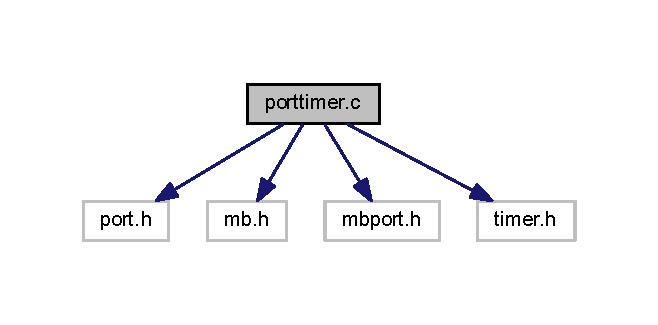
\includegraphics[width=316pt]{porttimer_8c__incl}
\end{center}
\end{figure}
\subsection*{Functions}
\begin{DoxyCompactItemize}
\item 
void \hyperlink{porttimer_8c_a4f589b4d10217312d963fc83b713d8ae}{Chip\+\_\+\+T\+I\+M\+E\+R\+\_\+\+Reset} (L\+P\+C\+\_\+\+T\+I\+M\+\_\+\+Type\+Def $\ast$p\+T\+MR)
\item 
B\+O\+OL \hyperlink{porttimer_8c_aded331146fcb93a6efe7c72100b06887}{x\+M\+B\+Port\+Timers\+Init} (U\+S\+H\+O\+RT us\+Tim1\+Timerout50us)
\item 
void \hyperlink{porttimer_8c_a541ea23eebb2aa5080f51b79e51c276c}{v\+M\+B\+Port\+Timers\+Enable} ()
\item 
void \hyperlink{porttimer_8c_ab2c2ac121ca4b26a14188f0c92efb827}{v\+M\+B\+Port\+Timers\+Disable} ()
\item 
void \hyperlink{porttimer_8c_a5f89e5f7418d3a10f49b2faeab3711dd}{T\+I\+M\+E\+R0\+\_\+\+I\+R\+Q\+Handler} (void)
\end{DoxyCompactItemize}


\subsection{Detailed Description}
Free\+Modbus Libary\+: B\+A\+RE Port Copyright (C) 2006 Christian Walter \href{mailto:wolti@sil.at}{\tt wolti@sil.\+at}

This library is free software; you can redistribute it and/or modify it under the terms of the G\+NU Lesser General Public License as published by the Free Software Foundation; either version 2.\+1 of the License, or (at your option) any later version.

This library is distributed in the hope that it will be useful, but W\+I\+T\+H\+O\+UT A\+NY W\+A\+R\+R\+A\+N\+TY; without even the implied warranty of M\+E\+R\+C\+H\+A\+N\+T\+A\+B\+I\+L\+I\+TY or F\+I\+T\+N\+E\+SS F\+OR A P\+A\+R\+T\+I\+C\+U\+L\+AR P\+U\+R\+P\+O\+SE. See the G\+NU Lesser General Public License for more details.

You should have received a copy of the G\+NU Lesser General Public License along with this library; if not, write to the Free Software Foundation, Inc., 51 Franklin St, Fifth Floor, Boston, MA 02110-\/1301 U\+SA

File\+: \begin{DoxyParagraph}{Id}
\hyperlink{porttimer_8c}{porttimer.\+c},v 1.\+1 2006/08/22 21\+:35\+:13 wolti Exp 
\end{DoxyParagraph}


\subsection{Function Documentation}
\index{porttimer.\+c@{porttimer.\+c}!Chip\+\_\+\+T\+I\+M\+E\+R\+\_\+\+Reset@{Chip\+\_\+\+T\+I\+M\+E\+R\+\_\+\+Reset}}
\index{Chip\+\_\+\+T\+I\+M\+E\+R\+\_\+\+Reset@{Chip\+\_\+\+T\+I\+M\+E\+R\+\_\+\+Reset}!porttimer.\+c@{porttimer.\+c}}
\subsubsection[{\texorpdfstring{Chip\+\_\+\+T\+I\+M\+E\+R\+\_\+\+Reset(\+L\+P\+C\+\_\+\+T\+I\+M\+\_\+\+Type\+Def $\ast$p\+T\+M\+R)}{Chip_TIMER_Reset(LPC_TIM_TypeDef *pTMR)}}]{\setlength{\rightskip}{0pt plus 5cm}void Chip\+\_\+\+T\+I\+M\+E\+R\+\_\+\+Reset (
\begin{DoxyParamCaption}
\item[{L\+P\+C\+\_\+\+T\+I\+M\+\_\+\+Type\+Def $\ast$}]{p\+T\+MR}
\end{DoxyParamCaption}
)}\hypertarget{porttimer_8c_a4f589b4d10217312d963fc83b713d8ae}{}\label{porttimer_8c_a4f589b4d10217312d963fc83b713d8ae}


 \subsubsection*{Chip\+\_\+\+T\+I\+M\+E\+R\+\_\+\+Reset }

Event Handler for G\+PI module \begin{DoxyVerb} @date                           DEC/02/2013
 @author                         FW_DEV_2
 @pre                            None
 @return                         None\end{DoxyVerb}
 

Definition at line 151 of file porttimer.\+c.



Here is the caller graph for this function\+:
\nopagebreak
\begin{figure}[H]
\begin{center}
\leavevmode
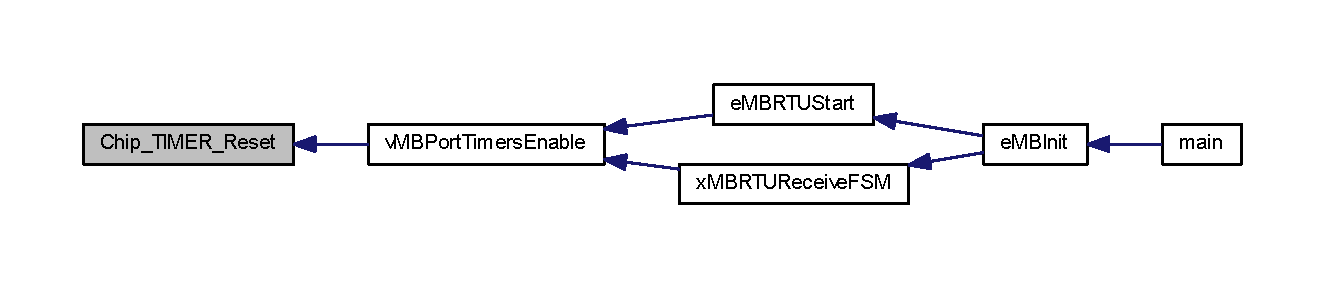
\includegraphics[width=350pt]{porttimer_8c_a4f589b4d10217312d963fc83b713d8ae_icgraph}
\end{center}
\end{figure}


\index{porttimer.\+c@{porttimer.\+c}!x\+M\+B\+Port\+Timers\+Init@{x\+M\+B\+Port\+Timers\+Init}}
\index{x\+M\+B\+Port\+Timers\+Init@{x\+M\+B\+Port\+Timers\+Init}!porttimer.\+c@{porttimer.\+c}}
\subsubsection[{\texorpdfstring{x\+M\+B\+Port\+Timers\+Init(\+U\+S\+H\+O\+R\+T us\+Tim1\+Timerout50us)}{xMBPortTimersInit(USHORT usTim1Timerout50us)}}]{\setlength{\rightskip}{0pt plus 5cm}B\+O\+OL x\+M\+B\+Port\+Timers\+Init (
\begin{DoxyParamCaption}
\item[{U\+S\+H\+O\+RT}]{us\+Tim1\+Timerout50us}
\end{DoxyParamCaption}
)}\hypertarget{porttimer_8c_aded331146fcb93a6efe7c72100b06887}{}\label{porttimer_8c_aded331146fcb93a6efe7c72100b06887}


 \subsubsection*{x\+M\+B\+Port\+Timers\+Init }

Event Handler for G\+PI module \begin{DoxyVerb} @date                           DEC/02/2013
 @author                         FW_DEV_2
 @pre                            None
 @return                         None\end{DoxyVerb}
 

Definition at line 229 of file porttimer.\+c.



Here is the caller graph for this function\+:
\nopagebreak
\begin{figure}[H]
\begin{center}
\leavevmode
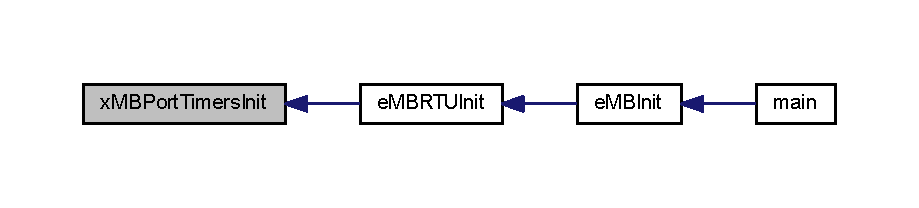
\includegraphics[width=350pt]{porttimer_8c_aded331146fcb93a6efe7c72100b06887_icgraph}
\end{center}
\end{figure}


\index{porttimer.\+c@{porttimer.\+c}!v\+M\+B\+Port\+Timers\+Enable@{v\+M\+B\+Port\+Timers\+Enable}}
\index{v\+M\+B\+Port\+Timers\+Enable@{v\+M\+B\+Port\+Timers\+Enable}!porttimer.\+c@{porttimer.\+c}}
\subsubsection[{\texorpdfstring{v\+M\+B\+Port\+Timers\+Enable()}{vMBPortTimersEnable()}}]{\setlength{\rightskip}{0pt plus 5cm}void v\+M\+B\+Port\+Timers\+Enable (
\begin{DoxyParamCaption}
{}
\end{DoxyParamCaption}
)}\hypertarget{porttimer_8c_a541ea23eebb2aa5080f51b79e51c276c}{}\label{porttimer_8c_a541ea23eebb2aa5080f51b79e51c276c}


 \subsubsection*{v\+M\+B\+Port\+Timers\+Enable }

Event Handler for G\+PI module \begin{DoxyVerb} @date                           DEC/02/2013
 @author                         FW_DEV_2
 @pre                            None
 @return                         None\end{DoxyVerb}
 

Definition at line 251 of file porttimer.\+c.



Here is the call graph for this function\+:
\nopagebreak
\begin{figure}[H]
\begin{center}
\leavevmode
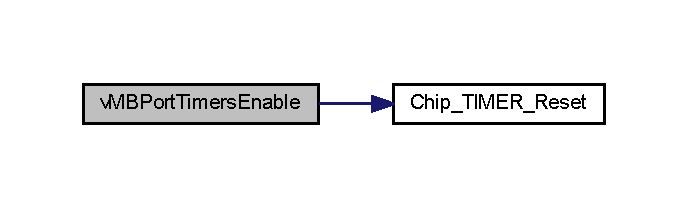
\includegraphics[width=330pt]{porttimer_8c_a541ea23eebb2aa5080f51b79e51c276c_cgraph}
\end{center}
\end{figure}




Here is the caller graph for this function\+:
\nopagebreak
\begin{figure}[H]
\begin{center}
\leavevmode
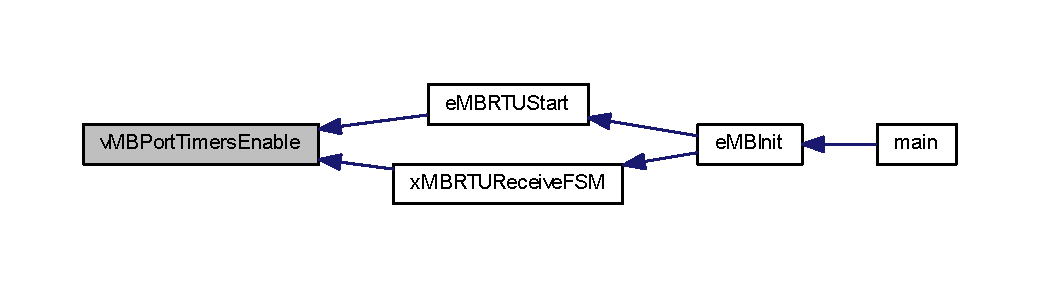
\includegraphics[width=350pt]{porttimer_8c_a541ea23eebb2aa5080f51b79e51c276c_icgraph}
\end{center}
\end{figure}


\index{porttimer.\+c@{porttimer.\+c}!v\+M\+B\+Port\+Timers\+Disable@{v\+M\+B\+Port\+Timers\+Disable}}
\index{v\+M\+B\+Port\+Timers\+Disable@{v\+M\+B\+Port\+Timers\+Disable}!porttimer.\+c@{porttimer.\+c}}
\subsubsection[{\texorpdfstring{v\+M\+B\+Port\+Timers\+Disable()}{vMBPortTimersDisable()}}]{\setlength{\rightskip}{0pt plus 5cm}void v\+M\+B\+Port\+Timers\+Disable (
\begin{DoxyParamCaption}
{}
\end{DoxyParamCaption}
)}\hypertarget{porttimer_8c_ab2c2ac121ca4b26a14188f0c92efb827}{}\label{porttimer_8c_ab2c2ac121ca4b26a14188f0c92efb827}


 \subsubsection*{v\+M\+B\+Port\+Timers\+Disable }

Event Handler for G\+PI module \begin{DoxyVerb} @date                           DEC/02/2013
 @author                         FW_DEV_2
 @pre                            None
 @return                         None\end{DoxyVerb}
 

Definition at line 276 of file porttimer.\+c.



Here is the caller graph for this function\+:
\nopagebreak
\begin{figure}[H]
\begin{center}
\leavevmode
\includegraphics[width=350pt]{porttimer_8c_ab2c2ac121ca4b26a14188f0c92efb827_icgraph}
\end{center}
\end{figure}


\index{porttimer.\+c@{porttimer.\+c}!T\+I\+M\+E\+R0\+\_\+\+I\+R\+Q\+Handler@{T\+I\+M\+E\+R0\+\_\+\+I\+R\+Q\+Handler}}
\index{T\+I\+M\+E\+R0\+\_\+\+I\+R\+Q\+Handler@{T\+I\+M\+E\+R0\+\_\+\+I\+R\+Q\+Handler}!porttimer.\+c@{porttimer.\+c}}
\subsubsection[{\texorpdfstring{T\+I\+M\+E\+R0\+\_\+\+I\+R\+Q\+Handler(void)}{TIMER0_IRQHandler(void)}}]{\setlength{\rightskip}{0pt plus 5cm}void T\+I\+M\+E\+R0\+\_\+\+I\+R\+Q\+Handler (
\begin{DoxyParamCaption}
\item[{void}]{}
\end{DoxyParamCaption}
)}\hypertarget{porttimer_8c_a5f89e5f7418d3a10f49b2faeab3711dd}{}\label{porttimer_8c_a5f89e5f7418d3a10f49b2faeab3711dd}


 \subsubsection*{T\+I\+M\+E\+R0\+\_\+\+I\+R\+Q\+Handler }

Event Handler for G\+PI module \begin{DoxyVerb} @date                           DEC/02/2013
 @author                         FW_DEV_2
 @pre                            None
 @return                         None\end{DoxyVerb}
 

Definition at line 319 of file porttimer.\+c.


%--- End generated contents ---

% Index
\backmatter
\newpage
\phantomsection
\clearemptydoublepage
\addcontentsline{toc}{chapter}{Index}
\printindex

\end{document}
